% arara: xelatex
% arara: xelatex
% arara: xelatex


% options:
% thesis=B bachelor's thesis
% thesis=M master's thesis
% czech thesis in Czech language
% english thesis in English language
% hidelinks remove colour boxes around hyperlinks

\documentclass[thesis=B,english]{css/FITthesis}[2019/12/23]

%\usepackage[utf8]{inputenc} % LaTeX source encoded as UTF-8
% \usepackage[latin2]{inputenc} % LaTeX source encoded as ISO-8859-2
% \usepackage[cp1250]{inputenc} % LaTeX source encoded as Windows-1250

% \usepackage{subfig} %subfigures
% \usepackage{amsmath} %advanced maths
% \usepackage{amssymb} %additional math symbols

\usepackage{dirtree} %directory tree visualisation
\usepackage{tikz} % Insert thesis task at the beginning
\usepackage{float} % Figures
\usepackage{amsthm} % Definitions, theorems ect.
\usepackage{amsmath}
\usepackage{amssymb}
\usepackage{mathtools} %rcases
\usepackage{graphicx}
\usepackage{subfig}
\usepackage{multirow} % cell merge
\usepackage{multicol}
\usepackage{tablefootnote}

\theoremstyle{definition}
\newtheorem{definition}{Definition}[section]

% % list of acronyms
% \usepackage[acronym,nonumberlist,toc,numberedsection=autolabel]{glossaries}
% \iflanguage{czech}{\renewcommand*{\acronymname}{Seznam pou{\v z}it{\' y}ch zkratek}}{}
% \makeglossaries

% % % % % % % % % % % % % % % % % % % % % % % % % % % % % % 
% EDIT THIS
% % % % % % % % % % % % % % % % % % % % % % % % % % % % % % 

\department{Department of Applied Mathematics}
\title{Statistical modeling of COVID-19 time series}
\authorGN{Oleh} %author's given name/names
\authorFN{Kuznetsov} %author's surname
\author{Kuznetsov Oleh} %author's name without academic degrees
\authorWithDegrees{Kuznetsov Oleh} %author's name with academic degrees
\supervisor{Ing. Dedecius Kamil, Ph.D.}
\acknowledgements{I express my sincere gratitude to my supervisor for this thesis Ing. Dedecius Kamil, Ph.D. It was thanks to him that I became interested in statistics and was motivated to study the topics covered in this work. The advice, guidance, and information received from him helped me deepen into this problem and achieve good results.

I am deeply grateful to my family (and especially my dear mother, father, and sister) for their support and opportunity to move to the Czech Republic and study at the Czech Technical University in Prague.

Last but not least, I would like to frankly acknowledge my friends for being with me during my studies.
}
\abstractCS{V letech 2020-2021 zažívá celý svět potíže způsobené globální epidemií nového viru SARS-CoV-2. Cílem této práce je statistická analýza časových řad souvisejících s pandemií COVID-19 v České republice a zkoumání využitelnosti modelů Facebook Prophet a Seasonal Autoregressive Integrated Moving Average (SARIMA) k analýze a predikci vývoje pandemických procesů. Tato práce propojuje globální změny, které nastaly ve vybraných časových řadách, s poskytnutými vládními omezeními (lockdown, nošení obličejové masky apod.).}
\abstractEN{In the years 2020-2021, the whole world is experiencing difficulties caused by the global epidemic of the new SARS-CoV-2 virus. This thesis aims at the statistical analysis of the time series related to the COVID-19 pandemic in the Czech Republic. It explores the usability of the Facebook Prophet and Seasonal Autoregressive Integrated Moving Average (SARIMA) models to analyze and predict the development of pandemic processes. Moreover, this thesis connects the global changes that occurred in the selected time series with the provided government restrictions (lockdown, wearing a face mask, and so on).}
\placeForDeclarationOfAuthenticity{Prague}
\keywordsCS{COVID-19, časové řady, prognózy časových řad, analýza časových řad, statistické modelování časových řad, Facebook Prophet, SARIMA  \clearpage}
\keywordsEN{COVID-19, Time series, Time series forecasting, Time series analysis, Statistical time series modeling, Facebook Prophet, SARIMA}
\declarationOfAuthenticityOption{1} %select as appropriate, according to the desired license (integer 1-6)
% \website{http://site.example/thesis} %optional thesis URL



\begin{document}

% \newacronym{CVUT}{{\v C}VUT}{{\v C}esk{\' e} vysok{\' e} u{\v c}en{\' i} technick{\' e} v Praze}
% \newacronym{FIT}{FIT}{Fakulta informa{\v c}n{\' i}ch technologi{\' i}}

\setsecnumdepth{part}
\chapter{Introduction}
At the beginning of 2020, the world was faced with a new disease called COVID-19. As already known, this infection is caused by the SARS-CoV-2 virus. In most cases, it occurs in the form of an acute respiratory infection. Moreover, it can cause various health complications and even death.

This virus was first detected in Wuhan, China. However, over time, it began to spread to other countries. As a result, we have witnessed a massive pandemic that has affected the entire world. Large numbers of sick people, overcrowded hospitals, and continuous government restrictive measures have become an integral part of the daily routine of countless people. Many lives depend on how the development of this outbreak will occur. Therefore, it is essential to understand this mechanism and be able to predict what will happen next \cite{Hu2021}. 

\section{Motivation}

Currently, the processes related to COVID-19 can be modeled using knowledge in statistics, programming, data mining, and data analysis. A good model can help you better understand the epidemic and even predict its development. The number of new cases, deaths, people cured, the number of active cases, the reproductive index, the number of free beds in hospitals --- all these are various objective metrics, data that can be used in modeling to describe the course of the pandemic.

Many experts are creating these models to improve the current situation in the world. However, in each country, the pandemic proceeds differently and the creation of models for a specific state also makes sense.

We was faced with the current world situation in the Czech Republic and everything that happened here has influenced our lives.

In light of the above, for this bachelor thesis we decided to study the modeling of processes related to the COVID-19 pandemic in this country.

\section{Objectives}

All the data that we can access can be described as a time series — a data set where all measurements are indexed with time. In 2021, there are a lot of different statistical models that can use this type of data to describe long-term processes. And for this thesis, we decided to select models named \textit{The Facebook Prophet} and \textit{Seasonal Autoregressive Integrated Moving Average} (SARIMA).

The Facebook Prophet is used to decompose the time series into specific components. It is also suitable for the detection of some points in time, after which the course of the pandemic was changed (changepoints). SARIMA was selected mainly for a comparison with the Facebook Prophet model. It uses a different principle based on the fact that the evolution of a time series depends on how it has developed in the past. You can find a more detailed description in the Chapter \hyperlink{ch3}{3}.

From the information-theoretic viewpoint, the COVID-19 pandemic is distinctive by an unprecedented amount of publically available data sets, mostly in the form of time series. 

The goal of this bachelor thesis is to study the properties of the selected time series and use the obtained information to fit the Facebook Prophet and SARIMA models to explain the evolution of the selected time series. After that, it is necessary to detect global trend changepoints and connect them with government decisions or other reasons. Moreover, this thesis aims to study the efficiency of using data slices starting from these changepoints in the modeling of epidemic processes. The final objective is to perform ex-post analyses of the results and evaluate predictions.

\section{Structure of the thesis}

This thesis consists of 3 chapters. Chapter \hyperlink{ch1}{1} aims to a more detailed disclosure of the theory related to time series, their properties and analysis. In Chapter \hyperlink{ch2}{2} you can find all necessary theory behind Facebook Prophet and SARIMA models. Chapter \hyperlink{ch3}{3} introduces practical application of selected models on COVID-19 related time series, results evaluation and discussion. 

\setsecnumdepth{all}
\chapter{Time Series. Properties and analysis}

\hypertarget{ch2}{This} chapter introduces the basic theory required for an understanding of time series, their properties, and the analysis approach. There also will be explained concepts like stochastic processes, mean value, variance, covariance, autocorrelation (ACF) and partial autocorrelation (PACF) functions, and time series decomposition. 

All the definitions without specific source mention are common for this field of statistics and can be found in many books (Cryer et al. \cite{cryer2008time}, Shumway et al. \cite{shumway2011}). 

\section{Time series and their basic analysis}
First of all, the formal definition of time series needs to be introduced. 
\begin{definition}[\textbf{Time series} \cite{Hyndman2018}]
\textit{Let $T$ be a set of time indices. The time series $Y$ is a sequence of numerical measurements taken at time steps $t \in T$. Formally: $Y = \left\{Y_{t}\;|\;t \in T\right\}$.
}
\end{definition}

In this thesis is considered that time is discrete, all time steps with neighboring indices are equidistant, so we can say, that $t \in Z$. 

\subsection{Goals of time series analysis}

To achieve the best possible results, it is necessary to establish the goals of the time series analysis. They can be formulated as:

\begin{itemize}
    \item \textbf{describing the monitored process} --- identifying the nature of the process represented by the selected time series.
    \item \textbf{forecasting} --- predicting the further development of the process using historical data.
\end{itemize}
\subsection{Real life time series illustrations}

Nowadays, sequentially collected data obtained from some measurements are widespread. There are a lot of different sources of this type of information: business, meteorology, agriculture, epidemiology, and many others.  In this subsection, we show some examples to give a basic idea of what such data looks like and what can be extracted from it.

All time series can be visualized as a graph. On the x-axis there are points in time, on the y-axis there are possible values of measurements taken at a given time.

For an example shown in Figure \ref{fig:daily_inf} we selected a data set that describes the number of people infected daily in the Czech Republic during the pandemic.

At first glance, we can say that this time series has seasonality and growing trend. However, there are different places where the growth rate changes, which may be caused by various cyclic processes, actions of the government, or other reasons.

\begin{figure}[t]
\centering
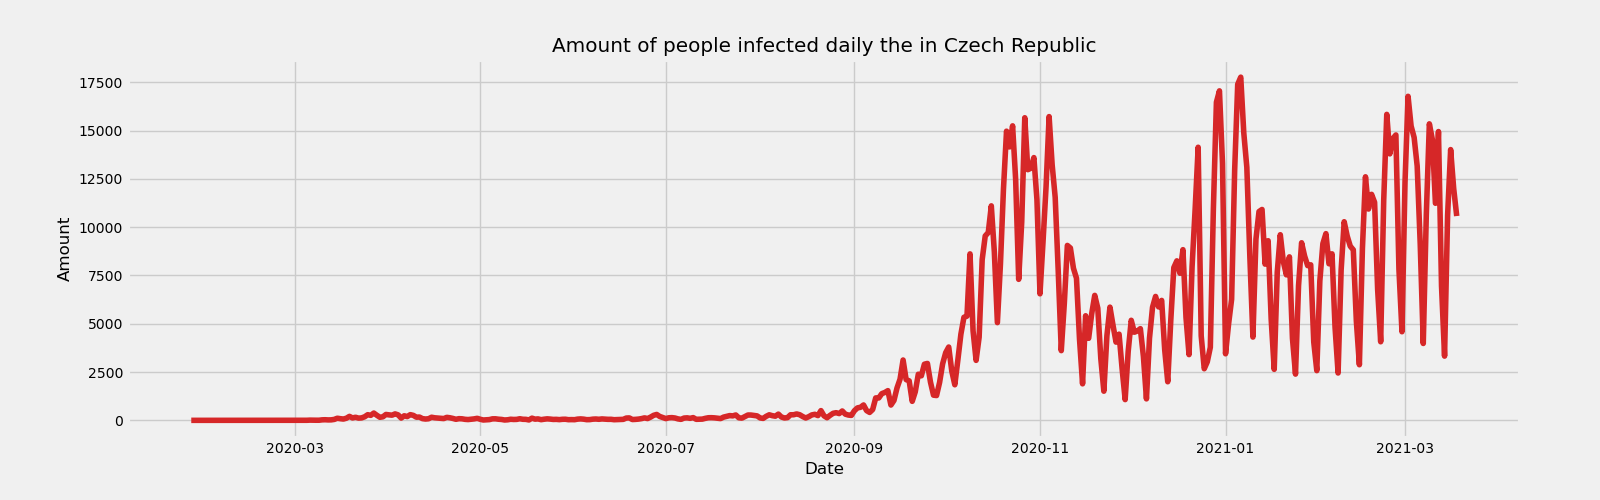
\includegraphics[width=1\textwidth, height=0.5\textwidth]{figures/chapter_02/daily_infected.png}
\caption{Amount of people infected daily in the Czech Republic.}
\label{fig:daily_inf}
\end{figure}

\subsection{Time series decomposition}

To describe the time series demonstrated in Figure \ref{fig:daily_inf_decomposed} it was necessary to use words like \textit{"trend"}, \textit{"seasonality"} and \textit{"cyclic"} \cite{Hyndman2018}. 

\begin{figure}[!ht]
\centering
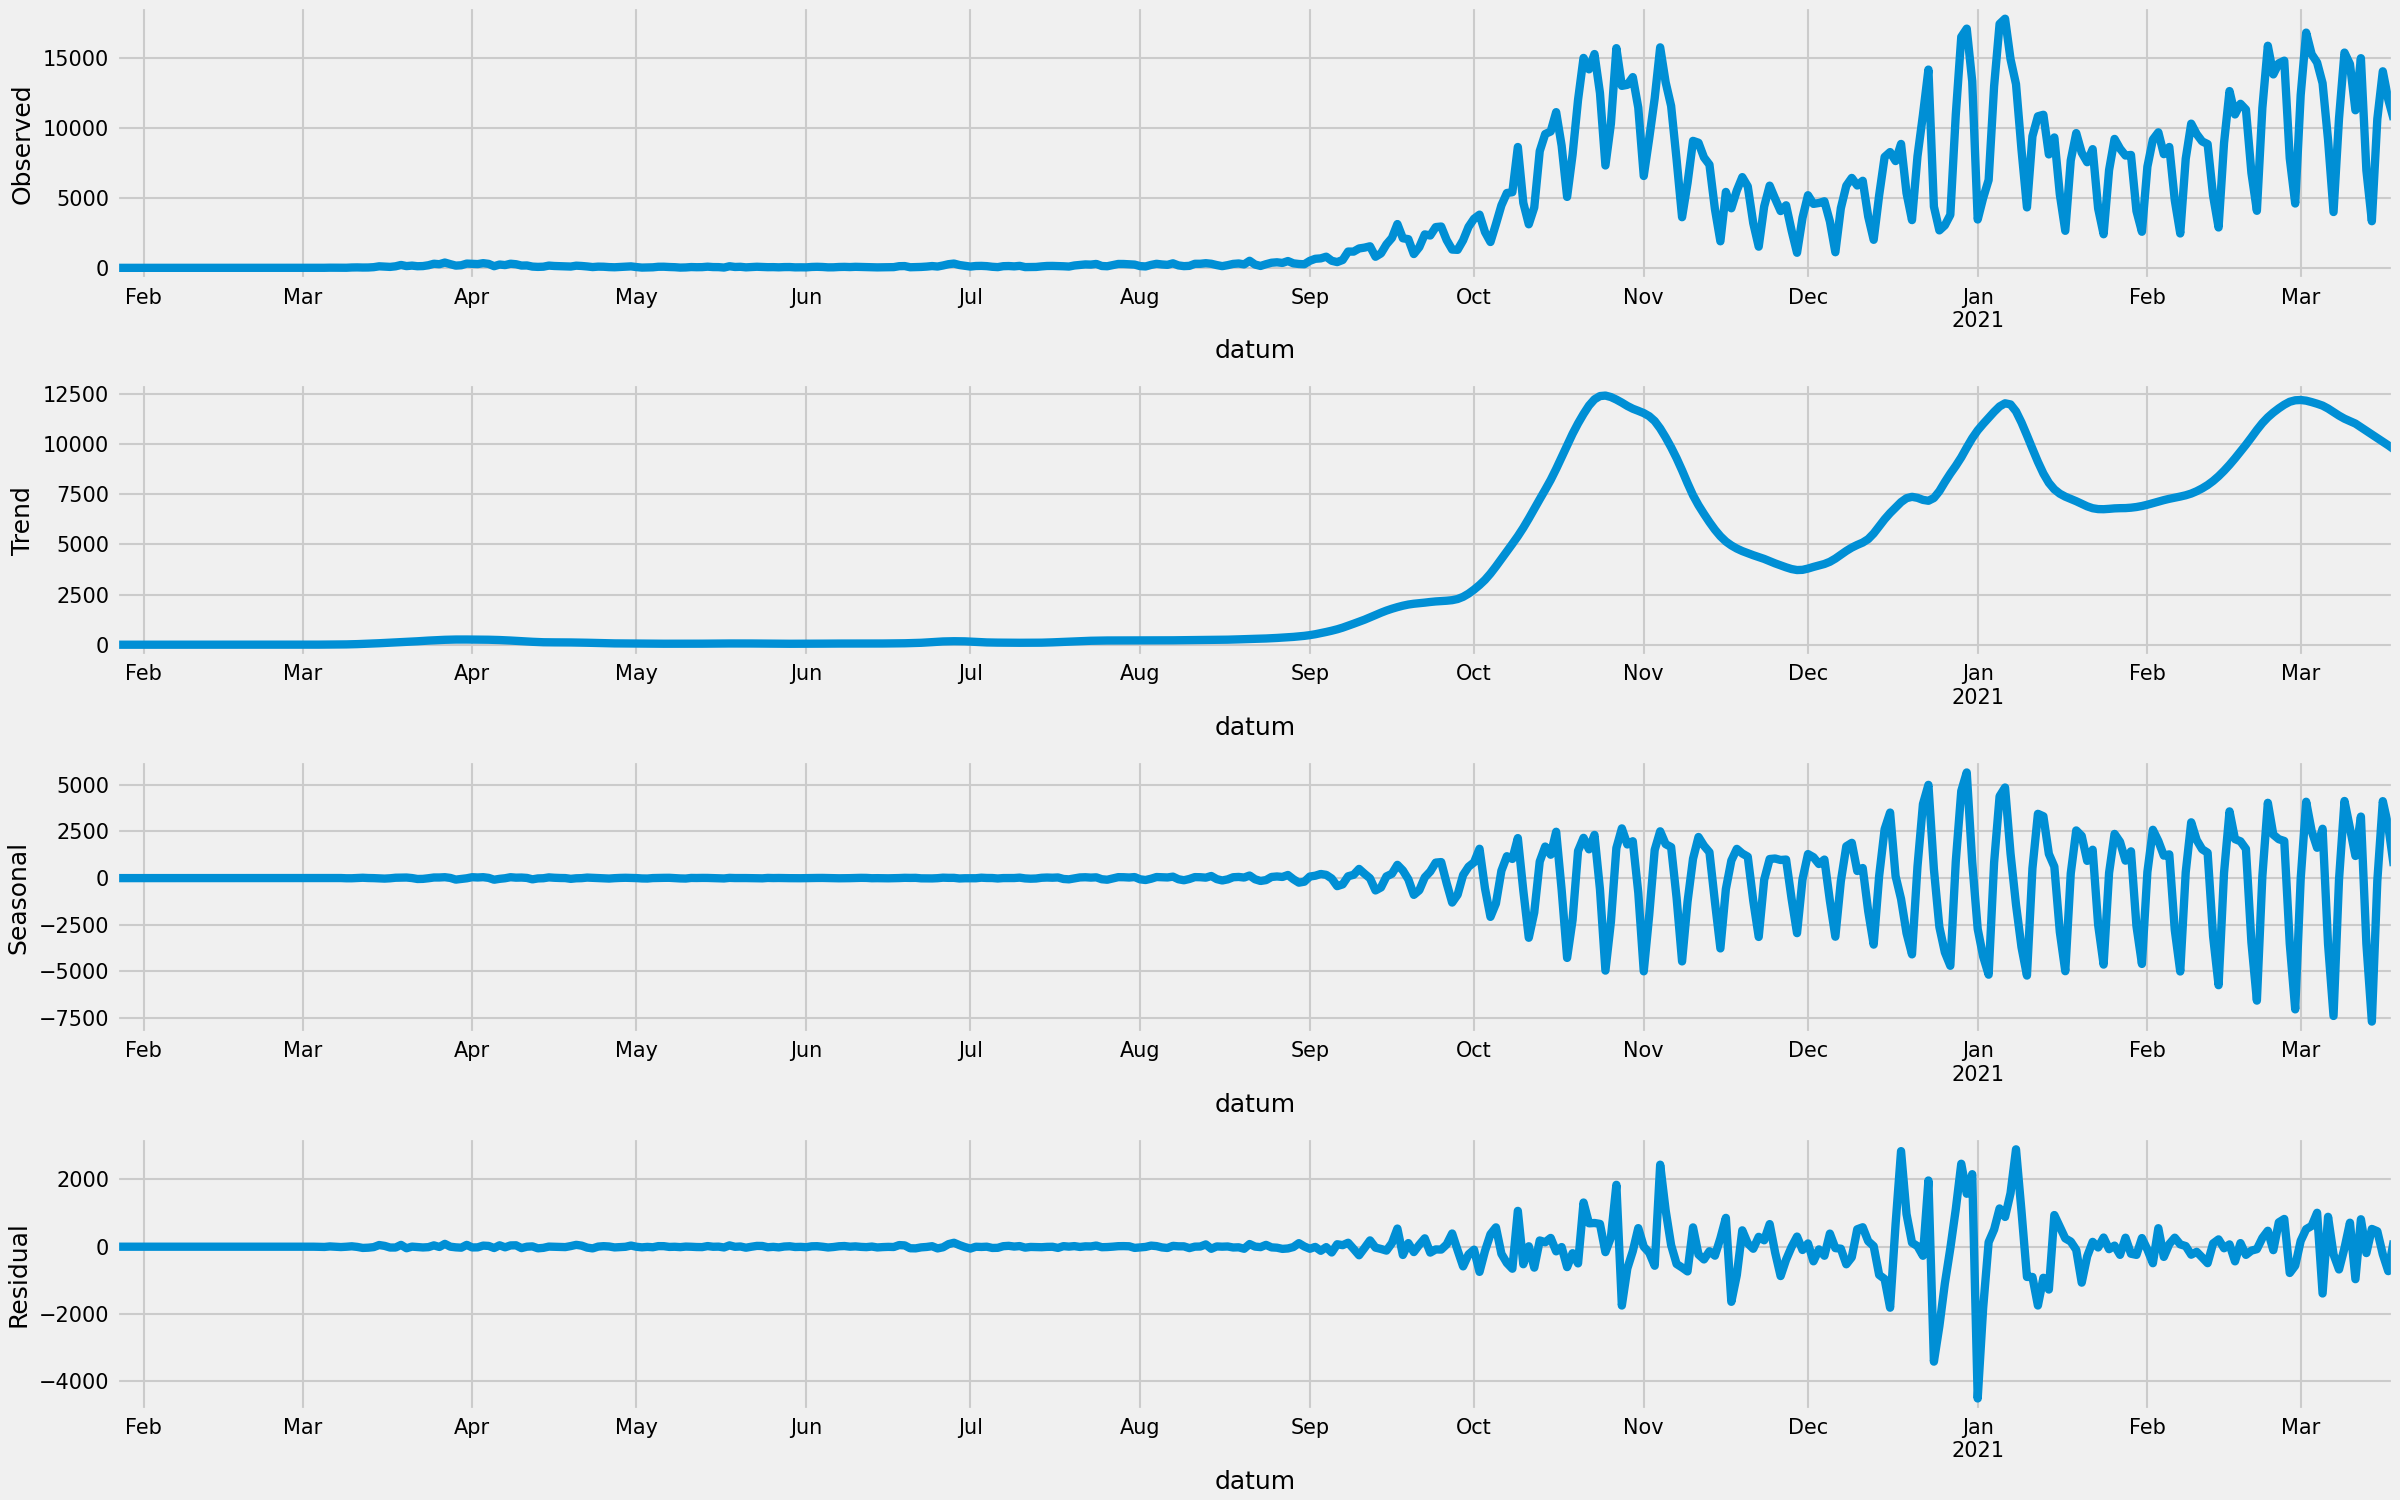
\includegraphics[width=1\textwidth, height=0.9\textwidth]{figures/chapter_02/daily_inf_decomposed.png}
\caption{Daily number of people infected: Decomposition into trend, seasonal, and residual components.}
\label{fig:daily_inf_decomposed}
\end{figure}

It is important to understand that almost all time series can be decomposed into specific parts, that is why we need to introduce a bunch of new definitions.

\begin{definition}[\textbf{Trend}]
\textit{The trend is the component of a time series that represents low frequency variations (long-term increase or decrease of mean value).}
\end{definition}

\begin{definition}[\textbf{Seasonal}]
\textit{The seasonal component represents periodically recurring, relatively regular and predictable (expected) development of the time series. For example, the temperature changes during the year.}
\label{def_seasonal}
\end{definition}

\begin{definition}[\textbf{Cyclic}]
\textit{The cyclic component of a time series represents changes that do not have a specific frequency.}
\end{definition}

Additionally, there are two main models created to describe the time series using these components (seasonal and cyclic components are denoted by one character):
\begin{itemize}
    \item \textbf{additive}:
    \begin{equation}
        Y_t = T_t + S_t + E_t,
    \label{eq_additive_model}
    \end{equation}
    \item \textbf{multiplicative}:
    \begin{equation}
        Y_t = T_t \cdot S_t \cdot E_t,
    \label{eq_multiplicative_model}
    \end{equation}
\end{itemize}
where $Y_t$ is a measured value at time step $t$, $T_t$ --- value of the trend component at the time step $t$, $S_t$ --- value of the seasonal and cyclic components at the time step $t$, $E_t$ --- part of the process at the time step $t$ that cannot be described by other components, also named \textit{residual}.

It is necessary to admit that we can transform the multiplicative model into additive using properties of the logarithm:
\begin{equation}
    \log (T_t \cdot S_t \cdot E_t) = \log T_t + \log S_t + \log E_t.
\end{equation}
Figure \ref{fig:daily_inf_decomposed} demonstrates a time series from the previous section and its decomposition into trend, seasonal, and residual components using the STL model \cite{cleveland1990stl}.

\section{Time series as a stochastic process}

To perform the analysis from the statistical point of view, it is important to understand that time series can be represented as a stochastic process. Therefore, we need to give its definition and describe the basic properties.

\begin{definition}[\textbf{Stochastic process} \cite{cryer2008time}]
\textit{Let $T$ be a set of time indices. Then stochastic process $Y$ is a set defined as $\left\{Y_{t}\;|\;t \in T\right\}$, where $Y_t$ is a random variable.}
\end{definition}
In this work, we will describe this processes in terms of mean value, variance, and covariance.

\subsection{Mean value, Variance, Covariance}

As previously stated, a stochastic process is a set of random variables. In other words, this process has a multivariate distribution and its properties depend on the distribution of each variable considered. Therefore, in this work we will specify terms that can describe this statistical distribution: mean value, variance, and covariance (first and second moments).

\begin{definition}[\textbf{Mean values, Variances, Covariances} \cite{cryer2008time}]
\textit{Let us assume the stochastic process $ Y = \left\{Y_{t}\;|\;t \in T\right\}$, where $T$ is a set of discrete time indices. Then:}
\begin{itemize}
    \item{\textit{\textbf{Mean value function} can be defined as} 
    \begin{equation}
    \mu_{t} = E(Y_{t}), \quad \forall t \in T,
    \label{eq_mean_value}
    \end{equation}}
    \item{\textit{\textbf{Variance} can be defined as 
    \begin{equation}
    \sigma^{2}_{t} = var Y_{t}, \quad \forall t \in T,
    \label{eq_variance}   
    \end{equation}}} 
    \item{\textit{\textbf{Autocovariance function} is specified as} \begin{equation}
    \gamma_{t_1, t_2} = cov(Y_{t_1}, Y_{t_2}), \quad \forall t_1, t_2 \in T,
    \label{eq_autocov_func}
    \end{equation} 
    \textit{where 
    \begin{equation}
    cov(Y_{t_1}, Y_{t_2}) = E[(Y_{t_1} - \mu_{t_1})(Y_{t_2} - \mu_{t_2})].
    \label{eq_covariance}
    \end{equation}}}
\end{itemize}
\end{definition}

\subsection{The Autocorrelation and Partial Autocorrelation functions}

Together with the basic time series moments, we need to introduce the terms of autocorrelation and partial autocorrelation functions. 

In essence, the autocorrelation of time series values denotes the linear (Pearson) correlation coefficient at different time steps. Now, it is important to introduce a more formal definition.

\begin{definition}[\textbf{Autocorrelation function} \cite{cryer2008time}]
\textit{Let us assume atime series $Y = \left\{Y_{t}\;|\; t \in T\right\}$ with mean value $\mu_{t}$ and variance $\sigma_{t}$ for each $t$. The autocorrelation coefficient for time steps $t_1$ and $t_{2}$ is given as}
\begin{equation}
\rho_{t_1, t_2} = corr(Y_{t_1}, Y_{t_2}) = \frac{E[(Y_{t_1} - \mu_{t_1})(Y_{t_2} - \mu_{t_2})]}{\sigma_{t_1}\sigma_{t_2}}, \quad \rho_{t_1, t_2} \in [-1, 1],
\label{eq_autocorrelation_func}
\end{equation}
\textit{on condition, that mean values and variances exist and are positive.}
\end{definition}

It is necessary to understand that its value for nonneighbouring time steps is effected by values of the time series in between. That is why we need to define the partial autocorrelation function, which represents the (auto) correlation of values at timestamps $t_1$ and $t_2$ after removing the effect of the intervening variables.

\begin{definition}[\textbf{Partial autocorrelation function} \cite{cryer2008time}]
\textit{Let us assume a time series $Y = \left\{Y_{t}\;|\; t \in T\right\}$. Then partial autocorrelation coefficient at lag $k$ will be defined as:}
\begin{equation}
\alpha_{t}(k) = corr(Y_{t}, Y_{t-k}\;|\; Y_{t-1}, Y_{t-2}, \ldots, Y_{t-k+1}), \quad \alpha_{t} \in [-1, 1].
\label{eq_partial_autocorrelation_func}
\end{equation}
\end{definition}
These functions can give us an understanding of the repetitive evolution of patterns in the time series. 

\subsection{Stationarity}

During the time series analysis, we might draw conclusions about its structure. Commonly, there are some reasonable simplifications and assumptions about this structure. In this thesis we will use the most important one called \textbf{stationarity}. The basic idea behind this term is that the statistical properties of the process, which generates the time series do not change over time. Specifically, we can highlight \textit{strict} and \textit{weak} stationary time series. 

\begin{definition}[\textbf{Strictly and weakly stationary time series} \cite{box1976time}]
\textit{Let us assume a time series $Y = \left\{Y_{t}\;|\; t \in T\right\}$, we say that this time series is:
\begin{itemize}
    \item \textbf{strictly} stationary if joint distribution of random variables $Y_{t_1}, \ldots, Y_{t_n}$ is equal to joint distribution of $Y_{t_1+\tau}, \ldots, Y_{t_n+\tau}$ for each $t_1, \ldots, t_n$ and $\tau$. 
    \item \textbf{weakly} stationary if it is invariant to time shifts within distribution moments of first and second order. That means:
    \begin{equation}
        E(Y_{t}) = \mu,
    \end{equation}
    and
    \begin{equation}
        cov(Y_{t}, Y_{t+\tau}) = \gamma(\tau),
    \end{equation}
    for each possible $t$ and $\tau$.
\end{itemize}}
\end{definition}

This thesis exploits the weekly stationarity term. Many statistical models used for time series modeling, such as ARMA (introduced in Chapter \hyperlink{ch2}{2}) assume (at least) a weekly stationary process. It is also possible to test the time series on stationarity using different statistical tests. According to Kwiatkowski et al. \cite{KWIATKOWSKI1992159}, it is possible using the combination of \textit{Dickey-Fuller} unit root test and \textit{Kwiatkowski–Phillips–Schmidt–Shin} (KPSS) stationarity test.

Dickey-Fuller test verifies the null hypothesis that the time series has unit roots against the alternative (no unit roots). However, sometimes it may be not enough to exclude, for example, trend-stationarity (stationary process with a trend). KPSS test evaluates the possibility that the time series is trend-stationary (null hypothesis) against the alternative that it is nonstationary. Different combinations of the results of these tests follow the different conclusions specified in Table \ref{tab:stat_tests}. 

\begin{table}[!hbt]
\centering
\resizebox{\textwidth}{!}{%
\begin{tabular}{|l|l|l|}
\hline
\textbf{DF test result} &
  \textbf{KPSS test result} &
  \textbf{Possible conclusion} \\ \hline
rejects null hypothesis &
  \begin{tabular}[c]{@{}l@{}}can not reject null \\ hypothesis\end{tabular} &
  stationarity \\ \hline
\begin{tabular}[c]{@{}l@{}}can not reject null \\ hypothesis\end{tabular} &
  rejects null hypothesis &
  nonstationarity \\ \hline
\begin{tabular}[c]{@{}l@{}}can not reject null \\ hypothesis\end{tabular} &
  \begin{tabular}[c]{@{}l@{}}can not reject null \\ hypothesis\end{tabular} &
  \begin{tabular}[c]{@{}l@{}}not enough data \\ (possible trend-stationarity)\end{tabular} \\ \hline
\begin{tabular}[c]{@{}l@{}}rejects null \\ hypothesis\end{tabular} &
  rejects null hypothesis &
  \begin{tabular}[c]{@{}l@{}}heteroscedasticity,\\ possible structural changes\end{tabular} \\ \hline
\end{tabular}%
}
\caption{Combination of the Dickey-Fuller and KPSS tests with possible conclusion.}
\label{tab:stat_tests}
\end{table}

\subsection{Examples of basic stochastic processes}

For the first example, we decided to select a process named white noise. 
\begin{definition}[\textbf{White noise}]
\textit{White noise is a stochastic process $\left\{ Y_{t}\right\}$, where:
\begin{equation}
E(Y_{t}) = 0,
\end{equation}
\begin{equation}
var(Y_{t}) = \sigma^{2} < \infty,
\end{equation}
\begin{equation}
cov(Y_{t}, Y_{t+\tau}) = \gamma(\tau) = 0.
\end{equation}}
\end{definition}

In other words, it is a process with a constant mean of zero, constant finite variance, and with independent and identically distributed (will be denoted as \textit{i.i.d.}) $Y_{t}$ and $Y_{t+\tau}$ for each possible $t$ and $\tau$. This leads to the conclusion, that this process is also \textit{strictly stationary}.

A special case of the white noise process is a normal (Gaussian) white noise, where $Y_{t} \sim \mathcal{N}(0,\,\sigma^{2})$. The Figure \ref{fig:white_noise} demonstrates an example of a time series generated using this type of process.

For the second example, we will introduce a random walk process. 

\begin{figure}[!htb]
  \centering
  \subfloat[a][Time series generated using the White noise process.]{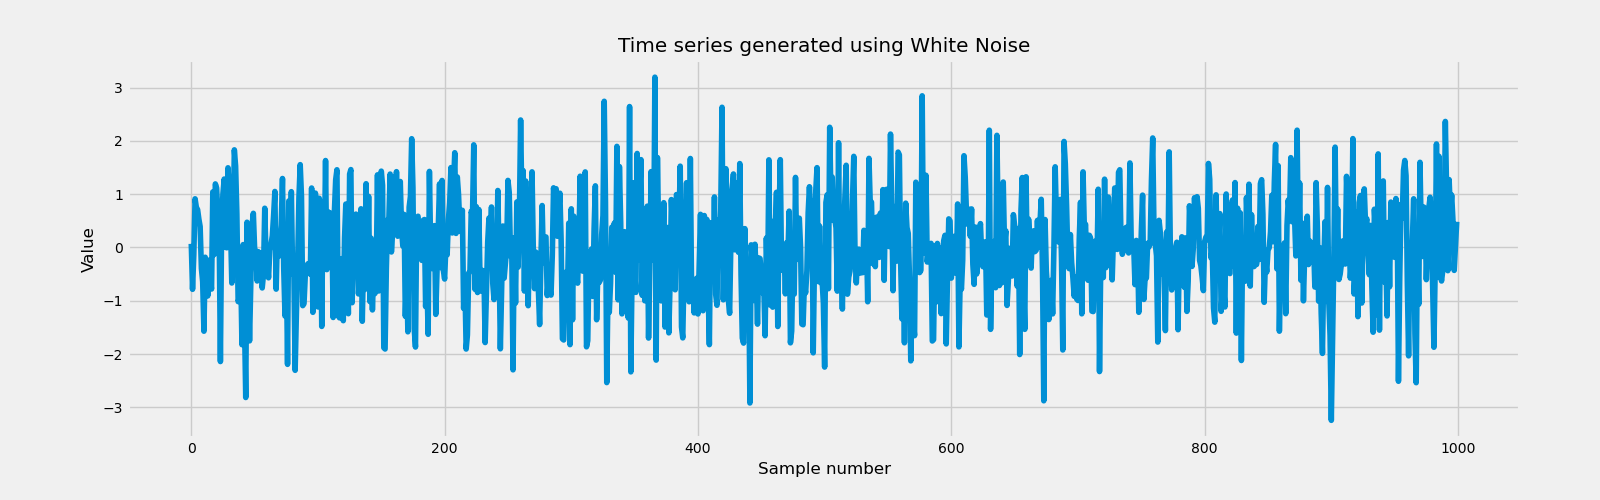
\includegraphics[width=1\textwidth, height=0.4\textwidth]{figures/chapter_02/white_noise.png} 
  \label{fig:white_noise}} \\
  \subfloat[b][Time series generated using the Random walk process.]{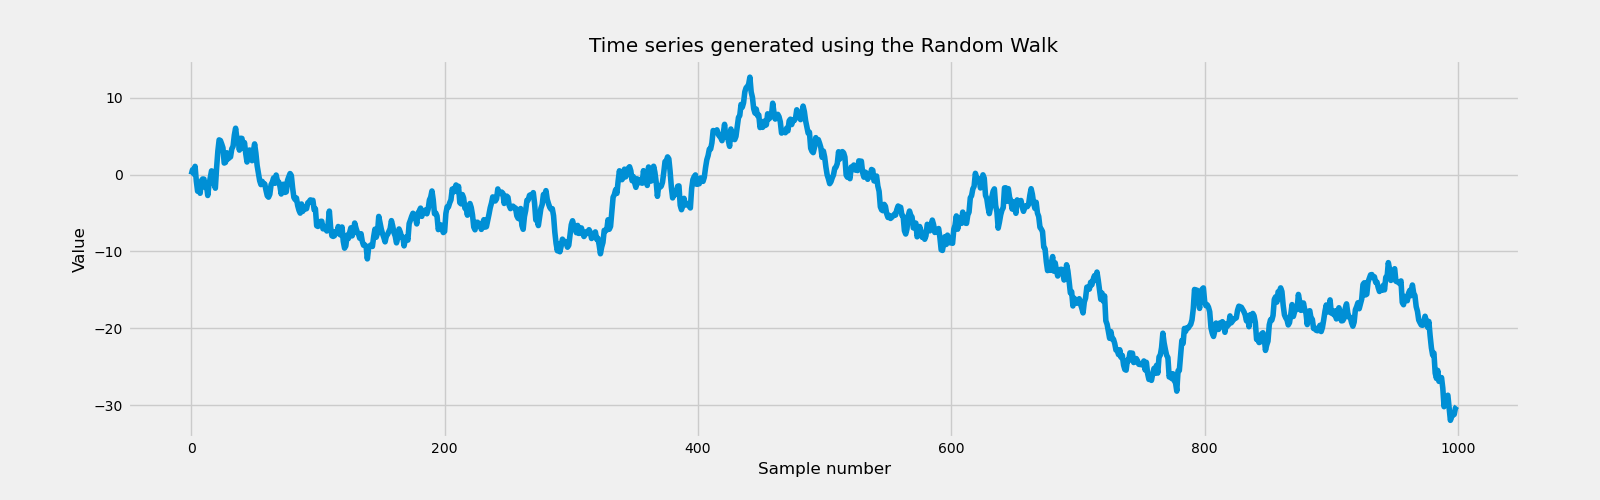
\includegraphics[width=1\textwidth, height=0.4\textwidth]{figures/chapter_02/random_walk.png} 
  \label{fig:random_walk}}
  \caption{Basic stochastic processes examples.} \label{fig:b_ex_ts}
\end{figure}

\begin{definition}[\textbf{Random walk}]
\textit{Let $e_{1}, e_{2}, \ldots$, be a sequence of independent, identically distributed random variables with zero mean value and variance $\sigma^2$ (White noise). Then the stochastic process $\left\{Y_{t}\;|\; t \in T\right\}$ will be a Random Walk if:
\begin{equation}
\begin{aligned}
Y_0 &= 0, \\ 
Y_t &= Y_{t-1} + e_{t},
\end{aligned}
\end{equation}
can also be written as 
\begin{equation}
Y_{t} = \sum_{i=1}^{t} e_i.
\end{equation}}
\label{def_random_walk}
\end{definition}
According to the attributes of the white noise and the properties of mean and variance, we can specify that $Y_t$ has zero mean and variance $t\sigma_{e}^{2}$. Furthermore, the covariance between $Y_{t_1} = \sum_{i=1}^{t_1} e_i$ and $Y_{t_2} = \sum_{i=1}^{t_2} e_i$, where $1 \leq t_1 < t_2$ is $t\sigma_{e}^{2}$. It follows from the covariance property (in the context of white noise):
\begin{equation}
cov(e_{i}, e_{j}) = 
\begin{cases}
    0, & \text{if } i \neq j,\\
    1, & \text{if } i = j.
\end{cases}
\label{eq_cov_white_noise}
\end{equation}
Based on the above, this process is nonstationary. In Figure \ref{fig:random_walk} there can be found an example of a time series generated using the random walk process.  


\section{Summary}
In this chapter, we have introduced the basic concepts behind the term "time series". We have formulated the definition of the time series, its decomposition and explored the representation of time series as a stochastic process. We have also described examples of basic processes that can generate time series.

\hypertarget{ch2}{\chapter{Theoretical description of selected statistical models}}

This chapter introduces a theoretical description of the two statistical models that were used in this thesis. They exploit fundamentally different principles based on which the process is modeled. We will describe the \textit{Facebook Prophet} model (interchangeably called \textit{the Prophet}), which is used for changepoints detection. Then the \textit{Seasonal Autoregressive Integrated Moving Average} (SARIMA) model will be covered. 

To argue our choice from the real-world applications point of view, it is necessary to introduce other studies that aim at the same problem. 

In Sengupta et al. \cite{Sengupta2020.06.25.20140004} different machine learning models such as various types of regression, LSTM (Long short-term memory) deep learning forecasting model, ARIMA, and the Facebook Prophet were compered during modeling of the COVID-19 time series related to India. Results reported by the authors of this study suggest that the ARIMA and Prophet models achieved more significant prediction results (on average) than most alternatives.

In Wang et al. \cite{WANG2020110058} authors used the Facebook Prophet logistic model for predicting the epidemic trend of COVID-19 in the whole world, Brazil, Russia, India, Peru, and Indonesia.

In Indhuja et al. \cite{indhuja2020prediction}, the Facebook Prophet model was used for modeling the explosive growth number of new cases in India.

In ArunKumar et al. \cite{ARUNKUMAR2021107161} were achieved quite good results in forecasting the dynamics of COVID-19 cases (confirmed, active, and death) for 16 countries around the world using the SARIMA model. 

In Ceylan et al. \cite{CEYLAN2020138817} the bunch of ARIMA models was used for forecasting the COVID-19 pandemic processes in Spain, Italy, and France. This study also refers to various researches made in the past that use (S)ARIMA models during the modeling of different diseases such as Malaria, Severe Acute Respiratory Syndrome, and so on.

Now we can move to the detailed description of the selected models.

\section{Facebook Prophet model}

The Facebook Prophet model was presented to the public and released in open source in 2017. The main objectives set forth by the creators are to simplify the modeling of processes whose evolution changes over time and to create a model that will be easily tuned during working on real-world projects.

This section mainly follows the explanation that can be found in the "Forecasting at Scale" article that introduces the Prophet model \cite{Taylor2018}.

\subsection{Main equation}

In essence, the Prophet uses a decomposable additive time series model with three basic components: trend, seasonal, and holidays. More formally:

\begin{definition}[\textbf{Prophet model main equation}]
\textit{Let us assume a time series $Y = \left\{Y_{t}\;|\;t \in T\right\}$ where  $Y_{t}$ is the value of observed variable $Y$ at timestamp $t$. The basic equation behind the Prophet model is
\begin{equation}
    Y_t = g(t) + s(t) + h(t) + e(t),
\label{eq_Prophet}
\end{equation}
where the variables are as follows:
\begin{itemize}
    \item $Y_{t}$ --- value of the observed variable in timestamp $t$.
    \item $g(t)$ --- trend component (non-periodic changes over time).
    \item $s(t)$ --- seasonal component (describes periodic changes over time).
    \item $h(t)$ --- holidays component (effect of irregular schedules $\geq$ 1 day long).
    \item $e(t)$ --- changes not covered by the model (error term).
\end{itemize}}
\end{definition}

Now, let us focus on each component separately.

\subsection{Trend component models} 
Prophet model has two options for trend modeling:
\begin{itemize}
    \item \textbf{Piecewise linear model}
    \item \textbf{Saturation growth model}
\end{itemize}

\subsubsection{Linear growth model}

We can use a linear model for processes where the maximum or minimum value of the observed variable is not defined, and we do not need saturation near it. However, it is well known that simple linear models cannot describe the process with lots of slope changes. 

For situations like this,  we must introduce a linear piecewise model. This model assumes the constant growth rate with changepoints. It is the standard model and used to be the default option in Prophet. 

To introduce the piecewise model equation, we need to formulate the definition of the vector of rate adjustments.
\begin{definition}[\textbf{Vector of rate adjustments}]
\textit{Let us assume that we have a time series with observed value $y$ which depends on time and has $C$ changepoints at timestamps $c_j$, $j$ = $1$, \ldots, $C$. That can be described as a vector of rate adjustments
\begin{equation}
    \boldsymbol{\delta} \in R^C,
\label{eq_adj_vector}
\end{equation}
where $\delta_{j}$ is a change in rate of trend growth at timestamp $c_j$.}
\end{definition}

According to this definition, the growth rate at any timestamp $t$ can be described as
\begin{equation}
    b + \sum_{j} \delta_{j}, \quad \text{while} \; t > c_j,
\end{equation}
\textit{where b $is$ a base growth rate at timestamp $t_{0}$.}
This rate change can be represented like a vector $a(t)$ in $\left\{0, 1\right\}^{C}$ such that: 
\begin{equation}
    a_{j}(t)=   \left\{
\begin{array}{ll}
      1, & \text{if} \; t \geq c_j, \\
      0, & \text{if} \;t < c_j. \\
\end{array} 
\right.  
\label{eq_used_changepoint_vector}
\end{equation}
The rate at timestamp $t$ then is 
\begin{equation}
b + \mathbf{a}(t)^{T}\boldsymbol{\delta}.
\label{eq_growth_rate_t}
\end{equation}

\begin{figure}[!ht]
\centering
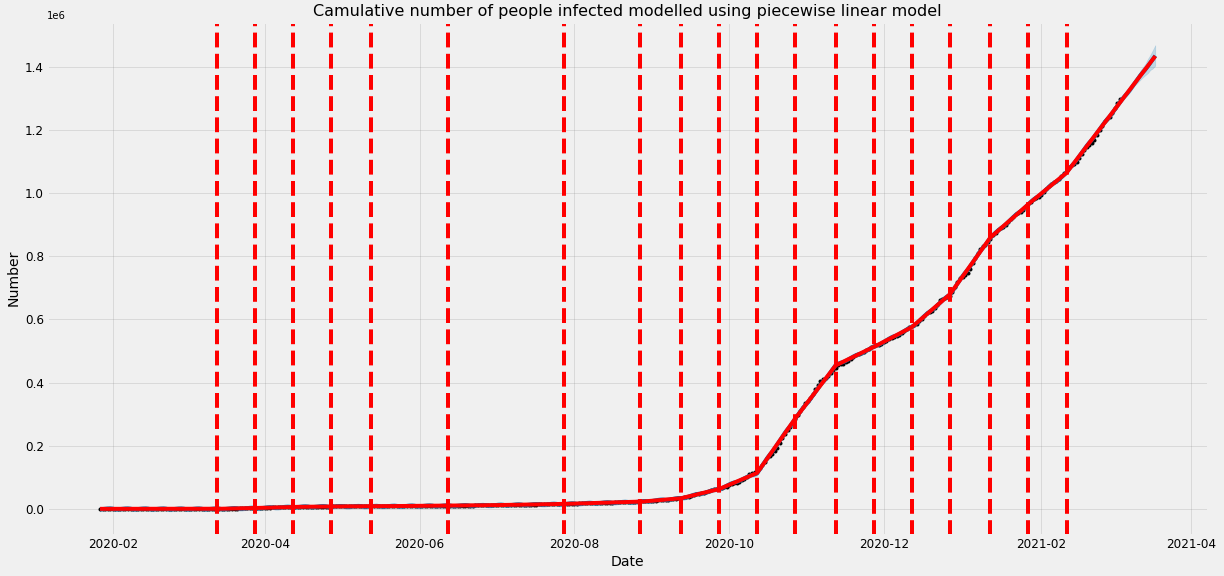
\includegraphics[width=1\textwidth, height=0.5\textwidth]{figures/chapter_03/picewise_model_example.png}
\caption{The cumulative number of people infected in Czech Republic time series modeled using the Facebook Prophet piecewise linear model with normally distributed changepoints for the first 90\% of the time series.}
\label{fig:piecewise_example}
\end{figure}

In addition to the base growth rate $b$, it is possible to tune the offset parameter $m$ (the value of the midpoint, where the slope changes its direction). This parameter is used to make the function continuous and connect the endpoints of the segments between changepoints:
\begin{equation}
    m + \mathbf{a}(t)^{T}\boldsymbol{\gamma},
\end{equation}
\textit{where components of the vector $\boldsymbol{\gamma}$ are defined as $\gamma_j = -c_{j}\delta_{j}$.}

After specifying all these parts, we can formulate the final equation of the piecewise linear model.

\begin{definition}[\textbf{Peicewice linear model}]
\textit{Let $g(t)$ be the value of trend component $g$ at timestamp $t$. Then the piecewise linear model equation can be defined as (we use extra parentheses for better visibility)}
\begin{equation}
   g(t) = (b + \mathbf{a}(t)^{T}\boldsymbol{\delta})t + (m + \mathbf{a}(t)^{T}\boldsymbol{\gamma}),
   \label{eq_piecewise_linear_model}
\end{equation}
\textit{where the variables of the equation are:
\begin{itemize}
    \item $b$ --- base trend growth rate.
    \item $\mathbf{a}(t)$ --- vector that specifies changepoints used for calculation of growth rate at timestamp $t$.
    \item $\boldsymbol{\delta}$ --- vector of rate adjustments.
    \item $m$ --- offset parameter.
    \item $\boldsymbol{\gamma}$ --- vector of offset adjustments.
\end{itemize}}
\end{definition}

According to this equation, we compute the value of the trend component $g$ at timestamp $t$ by multiplying the amount of time passed from the beginning of a process and the growth rate at this timestamp $t$. After this, we add an offset parameter $m$ corrected using the vector of offset adjustments $\boldsymbol{\gamma}$ to make this function continuous.
In this thesis, the piecewise linear model will be primary, because it correctly fits almost all selected COVID-19 time series.

Figure \ref{fig:piecewise_example} introduces the example of the Facebook Prophet piecewise linear model with normally distributed changepoints for the first 90\% of the time series. The vertical dashed lines pass through the timestamps where the changepoints are located. 

\subsubsection{Nonlinear Saturation growth model}
Sometimes, there is a time series forecasting task where it is necessary to deal with the maximum or minimum possible value. For example, at the beginning of an epidemic process, the government cannot deal with a fast increase in the number of people infected. In this case we can see explosive (non-linear), or even nearly exponential growth. In situations like this, we can use the logistic growth model, which can be written as 
\begin{equation}
    g(t) = \frac{C}{1 + e^{-k(t - m)}},
    \label{eq_saturating_model}
\end{equation}
\textit{where $C$ is the carrying capacity, $k$ is the growth rate, and $m$ --- an offset parameter.}
To deal with more complex situations, there are some improvements 

\begin{figure}[!ht]
\centering
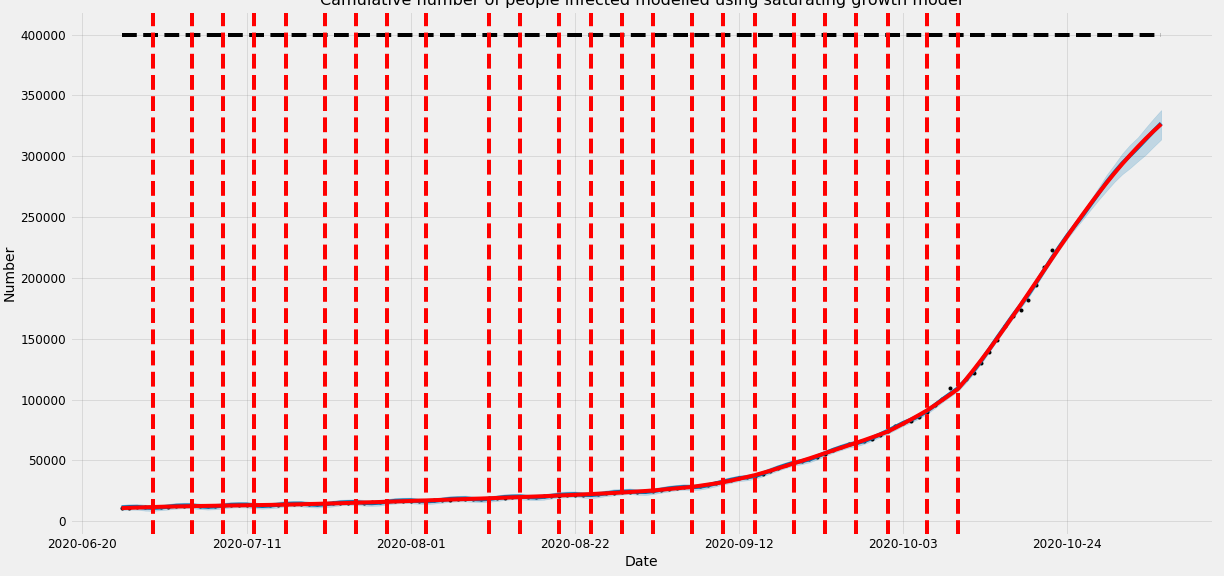
\includegraphics[width=1\textwidth, height=0.5\textwidth]{figures/chapter_03/logistic_model_example.png}
\caption{The cumulative number of people infected in Czech Republic time series (period of the explosive growth) modeled using the Facebook Prophet saturating growth model with normally distributed changepoints for the first 90\% of the time series.}
\label{fig:logistic_example}
\end{figure}

in the nonlinear version of the Prophet model. First, the constant carrying capacity $C$ was replaced with time-varying $C(t)$ (better for dynamic environments, where the maximum or minimum value changes over time). Second, the growth rate is changing (the same principle as in the linear model equation \ref{eq_growth_rate_t}). However, there is a difference associated with the offset parameter $m$. Its correct adjustment can be written as 
\begin{equation}
    \gamma_j = \bigg(c_j - m - \sum_{l < j} \gamma_l\bigg)\bigg(1 - \frac{b + \sum_{l < j} \delta_l}{b + \sum_{l \leq j} \delta_l}\bigg).
\end{equation}  
After all these corrections, we can formulate the final linear growth model equation.
\begin{definition}[\textbf{Logistic non-linear model}]
\textit{Let $g(t)$ be the value of trend component $g$ at timestamp $t$. Then the logistic (non-linear) model equation can be defined as
\begin{equation}
    g(t) = \frac{C(t)}{1 + exp(-(k + \mathbf{a}(t)^{T}\boldsymbol{\delta})(t - (m + \mathbf{a}(t)^{T}\boldsymbol{\gamma})))},
    \label{eq_logisic_model}
\end{equation}
where the variables are as follows 
\begin{itemize}
    \item $C(t)$ --- time-varying growth rate.
    \item $b$ --- base trend growth rate.
    \item $\mathbf{a}(t)$ --- vector that specifies changepoints used for calculation of growth rate at timestamp $t$.
    \item $\boldsymbol{\delta}$ --- vector of rate adjustments.
    \item $m$ --- offset parameter.
    \item $\boldsymbol{\gamma}$ --- vector of offset adjustments.
\end{itemize}}
\end{definition}

Figure \ref{fig:logistic_example} shows the part (with exponential growth) of the time series that describes cumulative number of people infected in the Czech Republic using the Facebook Prophet saturating growth model with normally distributed changepoints for the first 90\% of the time series. The capacity in the example is constant ($C(t) = 4000000$ for all $t$). 

\subsubsection{Automatic changepoints selection}
\label{sec:automatic_cp_detection}
The Prophet model supports manual changepoint selection. However, sometimes it is not available. In cases like this, for usage convenience, there is an automatic changepoint selection mechanism. It exploits a sparse prior on $\delta$ with equation \ref{eq_piecewise_linear_model} and \ref{eq_logisic_model}. In practice, we might specify a large number of changepoints (e.g., one or two per month) and use the prior $\delta_j \sim Laplace(0, \tau)$. 
\begin{definition}[\textbf{Classical Symmetric Laplace distribution }\cite{Kotz2001}]
\textit{We can say that a random variable has the Classical Laplace distribution on $(-\infty ; \infty)$ if its distribution is given by the density function 
\begin{equation}
    f(x, \theta, \tau) = \frac{1}{2\tau}exp\bigg(\frac{-|x - \theta|}{\tau}\bigg),
\end{equation} 
where $\theta \in (-\infty ; \infty)$ is the location parameter and $\tau > 0$ is the scale parameter.} 
\end{definition}
The parameter $\tau$ controls the flexibility of the rate change. It has no effect on the base growth rate, so if $\tau$ goes to 0, we receive standard linear or logistic growth.

According to the official Facebook Prophet documentation \cite{ProphetDoc}, it specifies 25 potential normally distributed changepoints for the first 80\% of the time series (by default). Subsequently, some of them are discarded by a procedure exploiting a sparse prior distribution. While fitting the trend component\footnote{\url{https://github.com/facebook/prophet/issues/933} --- explanation from a Facebook Prophet contributor on the official GitHub page}, the Prophet model minimalizes the sum of components of the vector of rate adjustments $\delta$. In other words, it tries to specify a set of changepoints $C$ with the biggest possible number of $\delta_j = 0$.

\subsubsection{Trend forecast uncertainty}

With just only historical data, the forecasted trend will have a constant growth rate. We need to extend the generative model forward to estimate the forecast uncertainty. In the Prophet model, we have $C$ changepoints over a history of $T$ time points, each of which has a rate change $\delta_j \sim Laplace(0, \tau)$. We can simulate future rate changes by replacing $\tau$ with the variance obtained from historical data. To perform this, we can use a maximum likelihood estimate of the rate scale parameter: \begin{equation}
    \lambda = \sum_{j=1}^{C} \delta_j.
\end{equation} We need to save historical changepoint frequency, so future changepoints  are randomly selected according to the following principle: \begin{equation}
    \forall j > T,   \left\{
\begin{array}{ll}
      \delta_j = 0, & \text{with probability } \frac{T- S}{T}, \\
      \delta_j \sim Laplace(0, \lambda), & \text{with probability } \frac{S}{T}. \\
\end{array} 
\right.
\end{equation} This means an assumption that in the future we will have the same frequency and magnitude of rate changes. After receiving lambda from historical data, we use a generative model to estimate possible trends and calculate uncertainty intervals. However, this assumption is quite strong, and these intervals may have not exact coverage. 

Moreover, as we already said, parameter $\tau$ controls rate change flexibility in historical data, so by increasing it, we can achieve lower training error but wider uncertainty intervals.

\subsection{Seasonal component}
A large number of time series can have multiperiod seasonality (yearly, weekly, daily, or quarterly). To handle these effects, the Prophet model contains the seasonality model, which is represented by periodic functions of $t$. One of the best possible options for modeling time series periodic patterns is to use the Fourier series. 

Thus, let $P$ be a constant expected time series period (for example, $P = 7$ for weekly data with the daily time scale). We can use a \textit{standard trigonometric polynomial of order $N$} (in fact, it is the Fourier series \cite{tolstov1976fourier})
\begin{equation}
    s(t) = \sum_{n=1}^{N}\bigg(a_{n}\cos\frac{2\pi nt}{P} + b_{n}\sin\frac{2\pi nt}{P}\bigg),
    \label{eq_fourier_seires}
\end{equation}
which can approximate a wide range of seasonal patterns. There is no intercept in this equation because we already have the trend component. 

According to Equation \ref{eq_fourier_seires}, the seasonal component fitting requires $2N$ parameters, that can be represented as a vector $\beta = [a_1, b_1, \ldots, a_N, b_N]^T$. The Prophet model does this by constructing a matrix of seasonal vectors for each timestamp t in historical and future data. For example, for weekly seasonality and $N = 5$: \begin{equation}
    \mathbf{X}(t) = \bigg[\cos\bigg(\frac{2\pi \cdot 1 \cdot t}{7}\bigg), \ldots, \sin\bigg(\frac{2\pi \cdot 5 \cdot t}{7}\bigg)\bigg].
\end{equation} After defining all this, we can formulate a definition of the seasonal component of the Prophet model.

\begin{definition}[\textbf{Facebook Prophet Seasonal component}]
\textit{Let us assume the Facebook Prophet model main equation $Y_t = g(t) + s(t) + h(t) + e(t)$, which represents the decomposed value of the observed variable $Y$  at a timestamp $t$, then the seasonal component $s(t)$ can be defined as
\begin{equation}
    s(t) = X(t)\boldsymbol{\beta},
\end{equation}
where 
\begin{itemize}
    \item $\mathbf{X}(t)$ is a matrix of seasonal vectors for each timestamp $t$.
    \item $\boldsymbol{\beta} \sim \mathcal{N}(0, \sigma^2)$ is a vector of fitting parameters that applies a smoothing prior to the seasonality.
\end{itemize}}
\end{definition}

In practice, there are several possible values of $N$, and there arises the need to discriminate among them (for example, a bigger value can lead to overfitting but allows modeling of seasonal patterns that change faster). The \textit{Akaike information criterion} (AIC)  or the \textit{Bayesian information criterion} (BIC) are two popular criteria that (loosely speaking) quantify the model quality \cite{doi:10.1177/0049124104268644}.

\subsection{Holidays component}

This component is used to handle important irregular schedules that can effect forecasts.

For each holiday $i$, let assume $D_i$ as a set of past and future dates of this holiday. Then, to indicate that a timestamp $t$ takes place during holiday and to assign each holiday a parameter $k_i$ which will indicate a corresponding change in the forecast we need to specify the matrix of regressors $\mathbf{Z}(t)$: \begin{equation}
    Z_{i}(t)=   \left\{
\begin{array}{ll}
      1, & \text{if } t \in D_i, \\
      0, & \text{if } t \notin D_i. \\
\end{array} 
\right.
\end{equation}
Now we can define the holidays component more formally.
\begin{definition}[\textbf{Facebook Prophet Holidays component}]
\textit{Let us assume the Facebook Prophet model main equation $Y_t = g(t) + s(t) + h(t) + e(t)$, which represents the decomposed value of the observed variable $Y$  at a timestamp $t$, then the holidays component $h(t)$ can be defined as
\begin{equation}
h(t) = \mathbf{Z}(t) \cdot \mathbf{k}.
\end{equation} where 
\begin{itemize}
    \item $\mathbf{Z}(t)$ is a matrix of regressors.
    \item $\mathbf{k}$ is a vector of corresponding (to selected holidays) changes in the forecast.
\end{itemize}}
\end{definition}

In addition to the curtain holiday date, we can define a few-day window around it to handle extra weekends, and so on. Moreover, the Prophet model uses $\mathbf{k} \sim \mathcal{N}(0, \sigma^2)$ to inflict a smoothing prior on the holidays component.

\subsection{Model fitting}

Fitting the Facebook Prophet model means the estimation of different model parameters described in the previous subsections (smoothing prior, Fourier Series order, etc.). It is an optimization task, where we need to minimize the error between historical data and model \cite{ProphetDoc}.

\subsection{Forecast accuracy evaluation}

The Prophet model uses a time series compatible version of the cross-validation concept. It specifies the cutoff points in historical data and for each of them fits the model. Then it forecasts the following points (the amount is specified by the forecast horizon) and compares the forecasted and actual values. To measure accuracy for each forecast made during cross-validation, the Prophet can use, for example, \textit{Mean Absolute Percentage Error} (MAPE) defined as 
\begin{equation}
    MAPE = \frac{100}{n} \sum_{t=1}^{n}\Big|\frac{Y_t - \hat{Y_t}}{Y_t}\Big|,
\end{equation}
where $n$ is an amount of forecasted points, $Y_t$ is the real value of the observed variable $Y$ at timestamp $t$, and $\hat{Y_t}$ is the forecasted value at timestamp $t$. This formulation is similar to the definition in Hyndman et al. \cite{Hyndman2018} (Chapter 3.4, Evaluating forecast accuracy).

After calculation of the error for each forecast made during the cross-validation, the Prophet model computes the mean between all these errors.

\subsection{Summary}

The Facebook Prophet is an additive model that can be used in complex real-world tasks. It supports trend growth rate changes, multivariate seasonality, and irregular schedules. It uses complex methods for parameter estimation and forecast accuracy evaluation. 

In addition to this, we found out that the Prophet model is widely used for modeling the COVID-19 pandemic processes. 

All of the above properties led us to the fact that the Prophet model would be a good choice for statistical modeling of time series related to the COVID-19 pandemic.

\section{SARIMA model}

In this section, we will introduce the basic concepts behind common parametric models, created and used in practice to describe real-world processes. This category was named \textit{Autoregressive Moving Average Models} (ARMA).

However, it is important to describe \textit{Autoregressive} and \textit{Moving Average} processes and models separately.

\subsection{Autoregressive process, AR model}

In essence, autoregressive processes are regressions on themselves \cite{cryer2008time}. The autoregressive process of $p$th-order means that value at timestamp $t$ depends on values at $p$ the most recent timestamps before it. For future work, we will need a formal definition for this type of a process.

\begin{definition}[\textbf{Autoregressive process of order $p$} \cite{shumway2011}]
\textit{Let us assume a stochastic process $Y = \left\{Y_{t}\;|\;t \in T\right\}$. This process can be named \textbf{the autoregressive of order $p$} if it has the following form
\begin{equation}
    Y_t = \phi_{1}Y_{t-1} + \phi_{2}Y_{t-2} + \ldots + \phi_{p}Y_{t-p} + e_t,
    \label{eq_ar_process}
\end{equation}
where the elements of the equation are 
\begin{itemize}
    \item $\phi_1, \ldots, \phi_p$ --- autoregressive coefficients ($\phi_p \neq 0$).
    \item $Y_{t-1}, \ldots, Y_{t-p}$ --- most recent $p$ past values.
    \item $e_t \sim \mathcal{N}(0, \sigma^2)$ --- Gaussian white noise at timestamp $t$, unless otherwise stated. In fact, it is part of the $Y_t$ that can not be described using $Y_{t-1}, \ldots, Y_{t-p}$.
\end{itemize}
If we talk about the AR process with nonzero mean value $\mu$, we need to replace $Y_t$ with $Y_t - \mu$ in Equation \ref{eq_ar_process},
\begin{equation}
    Y_t - \mu = \phi_{1}(Y_{t-1} - \mu) + \phi_{2}(Y_{t-2} - \mu) + \ldots + \phi_{p}(Y_{t-p} - \mu)+ e_t,
\end{equation}
or write
\begin{equation}
    Y_t = \phi_{0} + \phi_{1}Y_{t-1} + \phi_{2}Y_{t-2} + \ldots + \phi_{p}Y_{t-p} + e_t,
    \label{eq_ar_process_non_zero_mean}
\end{equation}
where $\phi_0 = \mu(1 -  \phi_0 -  \phi_1 - \ldots - \phi_p)$.}
\end{definition}

For modeling this process, we can use the autoregressive model (abbreviated as \textbf{AR}($p$), where $p$ is an order of the autoregressive process). However, this model assumes that the process is \textit{stationary}. 

\subsubsection{Stationarity of AR process}

First, we need to define the backshift operator \cite{shumway2011}, which allows a more compact and readable mathematical form of some definitions and equations that will occur in the following subsections. 

\begin{definition}[\textbf{Backshift operator}]
\textit{Let $Y_t$ be a value of an observed variable $Y$ at timestamp $t$. Then the \textbf{backshift operator} $B$ is defined by
\begin{equation*}
    BY_t = Y_{t-1},
\end{equation*}
and extended to powers $B^{2}Y_{t} = B(BY_t) = BY_{t-1} = Y_{t-2}$, and so on. Therefore, \begin{equation}
    B^{k}Y_t = Y_{t-k}.
    \label{eq_backshift_operator}
\end{equation}}
\end{definition} 

Now we can rewrite the AR model from Equation \ref{eq_ar_process} using the backshift operator as
\begin{equation}
\begin{aligned}
    Y_t &= \phi_{1}Y_{t-1} + \phi_{2}Y_{t-2} + \ldots + \phi_{p}Y_{t-p} + e_t, \\
    e_t &= Y_t - \phi_{1}Y_{t-1} - \phi_{2}Y_{t-2} - \ldots - \phi_{p}Y_{t-p} \\
        &= Y_t - \phi_{1}BY_t - \phi_{2}B^{2}Y_t - \ldots - \phi_{p}B^{p}Y_{t-p} \\
        &= (1 - \phi_{1}B - \phi_{2}B^2 - \ldots - \phi_{p}B^p)Y_t \\
        &= \phi(B)Y_t,
    \label{eq_ar_operator}
\end{aligned}
\end{equation}
where $\phi(B)$ is an \textbf{autoregressive operator}. In essence, it is the \textbf{AR characteristic polynomial}, that will be introduced later in Definition \ref{def_ar_char_polynomial}.

This form of Equation \ref{eq_ar_process} is widespread and used in equations related to more complex models.

Now, for understanding the stationarity of an AR process, we might also define its characteristic polynomial \cite{cryer2008time}.

\begin{definition}[\textbf{AR process characteristic polynomial}]
\textit{Let us assume an AR process with zero mean ($\phi_{0} = 0$), $Y_t = \phi_{1}Y_{t-1} + \phi_{1}Y_{t-1} + \ldots + \phi_{p}Y_{t-p} + e_t$, then the \textbf{AR polynomial} is defined as \begin{equation}
    \phi(x) = 1 - \phi_{1}x - \phi_{2}x^2 - \ldots - \phi_{p}x^{p},
    \label{eq_ar_polynomial}
\end{equation} where $\phi_1, \ldots, \phi_p$ are the regression coefficients, and $x^1, \ldots, x^p$ are the complex numbers.
Therefore, the corresponding \textbf{AR characteristic equation} is \begin{equation}
    1 - \phi_{1}x^{1} - \ldots - \phi_{p}x^{p} = 0.
    \label{eq_ar_pol_eq}
\end{equation}}
\label{def_ar_char_polynomial}
\end{definition}
According to the definition of the white noise process, we assume that $e_t$ is independent from $Y_t, Y_{t-1}, \ldots, Y_{t-p}$. Thus, according to the stationarity condition of AR process (Box et al. \cite{box1976time}), we can now formulate the following definition.

\begin{definition}[\textbf{Stationarity condition of AR($p$) process}]
Let us assume the AR process of order $p$ with the characteristic polynomial $\phi(x)$ and the corresponding characteristic equation $\phi(x) = 0$. This process is \textbf{stationary}
\begin{itemize}
    \item{if the roots of characteristic equation $\phi(x) = 0$ all exceeded $1$ in absolute value, or in other words}
    \item{if both following conditions are satisfied:
        \begin{equation}
            \begin{rcases*}
            \phi_1 + \phi_2 + \ldots + \phi_p < 1 \\
            |\phi_p| < 1 \\
            \end{rcases*}
        \label{eq_stationarity_cond}
        \end{equation}}
\end{itemize}
\label{def_ar_stationarity}
\end{definition} 
\subsubsection{AR process autocorrelation function}

Assuming a stationary AR process with zero mean, we can now define an important recursive relationship \cite{cryer2008time} for the autocorrelation function as \begin{equation}
\begin{aligned}
    \rho_0 &= 1, \\ 
    \rho_{-k} &= \rho_{k}, \\
    \rho_k &= \phi_{1}\rho_{k - 1} + \phi_{2}\rho_{k - 2} + \ldots + \phi_{p}\rho_{k - p}, & \text{ for } k \geq 1.
\end{aligned}
\end{equation} This relationship is used to compute the numerical values of $\rho_k$ for all possible $k$.

\begin{figure}[!ht]
\centering
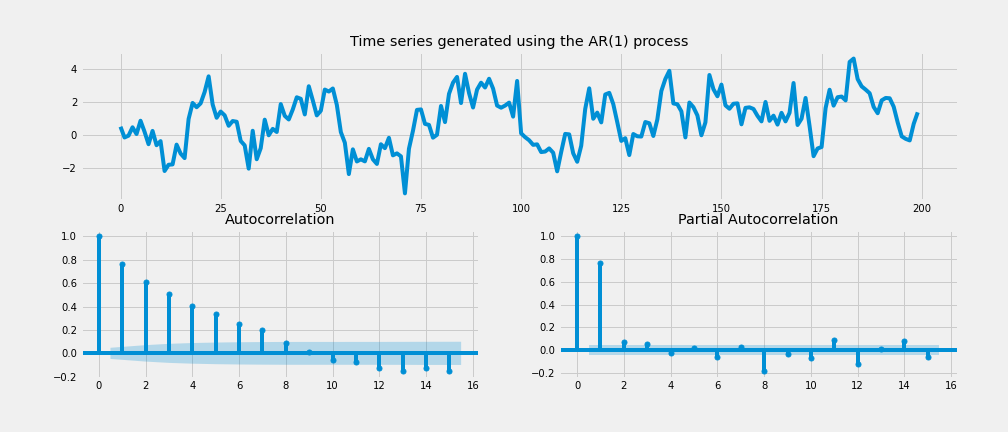
\includegraphics[width=1\textwidth, height=0.5\textwidth]{figures/chapter_03/ar_1.png}
\caption{The AR(1) process example and its ACF and PACF: $\phi_1 = 0.8, Y_0 = 0.5$.}
\label{fig:ar_1_example}
\end{figure}

\subsubsection{Example of the AR(1) process}

Figure \ref{fig:ar_1_example} shows the example of AR(1) process with $\phi_1 = 0.8, Y_0 = 0.5$. It also demonstrates the related autocorrelation and partial autocorrelation functions. 
According to the ACF, while increasing the lag, its value decreases, which indicates that the $Y_t$ in each timestamp $t$ is affected by the most recent previous value. 
The PACF shows that we have an expressive autocorrelation at lag 1 all other lags (which are cleared from the influence of earlier lags) have values that can be considered as non-contributory.

\subsection{Moving Average process, MA model}

As an alternative to an autoregressive model, where $Y_t$ is considered as a linear combination of previous $p$ observations, there are also exists a moving average model of order $q$ (denoted as MA($q$)) that assumes $Y_t$ as a linear combination of the white noise at timestamp $t$ and the white noise from $q$ previous most recent timestamps. 

\begin{definition}[\textbf{Moving average process of order $q$} \cite{shumway2011}]
\textit{Let us assume a stochastic process $Y = \left\{Y_{t}\;|\;t \in T\right\}$. This process can be named \textbf{the moving average of order $q$} if it has the following form
\begin{equation}
    Y_t = e_t + \theta_{1}e_{t-1} + \theta_{2}e_{t-2} + \ldots + \theta_{q}e_{t-q},
    \label{eq_ma_process}
\end{equation}
where the elements of the equation are 
\begin{itemize}
    \item $\theta_1, \ldots, \theta_q$ --- parameters\footnote{Sometimes, the MA($q$) model can be defined with negative coefficients:  $Y_t = e_t - \theta_{1}e_{t-1} - \theta_{2}e_{t-2} - \ldots - \theta_{q}e_{t-q}$.} ($\theta_q \neq 0$.).
    \item $e_{t}, \ldots, e_{t-q}$ --- the Gaussian white noise with zero mean and variance $\sigma_{e}^2$ at timestamp $t$ and $q$ more recent timestamps before $t$, unless otherwise stated.
\end{itemize}}
\end{definition}

The term Moving Average arises from the fact that we obtain $Y_t$ by applying the weights $1, \theta_1, \ldots, \theta_q$ to the variables $e_t, \ldots, e_{t-q}$ and then moving them and applying to $e_{t+1}, \ldots, e_{t-q+1}$ and so on \cite{cryer2008time}. 

For a more compact representation and integration into more complex equations, we can rewrite MA($q$) process in an equivalent form using the backshift operator (Equation \ref{eq_backshift_operator}) \begin{equation}
\begin{aligned}
    Y_t &= e_t + \theta_{1}e_{t-1} + \theta_{2}e_{t-2} + \ldots + \theta_{q}e_{t-q}\\
        &= e_t - + \theta_{1}Be_t + \theta_{2}B^{2}e_t + \ldots + \theta_{q}B^{q}e_t\\
        &= (1 - \theta_{1}B - \theta_{2}B^2 - \ldots - \theta_{q}B^q)e_t \\
        &= \theta(B)e_t,
    \label{eq_ma_operator}
\end{aligned}
\end{equation}
where $\theta(B)$ is the \textbf{moving average operator}. In fact, $\theta(B)$ is the \textbf{MA characteristic polynomial}, that will be introduced later in Definition \ref{def_ma_char_polynomial}.

Towards the end of the description of the general MA process, it is necessary to admit that:
\begin{itemize}
    \item{according to Equation \ref{eq_ma_process}, the MA($q$) process is \textbf{always stationary} for all values of $\theta_1, \ldots, \theta_q$,}
    \item{the autocorrelation function can be also computed using parameters $\theta_1, \ldots \theta_q$ as \begin{equation}
        \rho_k=   \left\{
    \begin{array}{ll}
      \frac{\theta_k + \theta_{1}\theta_{k+1} + \ldots + \theta_{q-k}\theta_{q}}{1 + \theta_{1}^{2} + \ldots + \theta_{q}^{2}}, & \text{for } k = 1, \ldots, q,\\
      0, & \text{for } k > q. \\
    \end{array} 
    \right.
    \end{equation}
    However, in contrast to the autocorrelation function of AR($p$) processes, it is limited to lag $q$ and can have a shape of almost anything for earlier lags \cite{cryer2008time}.}
\end{itemize}

\begin{figure}[!ht]
  \centering
  \subfloat[a][Time series generated using the MA(1) process with $\theta_1 = 0.5$.]{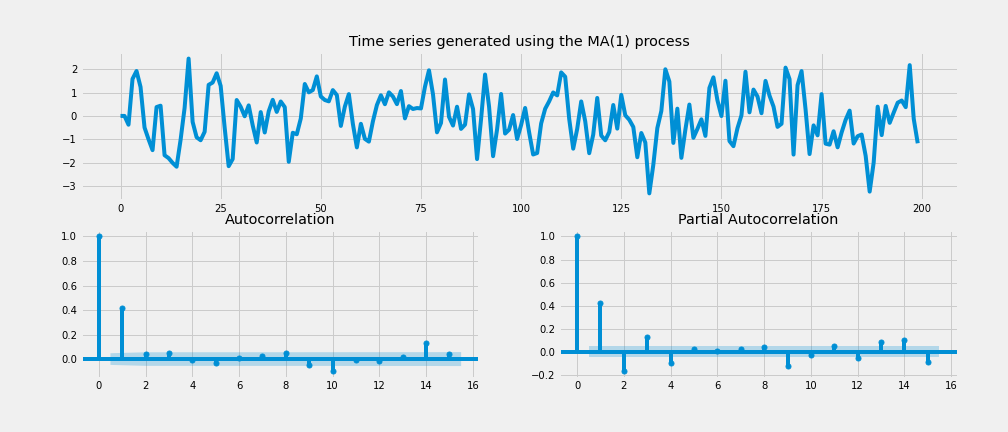
\includegraphics[width=1\textwidth, height=0.5\textwidth]{figures/chapter_03/ma_1_half.png}
  \label{fig:ma_1_half_example}} \\
  \subfloat[b][Time series generated using the MA(1) process with $\theta_1 = 2$.]{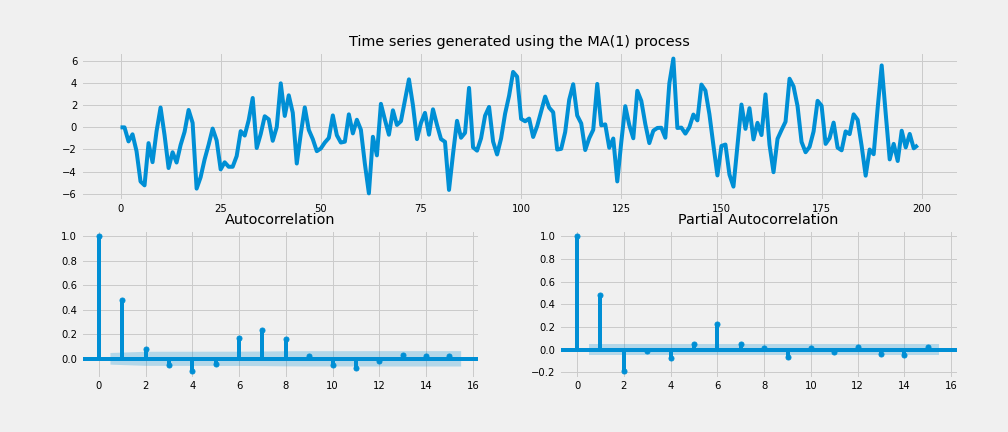
\includegraphics[width=1\textwidth, height=0.5\textwidth]{figures/chapter_03/ma_1_2.png} 
  \label{fig:ma_1_2_example}}
  \caption{Examples of the MA(1) process with identical value of ACF and PACF at lag 1.}
  \label{fig:ma_1_example}
\end{figure}

\subsubsection{Example of the MA(1) process}

Figure \ref{fig:ma_1_example} shows two examples of the MA(1) process with $\theta_1 = 0.5$ (Figure \ref{fig:ma_1_half_example}) and $\theta_1 = 2$ (Figure \ref{fig:ma_1_2_example}). It also demonstrates the related autocorrelation and partial autocorrelation functions. 

It is visible that the ACF and PACF drop after lag 1 ($q = 1$). Moreover, we are unable to guess the curtain value of $\theta_1$ parameter from the shape of these functions.

This find leads to the following property of the MA processes.

\subsubsection{Invertibility of the MA process}

According to Cryer et al. \cite{cryer2008time}, some MA($q$) processes can be reexpressed as an autoregression. Thus, if we consider MA(1) process (similar order as in previous section examples)
\begin{equation}
    Y_t = e_t + \theta_{1}e_{t-1},
\end{equation}
we can rewrite it as (with the similar form of $e_{t-1}$)
\begin{equation}
\begin{aligned}
e_t &= Y_t - \theta_{1}(Y_{t-1} - \theta_{1}e_{t-2})
&= Y_t - \theta_{1}Y_{t-1} + \theta_{1}^{2}e_{t-2}.
\end{aligned}
\end{equation}
If $|\theta_1| < 1$, we would not get exponential growth of $Y_t$ dependence on previous values and could continue infinitely
\begin{equation}
    e_t = Y_t - \theta_{1}Y_{t-1} - \theta_{1}^{2}Y_{t-2} - \ldots
\end{equation}
or 
\begin{equation}
    Y_t = e_t + \theta_{1}Y_{t-1} + \theta_{1}^{2}Y_{t-2} + \ldots
\end{equation}
It is now clear that the MA(1) model can be inverted into infinite-order autoregressive model if $|\theta_1| < 1$ and can be named \textbf{invertible}.

Before formulating the definition of the general MA($q$) model invertibility, we need to define its characteristic polynomial \cite{cryer2008time}.

\begin{definition}[\textbf{MA characteristic polynomial}]
\textit{Let us assume an MA process, $Y_t = \phi_{1}Y_{t-1} + \phi_{1}Y_{t-1} + \ldots + \phi_{p}Y_{t-p} + e_t$, then the \textbf{MA polynomial} is defined as \begin{equation}
    \theta(x) = 1 - \theta_{1}x - \theta_{2}x^2 - \ldots - \theta_{q}x^{q},
    \label{eq_ma_polynomial}
\end{equation} where $\theta_1, \ldots, \theta_p$ are the regression coefficients, and $x^1, \ldots, x^p$ are the complex numbers.
Therefore, the corresponding \textbf{MA characteristic equation} is \begin{equation}
    1 - \theta_{1}x^{1} - \ldots - \theta_{p}x^{p} = 0.
    \label{eq_ma_pol_eq}
\end{equation}}
\label{def_ma_char_polynomial}
\end{definition}

Now we can introduce the following definition.

\begin{definition}[\textbf{Invertibility of MA($q$) model} \cite{cryer2008time}]
\textit{Let us assume an MA process, $Y_t = \phi_{1}Y_{t-1} + \phi_{1}Y_{t-1} + \ldots + \phi_{p}Y_{t-p} + e_t$ and the model MA($q$) that describes this process. This model is \textbf{invertible}, if the are coefficients $\pi_j$ such that
\begin{equation}
    Y_t = \pi_{1}Y_{t-1} + \pi_{2}Y_{t-2} + \ldots + e_t,
\end{equation}
which is possible \textbf{if and only if} the roots of the corresponding characteristic equation $\theta(x) = 0$ \textbf{exceeded one in absolute value.}
\label{def_ma_invertibility}}
\end{definition}

Therefore, if we return back to the example in previous subsection, we may now notice that even if both processes have the same ACF, only one of them (with $\theta_1 = 0.5$) is invertible. 

To summarize this subsection, i would say that the \textbf{invertibility} of the MA process can be used to curtain estimation of its coefficients.

\subsection{Autoregressive Moving Average, ARMA model}

Sometimes, assuming that the process is only AR or only MA is not enough. In situations like this, we consider a mixed model named \textit{Autoregressive Moving Average} (denoted as ARMA($p, q$)) of orders $p$ and $q$. This leads to the following definition.

\begin{definition}[\textbf{Autoregressive Moving Average process of orders $p$ and $q$} \cite{shumway2011}]
\textit{Let us assume a stochastic process $Y = \left\{Y_{t}\;|\;t \in T\right\}$. This process can be named \textbf{the Autoregressive Moving Average of orders $p$ and $q$} if \begin{equation}
    Y_t = \phi_{1}Y_{t-1} + \ldots + \phi_{p}Y_{t-p} + e_t + \theta_{1}e_{t-1} + \ldots + \theta_{q}e_{t-q},
    \label{eq_arma_process}
\end{equation}
where the variables of the equation are 
\begin{itemize}
    \item $\phi_1, \ldots, \phi_p$ and $\theta_1, \ldots, \theta_q$ --- model parameters ($\phi_p \neq 0, \theta_q \neq 0$).
    \item $Y_{t-1}, \ldots, Y_{t-p}$ --- most recent $p$ past values.
    \item $e_{t}, \ldots, e_{t-q}$ --- the Gaussian white noise with zero mean and variance $\sigma_{e}^2$ at timestamp $t$ and $q$ more recent timestamps before $t$, unless otherwise stated.
\end{itemize}
If we talk about the ARMA process with nonzero mean value $\mu$, we need to replace $Y_t$ with $Y_t - \mu$ in Equation \ref{eq_arma_process}, \begin{equation}
\begin{aligned}
    Y_t - \mu &= \phi_{1}(Y_{t-1} - \mu) + \ldots + \phi_{p}(Y_{t-p} - \mu) + \\ &+ e_t + \theta_{1}e_{t-1} + \ldots + \theta_{q}e_{t-q},
\end{aligned}
\end{equation}
or write \begin{equation}
\begin{aligned}
    Y_t &= \phi_{0} + \phi_{1}Y_{t-1} + \ldots + \phi_{p}Y_{t-p} + e_t + \theta_{1}e_{t-1} + \ldots + \theta_{q}e_{t-q},
    \label{eq_arma_process_non_zero_mean}
\end{aligned}
\end{equation}
where $\phi_0 = \mu(1 -  \phi_0 -  \phi_1 - \ldots - \phi_p)$.}

\textit{The parameters $p$ and $q$ are usually called the autoregressive and the moving average orders, respectively. In addition, the process introduced in Equation \ref{eq_arma_process} can be described using the ARMA($p, q$) model if its AR part is \textbf{stationary} (Definition \ref{def_ar_stationarity}). Moreover, for the curtain estimation of the MA coefficients, we may use the MA process \textbf{invertiblity} (Definition \ref{def_ma_invertibility}).}
\label{def_arma_process}
\end{definition}

\begin{figure}[!ht]
\centering
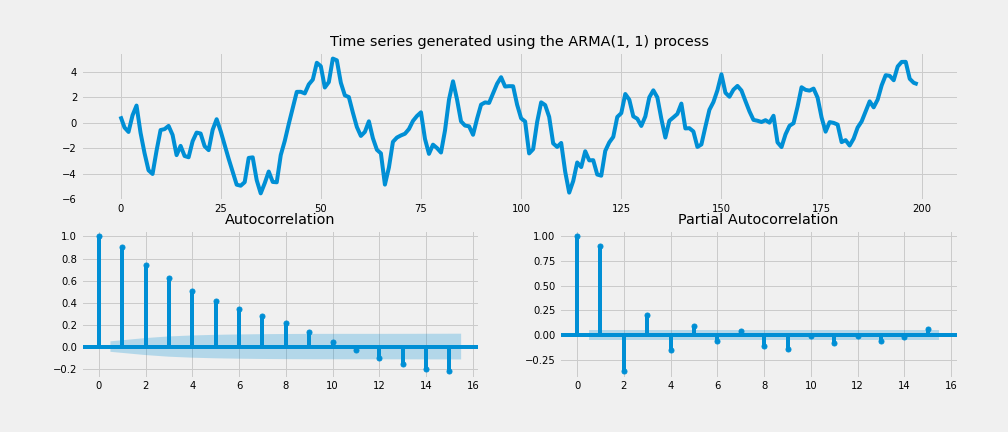
\includegraphics[width=1\textwidth, height=0.5\textwidth]{figures/chapter_03/arma_1_1.png}
\caption{The zero mean ARMA(1, 1) process example with its ACF and PACF: $\phi_1 = 0.8, \theta_0 = 0.5, Y_0 = 0.5$.}
\label{fig:arma_1_1_example}
\end{figure}

It is clear that if we assume $p = 0$, then the model will be a basic moving average of order $q$ or if we assume $q = 0$, then the model will be a basic autoregressive moving average of order $p$. 

Exploiting the fact that ARMA($p, q$) process is a mix of AR($p$) and MA($q$), we can rewrite Equation \ref{eq_arma_process} in a more compact form, using the autoregressive operator introduced in Equation \ref{eq_ar_operator} and the moving average operator introduced in Equation \ref{eq_ma_operator} as

\begin{equation}
    \phi(B)Y_t = \theta(B)e_t.
\end{equation}

\subsubsection{Example of ARMA(1, 1) process}

Figure \ref{fig:arma_1_1_example} demonstrates an example of
the time series generated with the ARMA(1, 1) process. The ACF and PACF indicate strong autocorrelation at lag 1. 

However, If we also take to account the example of the AR(1) process in Figure \ref{fig:ar_1_example}, we will notice that it is hard to guess the curtain order of the mixed ARMA model. The shapes of its ACF and PACF are similar to those related to the standard AR(1) process.  

\subsection{Integrated time series: Differencing \& ARIMA model}

All models introduced in the previous subsections required a (weakly) stationary process. However, a large number of real-life problems consist of nonstationary time series generated by nonstationary processes. For example, the random walk process (introduced in Definition \ref{def_random_walk}) has a constant mean but has no deterministic trend. It means that it can not be described using a model that assumes, for example, a stationary time series with an added time-varying mean $\mu$.

It is clear from the definition of random walk that it is a nonstationary AR(1) process given by
\begin{equation}
    Y_t = Y_{t-1} + e_t.
\end{equation}
However, by rewriting this process using the \textbf{first difference} defined as
\begin{equation}
    \nabla Y_t = Y_t - Y_{t-1},
\end{equation}
we will receive the following equation
\begin{equation}
    \nabla Y_t = e_t,
\end{equation}
which describes a stationary process. It is clear that this example can be easily extended to get not just the white noise.

In Cryer et al. \cite{cryer2008time} we can find an example, which assumes the process defined as \begin{equation}
    Y_t = M_t + X_t,
\label{eq_example_diff_ts}
\end{equation}
where $M_t$ is an almost constant (either deterministic or stochastic) series. It is possible to approximate the value of $M$ at timestamp $t$: \begin{equation}
    \hat{M_t} = \frac{1}{2}(Y_t + Y_{t-1}).
\end{equation} After this, we can get rid of $M_t$ in Equation \ref{eq_example_diff_ts} and receive \begin{equation}
    Y_t - \hat{M} = Y_t - \frac{1}{2}(Y_t - Y_{t-1}) = \frac{1}{2}(Y_t - Y_{t-1}) = \frac{1}{2}\nabla Y_t,
\end{equation}
which is a \textbf{constant multiple of the first difference at lag 1}.

This example assumes that $M$ in Equation \ref{eq_example_diff_ts} is stochastic and its changes are driven by the random walk process (along with $Y_t$), such that \begin{equation}
\begin{aligned}
    Y_t &= M_t + e_t, \\
    M_t &= M_{t-1} + \varepsilon_t,
\end{aligned}
\end{equation}
where $e_t$ and $\varepsilon_t$ are independent values generated by the white noise process. Then \begin{equation}
    \nabla Y_t = \nabla M_t + \nabla e_t = \varepsilon_t + e_t - e_{t-1},
\label{eq_example_diff_then_ma}
\end{equation}
which will have the autocorrelation function of an MA(1) process. According to Cryer et al. \cite{cryer2008time}, we can study $\nabla Y_t$ from Equation \ref{eq_example_diff_then_ma} as stationary.

It is also possible to formulate assumptions which will lead to a time series that will be stationary after the second difference, and so on. This motivates the following definition.

\begin{definition}[\textbf{Integrated Moving Average process ARIMA($p, d, q$)} \cite{cryer2008time}]
\textit{
Let us assume a stochastic process $Y = \left\{Y_{t}\;|\;t \in T\right\}$. This process can be described using \textbf{the Integrated Moving Average model} if the $d$th difference 
\begin{equation}
    W_t = \nabla^d Y_t
\end{equation}
is a \textbf{stationary ARMA process} introduced in Definition \ref{def_arma_process}. If $W_t$ can be described using ARMA model, we can say that $Y_t$ is an \textbf{ARIMA($p, d, q$) process}.
}
\end{definition} 
The most common values of $d$ that can occur in practice are 1 or 2. Therefore, we can introduce ARIMA process equation with $W_t = Y_t - Y_{t-1}$: \begin{equation}\begin{aligned}
W_t &= \phi_{1}W_{t-1} + \phi_{2}W_{t-2} + \ldots + \phi_{p}W_{t-p} \\ 
    &+ e_t + \theta_{1}e_{t-1} + \theta_{2}e_{t-2} + \ldots + \theta_{q}e_{t-q}.
\end{aligned}
\label{eq_arima_process}
\end{equation}
It is possible to rewrite this equation in terms of the original model, \begin{equation}
\begin{aligned}
Y_t - Y_{t-1} &= \phi_{1}(Y_{t-1} - Y{t-2}) + \phi_{2}(Y_{t-2} - Y{t-3}) \\
&+ \ldots + \phi_{p}(Y_{t-p} - Y_{t-p-1})\\
&+ e_t + \theta_{1}e_{t-1} +  e_t + \theta_{1}e_{t-1} + \ldots + \theta_{q}e_{t-q},
\end{aligned}
\end{equation}
or using \textbf{the difference equation form} of the model \cite{cryer2008time} as \begin{equation}
\begin{aligned}
Y_t &= (1 + \phi_{1})Y_{t-1} + (\phi_{2} - \phi_{1})Y_{t-2} + (\phi_{3} - \phi_{2})Y_{t-3}\\
&+ \ldots + (\phi_{p} - \phi_{p-1})Y_{t-p} - \phi_{p}Y_{t-p-1} \\
&+ e_t + \theta_{1}e_{t-1} +  e_t + \theta_{1}e_{t-1} + \ldots + \theta_{q}e_{t-q}.
\end{aligned}
\label{eq_diff_eq_form}
\end{equation}
In accordance with Equation \ref{eq_diff_eq_form} we now have ARMA($p+1, q$) process. However, the corresponding AR characteristic polynomial is \begin{equation}
\begin{aligned}
    1 &- (1 + \phi_{1})x - (\phi_{2} - \phi_{1})x^2 - (\phi_{3} - \phi_{2})Y_{t-3})x^3 \\
    &- \ldots - (\phi_{p} - \phi_{p-1})x^p `+ \phi_{p}x^{p+1}\\
    &= (1 - \phi_{1}x - \phi_{2}x^2 - \ldots - \phi_{p}x^p)(1 - x),
\end{aligned}
\end{equation}
which shows the root $x = 1$ that applies \textit{nonstationarity}. However, we obtain the remaining roots from the characteristic polynomial of the \textit{stationary process $\nabla Y_t$}. 

\begin{figure}[!ht]
\centering
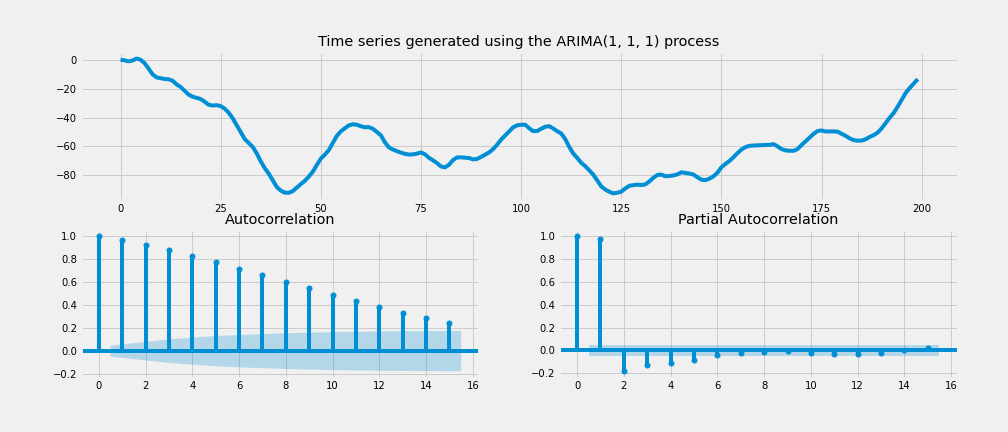
\includegraphics[width=1\textwidth, height=0.5\textwidth]{figures/chapter_03/arima_1_1_1.png}
\caption{The ARIMA(1, 1, 1) process example with its ACF and PACF: $\phi_1 = 0.8, \theta_0 = 0.5, Y_0 = 0.5$.}
\label{fig:arima_1_1_1_example}
\end{figure}

We can also formulate the ARIMA($p, d, q$) model more a more compact way using the autoregressive and moving average operators as \begin{equation}
    \phi(B)\nabla^{d}Y_t = \theta(B)e_t.
\end{equation} It is important to admit that if the process consists of only autoregressive terms, we denote the model as ARI($p, d$), or if it consists of only moving average terms, it is denoted as IMA($d, q$).

\subsubsection{Example of the ARIMA(1, 1, 1) process}

In Figure \ref{fig:arima_1_1_1_example} we can see the time series generated with ARIMA(1, 1, 1) process (obtained using cumulative sum of the example ARMA(1, 1) process). 

The ACF indicates that with lag increase, measure of the correlation decreases slowly. According to the PACF, there is a strong correlation  at lag 1 (does not hints the possible order of the AR part or of the MA part).

\subsection{Seasonality in ARIMA and ARMA processes, SARIMA model}

In the previous subsections, we have introduced ARMA and ARIMA models that cover a large group of real-life time series. However, these models can not handle situations where the analyst needs to deal with (multivariate) seasonality (Definition \ref{def_seasonal}). For example, we can consider a time series related to some seasonal business near the sea. During summer we will repetitively obtain a bigger amount of visitors then during other months (yearly seasonality). Or if we consider a COVID-19 related time series with information about the daily number of people infected (Figure \ref{fig:daily_inf}), we would see a weekly seasonality (from Monday to Wednesday, the number reaches a peak, by Friday it gradually decreases; a sharp decrease on weekends). 

These facts lead to the modification of the ARMA and ARIMA models named \textit{Seasonal Integrated Autoregressive Moving Average} (SARIMA).

First, we need to describe the mathematical principal behind the seasonality in ARIMA model. It assumes that the value of the observed variable $Y$ at timestamp $t$ depends not only on the most recent previous observations but on the observations obtained at timestamps $t-s, t-2s, \ldots$ (where $s$ is the duration of the season). In other words, $Y_t$ also depends on the same points of the seasonal cycle back in the history. 
If we consider the pure seasonality dependence of $Y_t$, ARMA($P, Q)_{s}$ model \cite{shumway2011} can be introduced as \begin{equation}
    \Phi_{P}(B^s)Y_t = \Theta_Q(B^s)e_t,
\end{equation}
where \begin{itemize}
    \item $\Phi_{P}(B^s)$ is the \textbf{seasonal autoregressive operator of order $P$} and $\Theta_Q(B^s)$ is the \textbf{seasonal moving average operator of order $Q$}.
    \item $s$ is the seasonal period.
\end{itemize} In general, we assume that $Y_t$ depends on a mix of seasonal and nonseasonal components. This follows a mixed ARMA($p, q$) $\times$ ($P, Q)_s$ formulated as \begin{equation}
    \Phi_{P}(B^s)\phi(B)Y_t = \Theta_Q(B^s)\theta(B)e_t.
\end{equation} Moreover, if we assume a nonstationary process and add a differencing, we will obtain the following definition.

\begin{definition}[\textbf{Seasonal Integrated Autoregressive Moving Average process ARIMA($p, d, q$) $\times$ ($P, D, Q)_s$}]
\textit{
Let us assume a stochastic process $Y = \left\{Y_{t}\;|\;t \in T\right\}$. This process can named as \textbf{Seasonal Integrated Autoregressive Moving Average} if it can be described using \textbf{Seasonal Integrated Autoregressive Moving Average model} \cite{shumway2011} defined as \begin{equation}
    \Phi_{P}(B^s)\phi(B)\nabla^{D}_{s}\nabla^{d}Y_t = \Theta_Q(B^s)\theta(B)e_t,
\end{equation}
where the elements of the equation are:
\begin{itemize}
    \item $\Phi_{P}(B^s)$ and $\Theta_Q(B^s)$ --- the seasonal autoregressive of operator of order $P$ and the seasonal moving average operator of order $Q$, respectively.
    \item $\phi(B)$ and $\theta(B)$ --- the ordinary autoregressive of operator and the moving average operator, respectively.
    \item $\nabla^{D}_{s}$ --- seasonal difference component at lag $s$.
    \item $\nabla^{d}$ --- ordinary difference component at lag 1. 
    \item $e_t$ --- the Gaussian white noise with zero mean and variance $\sigma^2$.
\end{itemize}
}
\label{def_sarima_model}
\end{definition} 
Definition \ref{def_sarima_model} is the most important within the introduced in this section, because almost all time series considered in the practical part of this thesis can be described using this model with suitable parameters.

\begin{figure}[!ht]
\centering    
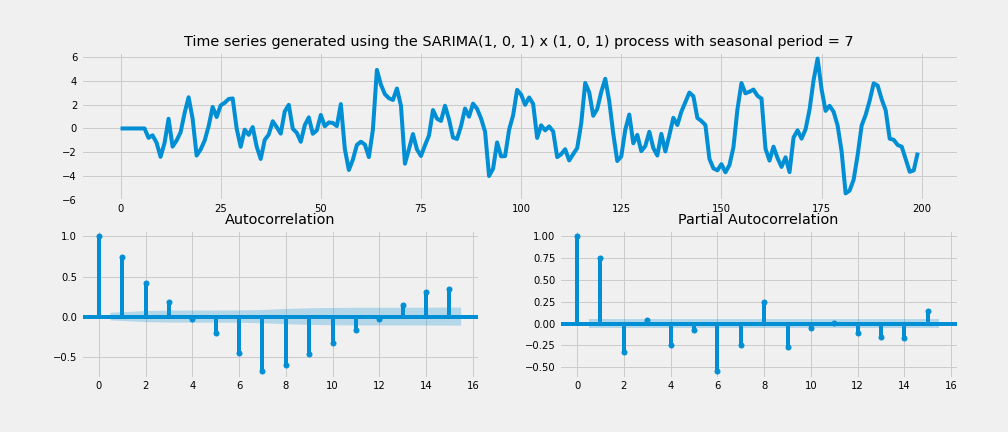
\includegraphics[width=1\textwidth,height=0.5\textwidth]{figures/chapter_03/sarima_example.png}    
\caption{The SARIMA(1, 0, 1) $\times$ (1, 0, 1$)_7$ process example with its ACF and PACF: $\phi_1 = 0.5,\Phi_1 = -0.4, \theta_0 = 0.4, \Theta_1 = -0.3$}    \label{fig:sarima_1_1_1_example}    
\end{figure}

\subsubsection{Example of the seasonal ARIMA time series}

Figure \ref{fig:sarima_1_1_1_example} demonstrates an example of the time series generated by the process denoted as SARIMA(1, 0, 1) $\times$ (1, 0, 1$)_7$. The ACF shows the most expressive autocorrelation at lags 1 and 7. We can also see that the pattern typical for AR processes takes its place not only after lag 1 but after lag 7. The PACF demonstrates correlation at lags 1 and 6.

According to this example, we can guess the possible seasonal period of the time series. However, estimation of the orders of the AR and MA parts is not a simple task.

\subsection{(S)ARIMA model building}

The (S)ARIMA model building consists of several steps. In Shumway et al. \cite{shumway2011} we found that it is possible to specify the following pipeline:
\begin{enumerate}
    \item plotting the data
    \item possible transforming the data
    \item identifying the order of the possible model
    \item parameter estimation
    \item diagnostics
    \item model choice
\end{enumerate}
The first step is common for every data analyst task. It is necessary to visualize the original data to create a list of future actions.

The second step means that sometimes we need to apply some data transformations. For example, if the variance of data increases over time, it will need some manipulations to stabilize the process (for example, \textbf{Box-Cox transformation} or some basic such as \textbf{logarithmic} \cite{osborne2010}). 

After a suitable data transformation, it is possible to estimate the order of the model. In other words, the estimation of general $p, d, q$ orders and seasonal $P, D, Q$. At the beginning of such a process, we need to estimate $d$ and $D$. We can perform differencing, after which we can look at the form of the obtained time series. The ACF and PACF could also be helpful. After $d$ and $D$, we can try to guess the order of the general and seasonal AR and MA components. The curtain estimation could not be possible at all, so we need to find at least approximately suitable values.

The following step implies model fitting. This can be done in a variety of ways. However, in this section we will introduce the \textit{maximum likelihood estimation} (MLE) method \cite{Hyndman2018}. In essence, we need to find parameters, which will maximize the probability of obtaining the original data with the given process. In case of (S)ARIMA it means the minimization of
\begin{equation}
    \sum_{t=1}^{T} \varepsilon_t = Y_t - \hat{Y_t},
\end{equation}
where T is the number of timestamps in historical data, $e_t$ is a residual (introduced, for example, in Equation \ref{eq_additive_model} and Equation \ref{eq_multiplicative_model}) at timestamp $t$, $Y_t$ is the value of the observed variable $Y$ at timestamp $t$, and $\hat{Y_t}$ is the estimated value of the $Y$ at timestamp $t$. It is also possible to coordinate the estimation process using the Akaike information criterion or the Bayesian information criterion.

Finally, we need to perform \textit{residual analysis}, that will be introduced in the practical part of this thesis. It will help us to measure the presence or absence of factors that influence our data but not described by our model (this step is also important for the Prophet model). 

After doing all this, we can start forecasting using our model.

\subsection{Forecasting using the (S)ARIMA model}

In essence, the forecasting with (S)ARIMA model can be shortly explained by a short sequence of actions \cite{Hyndman2018}. 

First, we need to rewrite the model equation for $Y_{T+h}$, where $T$ is the index of the most recent timestamp in the history and $h = 1, 2, \ldots$ is the index of the forecasted timestamp. While forecasting, we need to replace future observations with their forecasts, future errors with zero, and past errors with the corresponding model residuals. The confidential intervals for the forecast are computed according to the methods used in the curtain implementation of the (S)ARIMA model.

\subsection{Summary}

During the theoretical research, we discovered that the ARIMA and SARIMA models (with suitable parameters) can be used to predict the evolution of the COVID-19 pandemic processes. Various studies and researches introduced in at the beginning of this chapter confirm that.

This find, in conjunction with the properties of this kind of statistical models, led us to the fact that it would be a strong choice for modeling pandemic processes and comparation with the Facebook Prophet model.

\hypertarget{ch3}{\chapter{Application of selected statistical models on COVID-19 related time series}}

This chapter aims at the practical application of the statistical models introduced in Chapter \hyperlink{ch2}{2} in the context of modeling time series related to the COVID-19 pandemic in the Czech Republic.

\section{Data}

One of the most determining steps in data analysis is the searching, selection, and preparation of reliable data.

\subsection{Data sources}

The main practical goal of this thesis is to perform an analysis of time series generated by different processes related to the COVID-19 pandemic in the Czech Republic. According to this fact, the fundamental data source for this work is the official website created in association with the Ministry of Health of the Czech Republic with information about it \cite{covidczdata}.

\subsection{Data selection}

After inspection of the available data and exploring different articles that aim at the modeling of COVID-19 pandemic time series in various countries all around the world, we decided to select the time series that describe \textbf{the cumulative number of people infected}, \textbf{the cumulative number of people cured}, \textbf{the cumulative number of people dead}, and \textbf{the number of active cases}.

All selected data frames were last updated on May 4, 2021 and store measurements obtained from March 1, 2020. 

\subsection{Data preparation}

All data were obtained from an official and reliable web source. Thus, there were no consistency data problems such as missing or invalid values. However, there was no time series with information about the active cases ($A$), so it was aggregated from time series that describe the number of people infected ($I$), cured ($C$), and dead ($D$) using the following formula
\begin{equation}
    A = I - C - D.
\end{equation}
After doing that, it is necessary to transform each data frame into a form compatible with the Facebook Prophet model. Table \ref{tab:cum_inf_example_table} demonstrates the time series with information about the number of people infected daily in its final form.

\begin{table}[!ht]
    \centering
    \begin{tabular}{|p{3cm}|p{3cm}|}
    \hline
     \multicolumn{2}{|c|}{\textbf{Cumulative number of people infected
     }} \\
    \hline
    \textbf{ds} & \textbf{y}\\
    \hline
    2020-03-01 & 3\\
    \hline
	2020-03-02 & 3\\
	\hline
	2020-03-03 & 5\\
	\hline
	2020-03-04 & 6\\
	\hline
    2020-03-05 & 9\\
 \hline
\end{tabular}
    \caption{Final form of the data frame with information about cumulative amount of people infected.}
    \label{tab:cum_inf_example_table}
\end{table}

\hypertarget{s3.2}{\section{Basic analysis of the selected time series}}

After preparing all the selected time series, we need to perform their basic analysis to 
\begin{itemize}
    \item find some interesting phenomena, possible seasonal or cyclic patterns,
    \item estimate the order of future SARIMA models,
    \item perform basic statistical testing (stationarity tests).
\end{itemize}
Now, we can perform an analysis of each time series individually.

\begin{figure}[!ht]
\centering
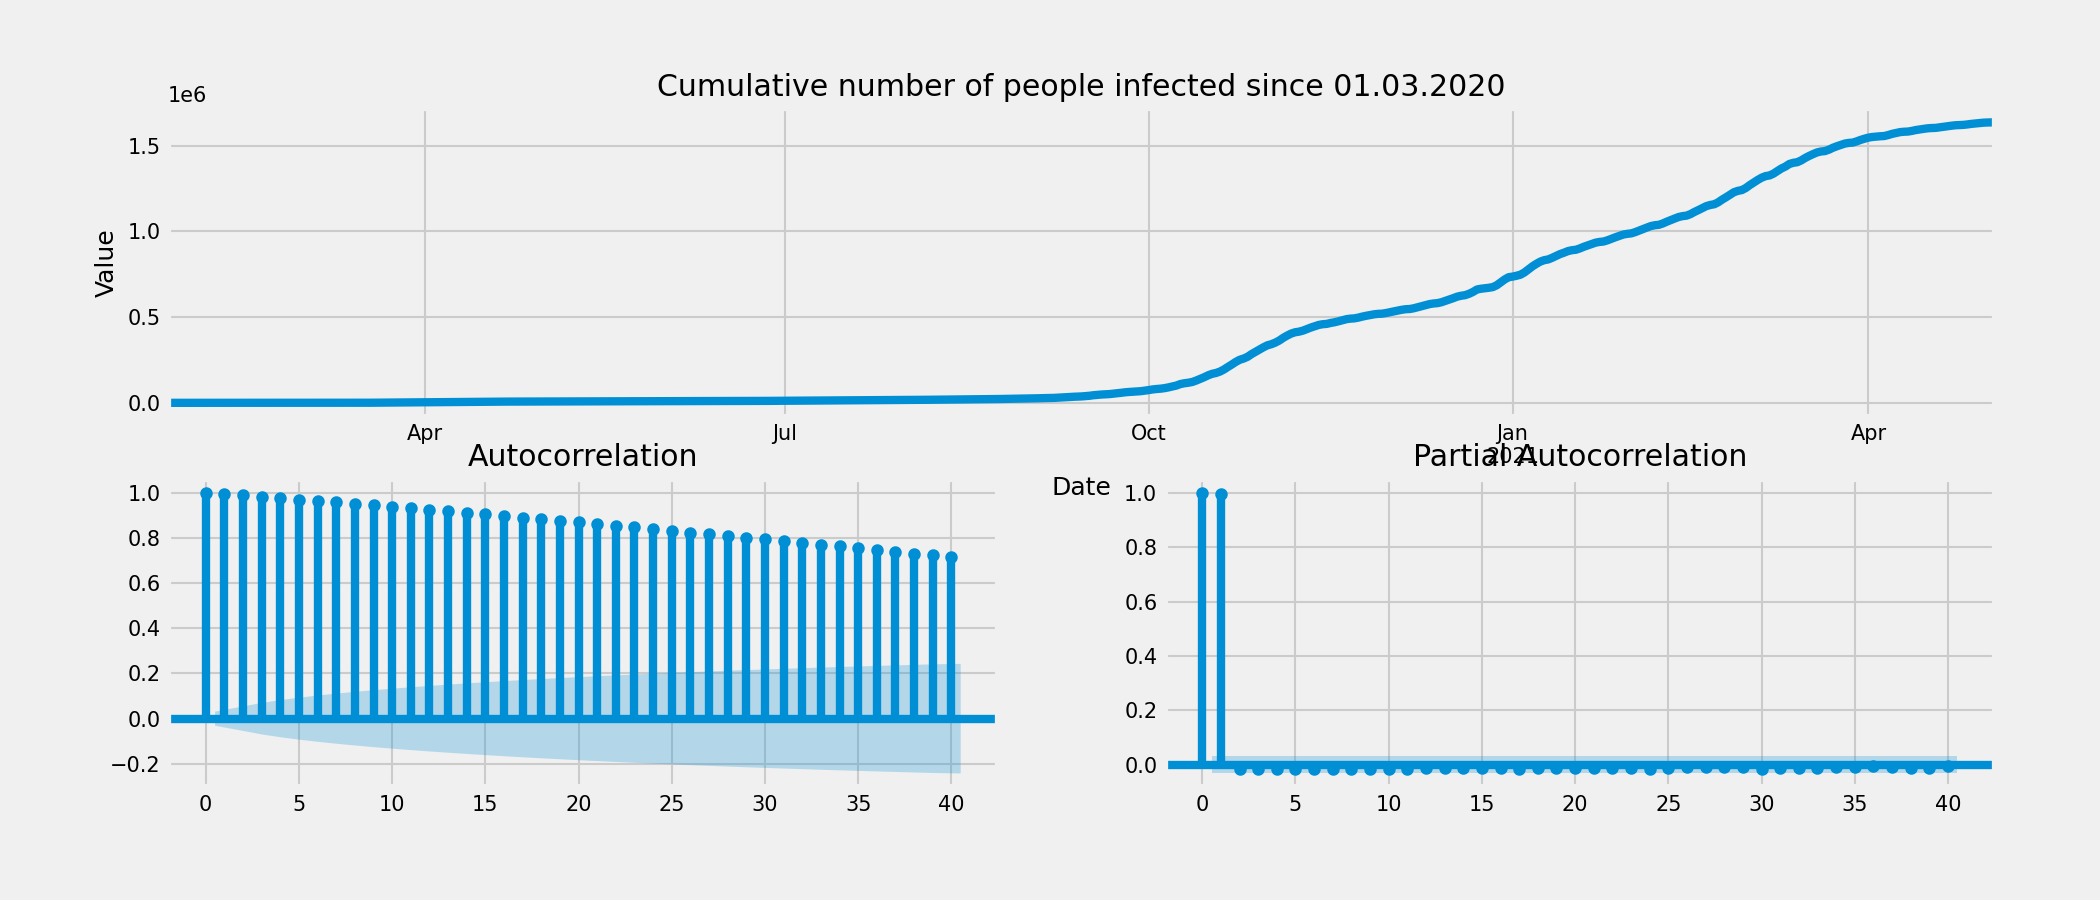
\includegraphics[width=1\textwidth, height=0.35\textwidth]{figures/chapter_04/original_ts/ts_orig_infected.png}
\caption{The cumulative number of people infected in Czech Republic time series with the corresponding ACF and PACF.}
\label{fig:orin_infected}
\end{figure}
\begin{figure}[!htb]
  \centering
  \subfloat[a][The cumulative number of people infected time series after differencing at lag 1.]{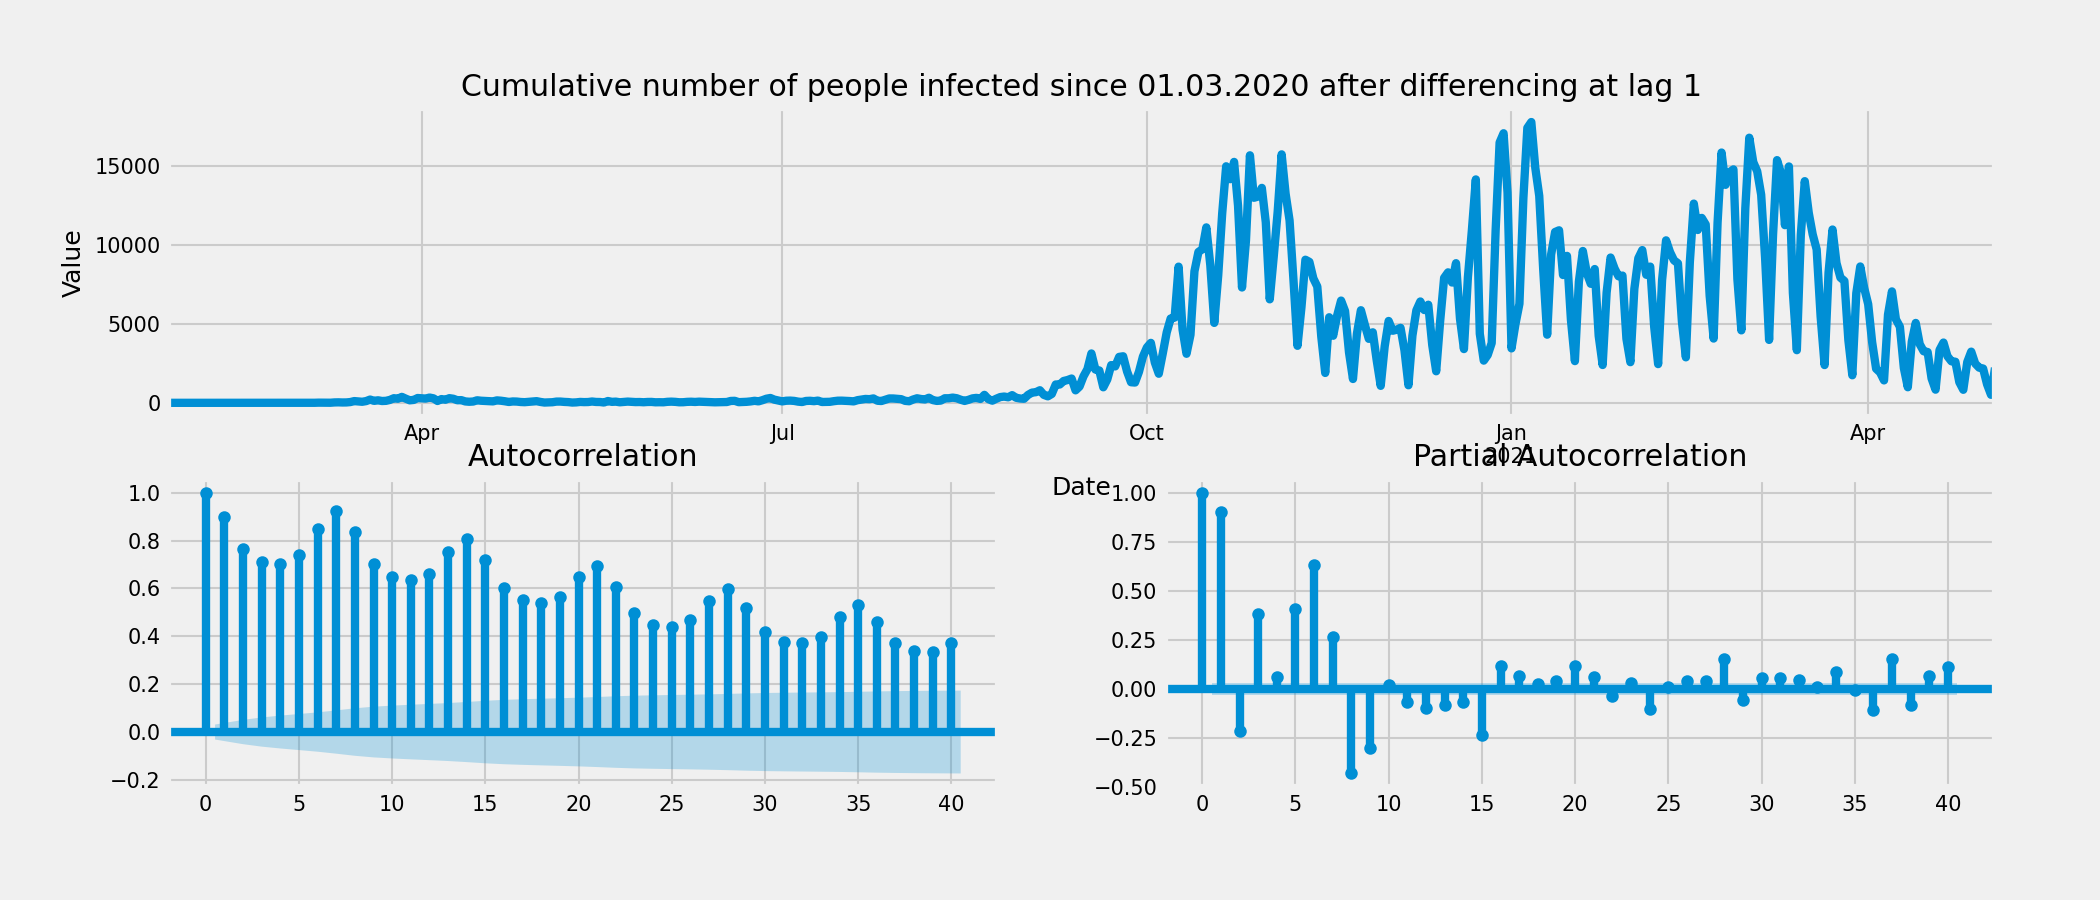
\includegraphics[width=1\textwidth, height=0.3\textwidth]{figures/chapter_04/infected_ts/ts_diff_infected.png}
  \label{fig:infected_diff}} \\
  \subfloat[b][The cumulative number of people infected time series after double differencing at lag 1.]{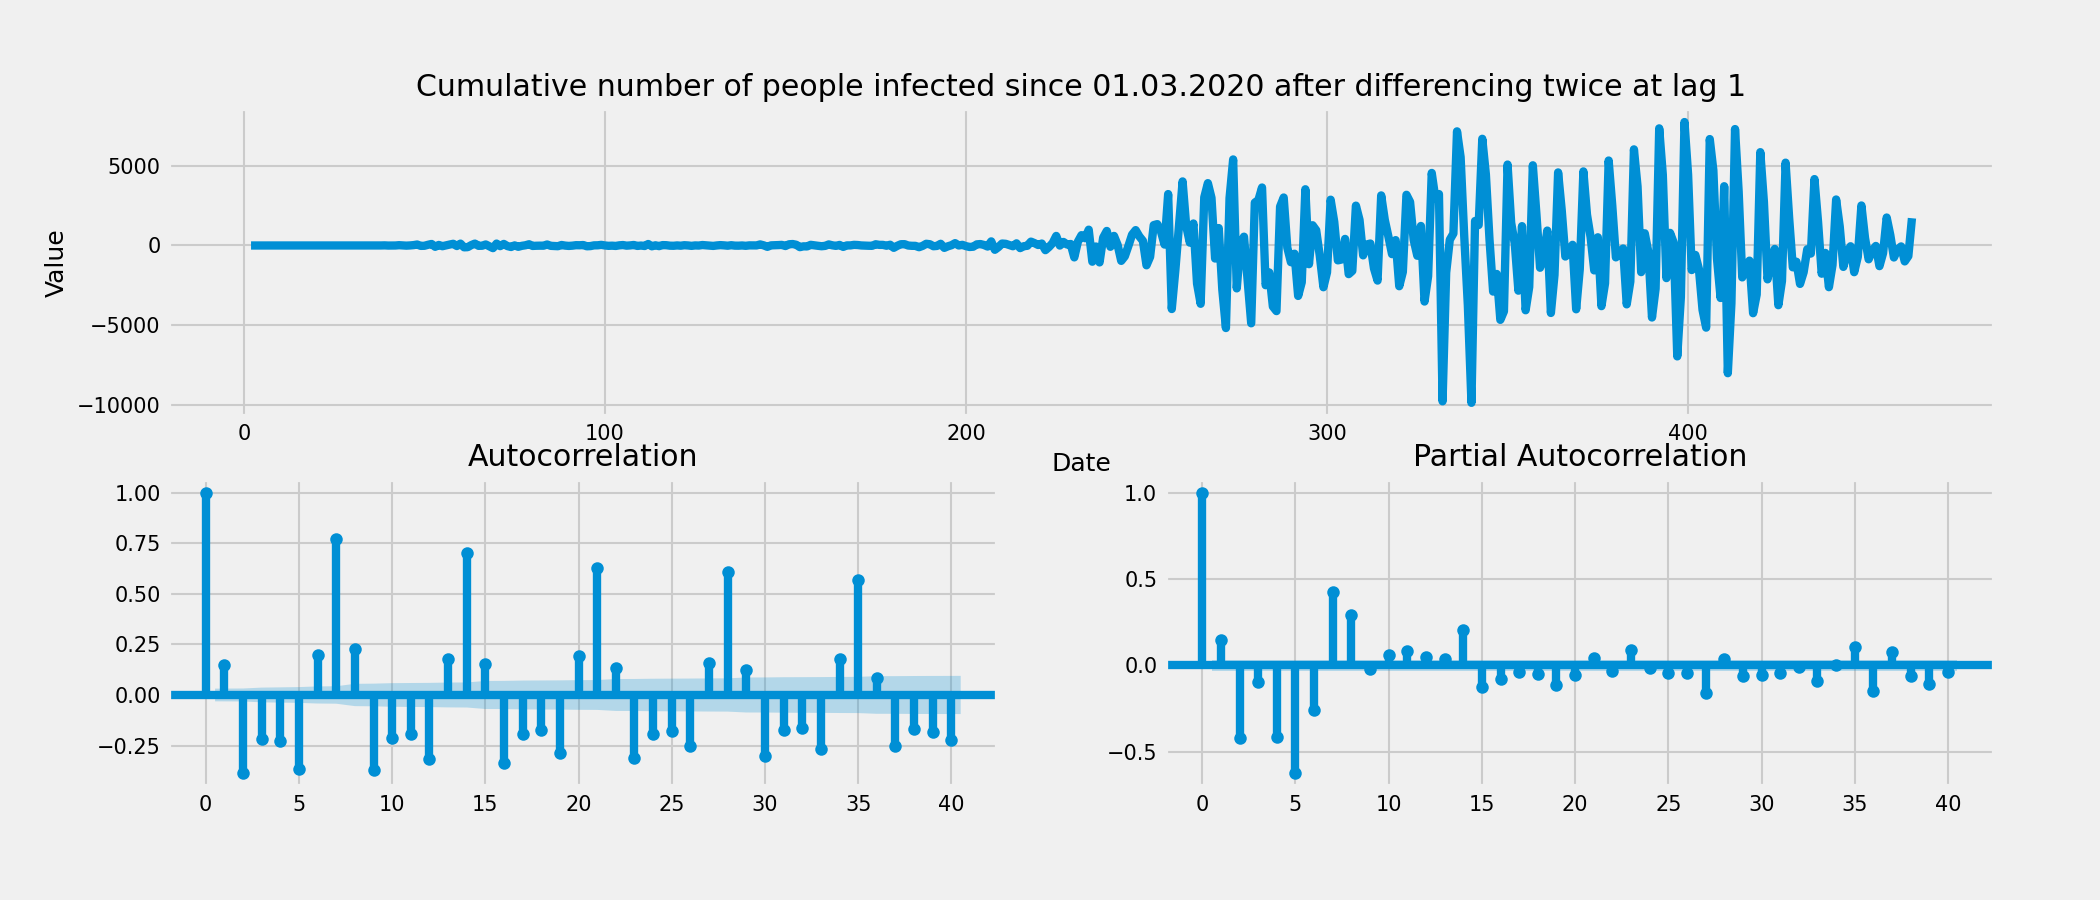
\includegraphics[width=1\textwidth, height=0.3\textwidth]{figures/chapter_04/infected_ts/ts_diff1_1_infected.png}
  \label{fig:infected_diff_1_1}} \\
  \subfloat[c][The cumulative number of people infected time series after differencing at lag 1 and 7.]{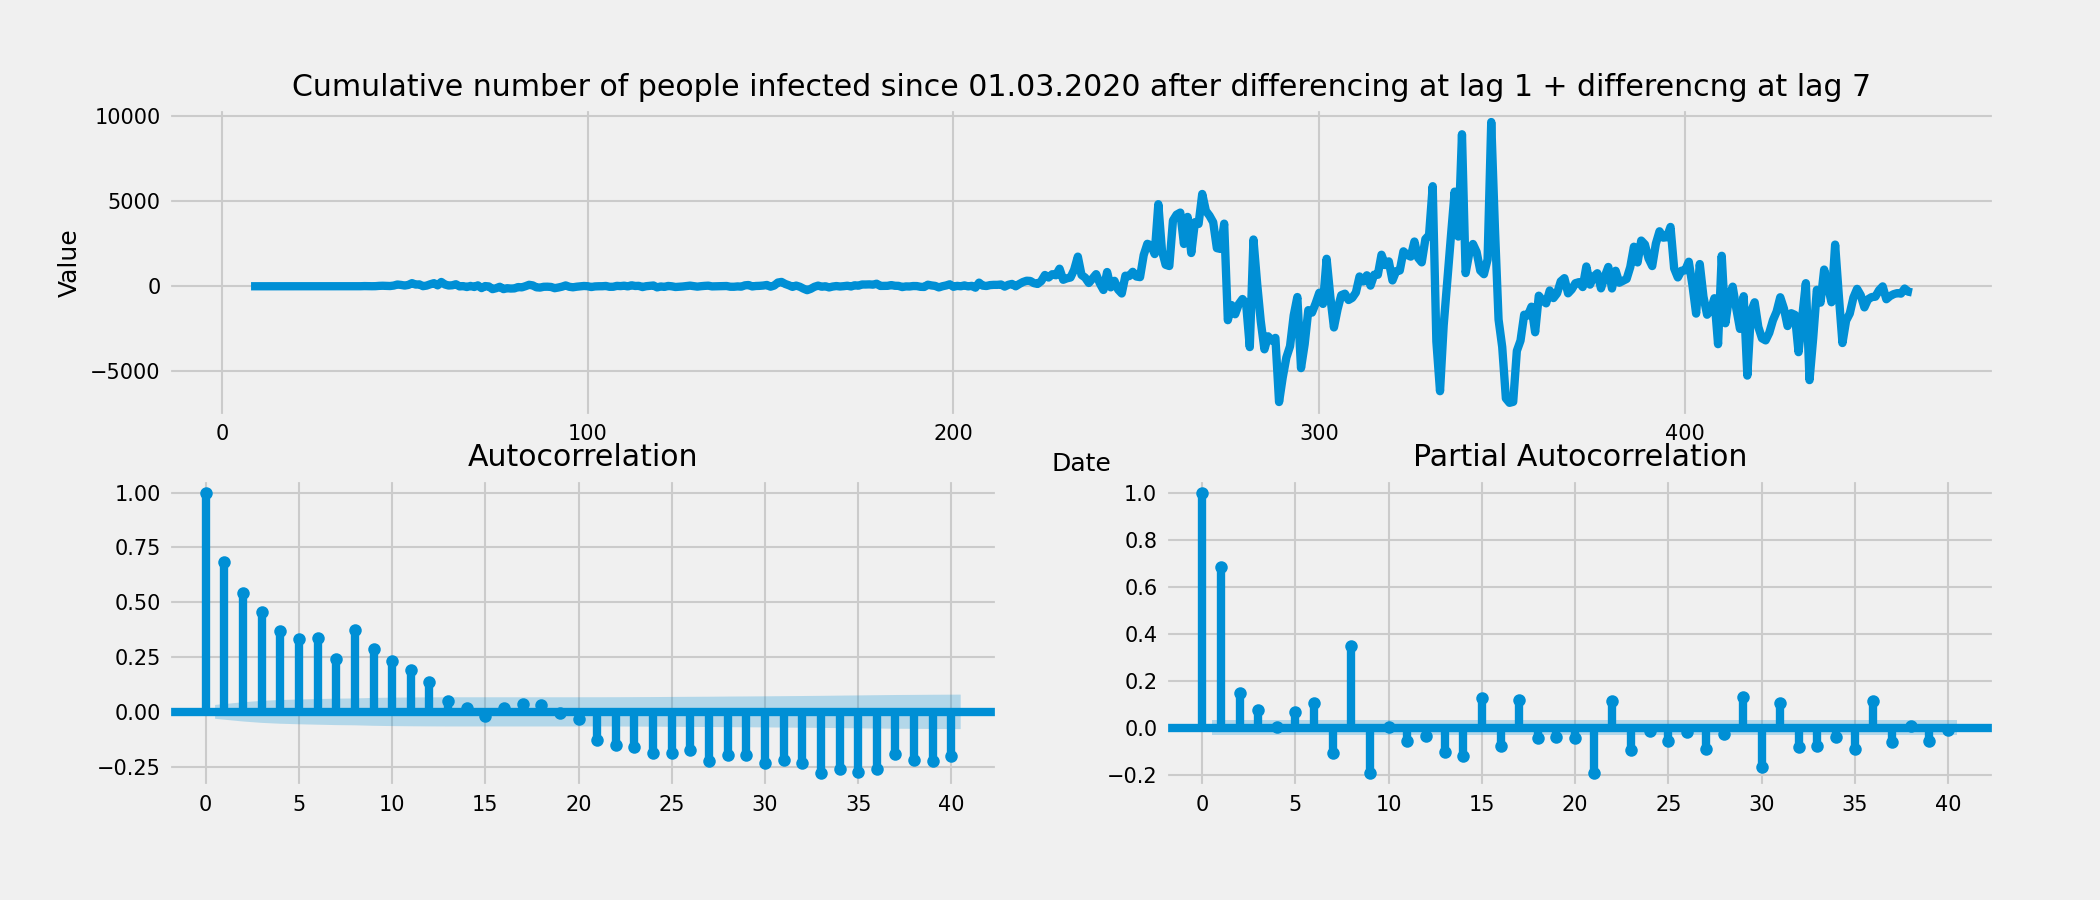
\includegraphics[width=1\textwidth, height=0.3\textwidth]{figures/chapter_04/infected_ts/ts_diff1_7_infected.png}
  \label{fig:infected_diff_1_7}}
  \caption{The cumulative amount of people infected after different differencing sequences with the corresponding ACF and PACF.}
  \label{fig:infected_diff_ex}
\end{figure}

\subsection{Cumulative number of people infected daily time series}

First, we will inspect the cumulative number of people infected time series.

Figure \ref{fig:orin_infected} demonstrates the original time series that describes the cumulative number of people infected daily with the corresponding ACF and PACF. It is clear that this time series is a cumulative sum, so it does not give any valuable information. Thus, we need to perform differencing at lag 1.

Now we can see (Figure \ref{fig:infected_diff}) the following interesting properties of this time series:
\begin{itemize}
    \item There is no interesting activity until the beginning of June. It means that we can drop the first part of the time series during the modeling process.
    \item According to the ACF, there is a global trend (the correlation measure slowly decreases) and weekly seasonality (peaks at lags 7, 14, 21, and so on).
    \item According to the stationarity tests (Table 3.2), this is a nonstationary time series.
\end{itemize}
This leads to the fact that we need to get rid of nonstationarity. However, it is possible in two ways: one more differencing at lag 1 or seasonal differencing at lag 7. 

In Figure \ref{fig:infected_diff_1_1} and Figure \ref{fig:infected_diff_1_7} you can see the time series after double differencing at lag 1 and after one-time differencing at lag 1 and lag 7, respectively. 

In the first case, we got rid of the global trend, but we still have seasonality (significant correlation at lag 7, 14, and so on). Moreover, Table \ref{tab:infected_tests_table} indicates that the time series is now stationary. The ACF shows that the possible seasonal autoregressive order is 1.

In the second case, we got rid of the seasonality. Stationarity tests (Table \ref{tab:infected_tests_table}) indicate that the time series is now stationary. The ACF and PACF show that the possible autoregressive order is 1.

All this information follows that the cumulative number of people infected time series is generated by the process that can be described by SARIMA(1, 2, 0) $\times$ (1, 0, 0$)_7$ or SARIMA(1, 1, 0) $\times$ (1, 1, 0$)_7$ models.

\begin{table}[!ht]
    \centering
    \begin{tabular}{|p{3cm}||p{3cm}| p{3cm}|}
    \hline
    Time series & Dikey-Fuller test p-value & KPSS test p-value\\
    \hline
    Original time series& 0.993501 & 0.010000\\
    \hline
    1x at lag 1 & 0.295332 & 0.010000\\
	\hline
	2x at lag 1 & 0.001123 & 0.100000\\
	\hline
	1x lag 1; 1x at lag 7 & 0.001654 & 0.100000\\
 \hline
\end{tabular}
    \caption{The Cumulative number of people infected: results of the stationarity tests.}
    \label{tab:infected_tests_table}
\end{table}

\subsection{The cumulative number of people cured time series}

Figure \ref{fig:orig_cured} demonstrates the original time series that describes the cumulative number of people cured daily with the corresponding ACF and PACF. Similar to the previous time series, it is a cumulative sum. Thus, we need to perform differencing at lag 1. 

Figure \ref{fig:cured_diff} shows the time series after the first differencing. We can see the global trend and weekly seasonality. The ACF and PACF also demonstrate a slowly decreasing measure of correlation. Additionally, the ACF shows peaks at lags 7, 14, 21, and so on (seasonality). In Table \ref{tab:cured_tests_table} we can find out that this time series is nonstationary, and we need to do one more differencing. 

\begin{table}[!ht]
    \centering
    \begin{tabular}{|p{3cm}||p{3cm}| p{3cm}|}
    \hline
    Time series & Dikey-Fuller test p-value & KPSS test p-value\\
    \hline
    Original time series& 0.928839 & 0.010000\\
	\hline
	1x at lag 1 & 0.120930 & 0.010000\\
	\hline
	2x at lag 1 &  0.000021 & 0.100000\\
	\hline
	1x lag 1; 1x at lag 7 & 0.000027 & 0.100000\\
 \hline
\end{tabular}
    \caption{The Cumulative number of people cured: results of the stationarity tests.}
    \label{tab:cured_tests_table}
\end{table}

\begin{figure}[!htb]
  \centering
  \subfloat[a][The original cumulative number of people cured time series.]{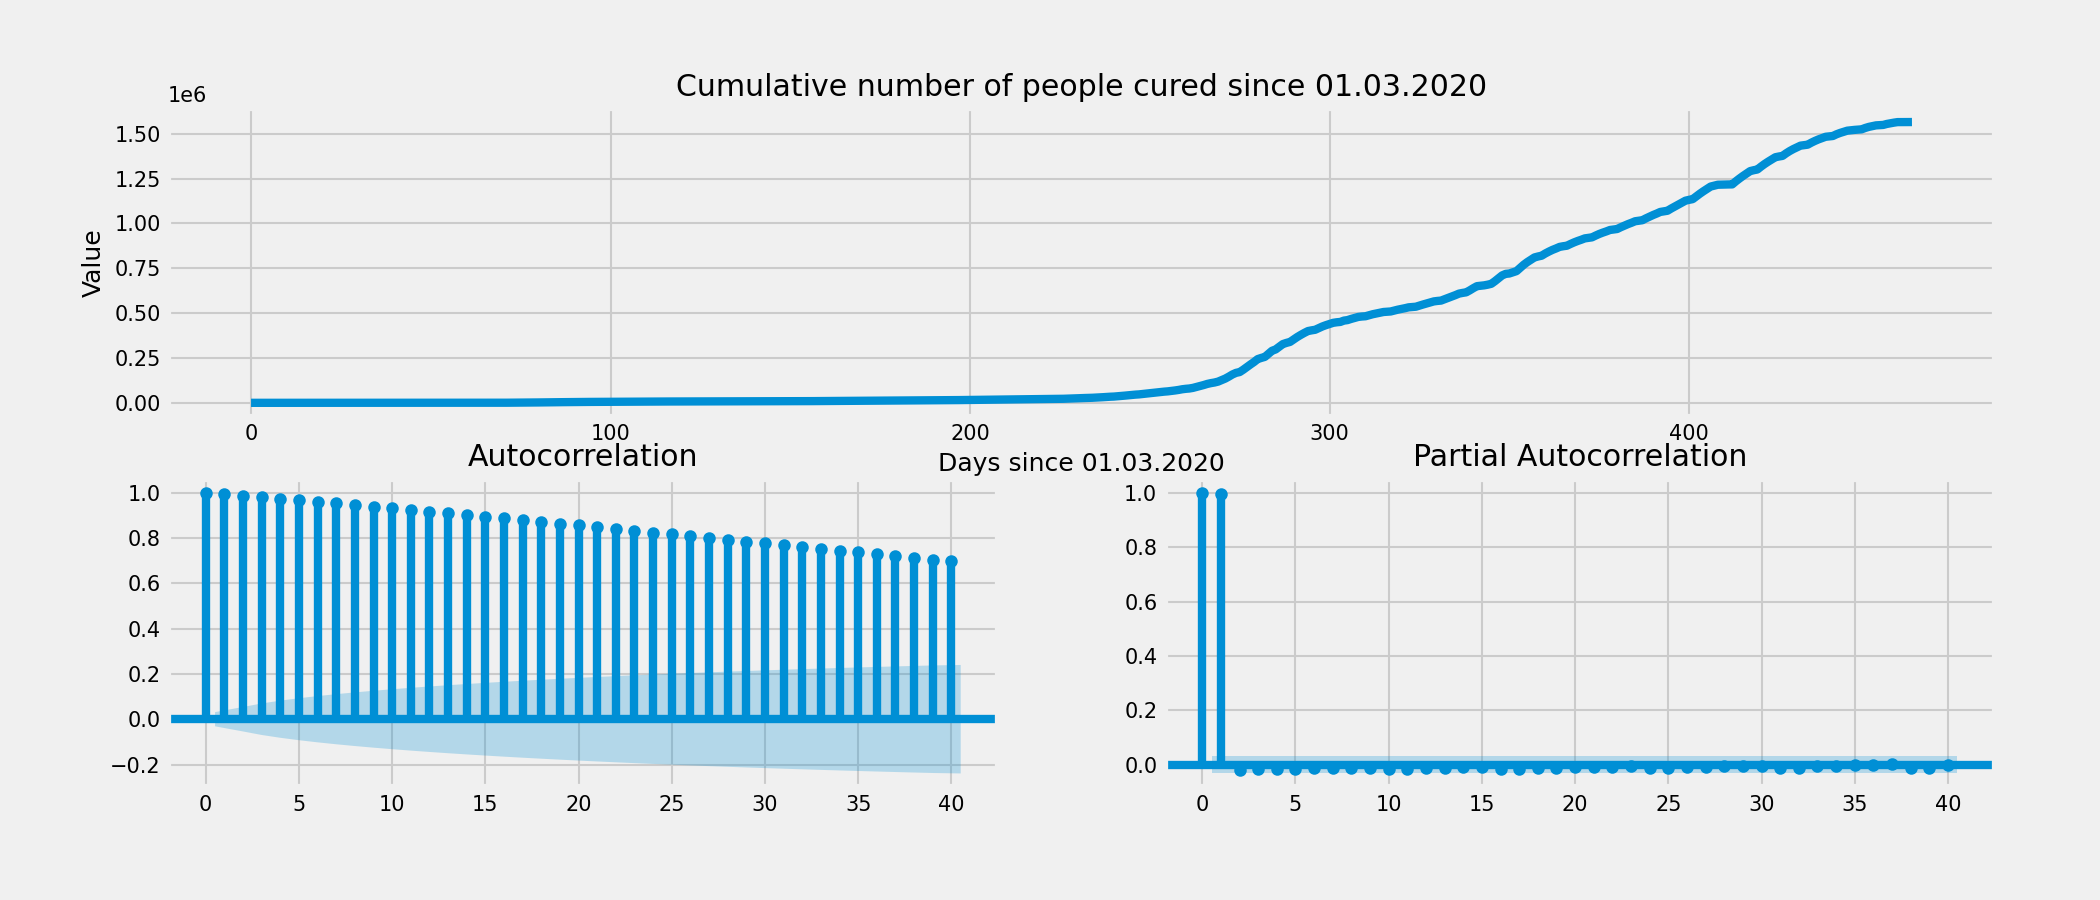
\includegraphics[width=1\textwidth, height=0.28\textwidth]{figures/chapter_04/original_ts/ts_orig_cured.png}
  \label{fig:orig_cured}} \\
  \subfloat[b][The cumulative number of people cured time series after differencing at lag 1.]{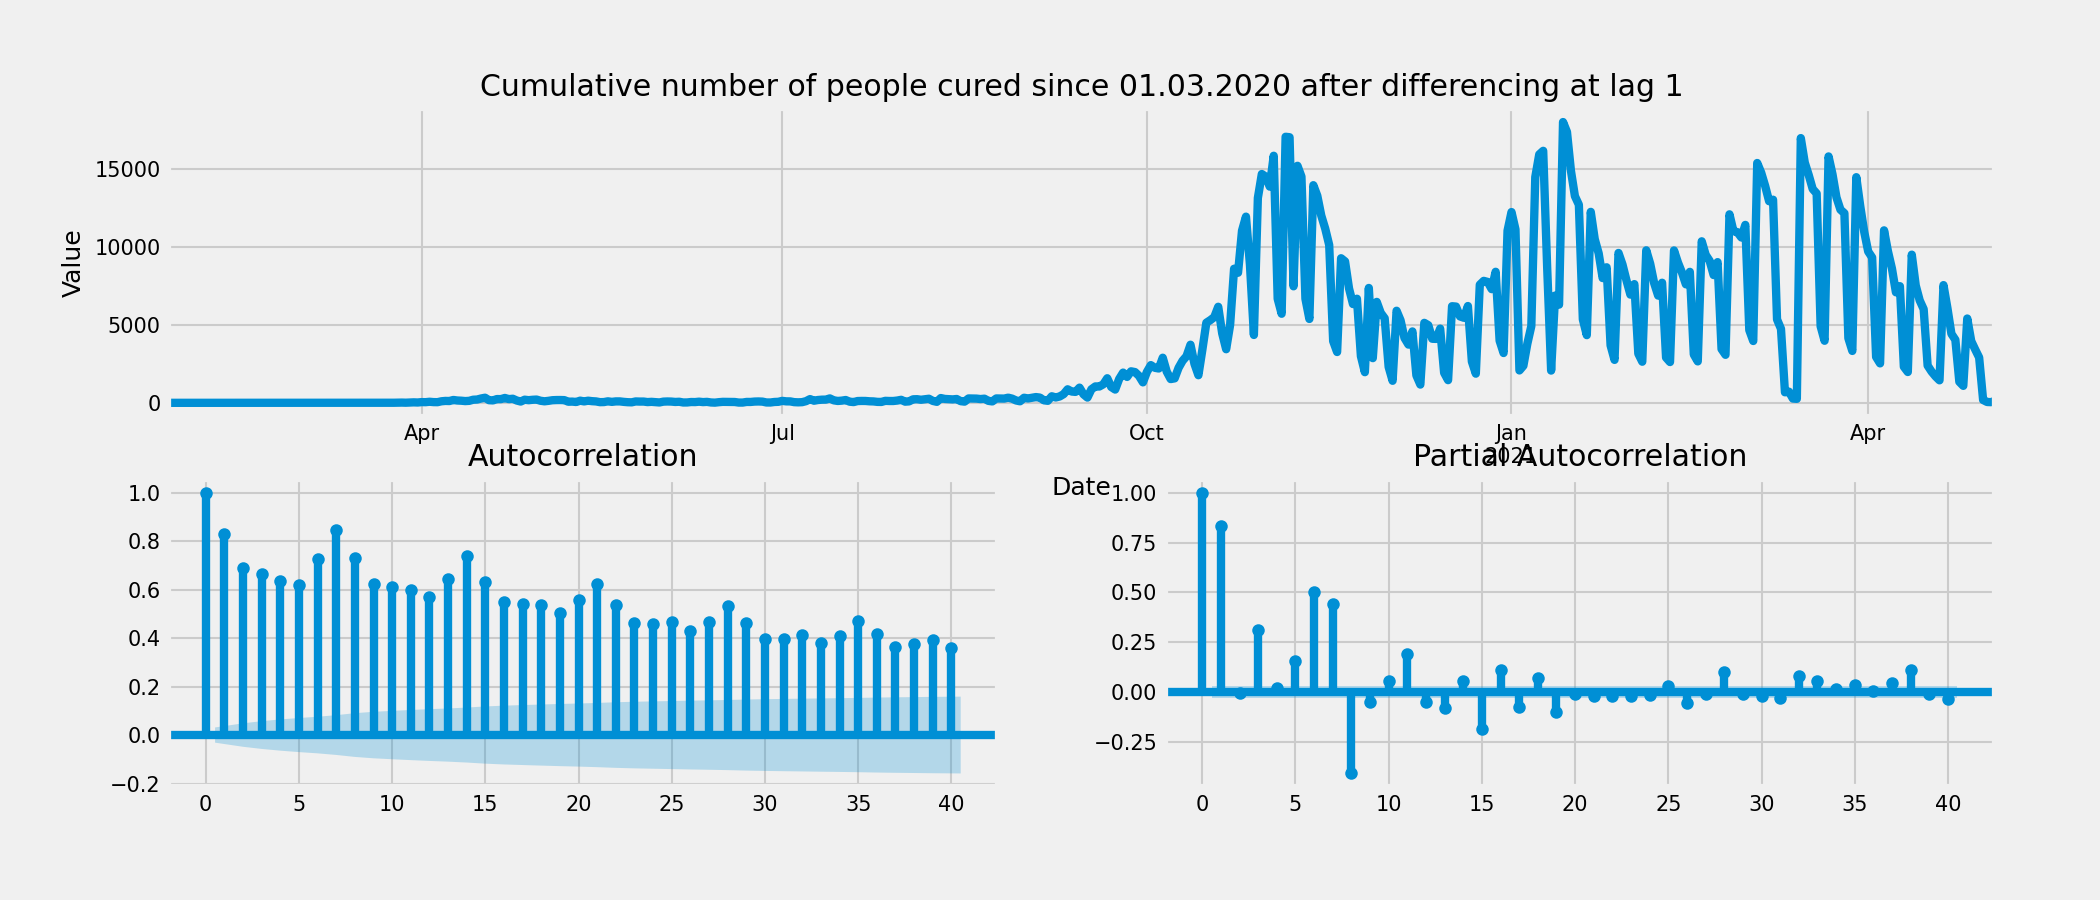
\includegraphics[width=1\textwidth, height=0.28\textwidth]{figures/chapter_04/cured_ts/ts_diff_cured.png}
  \label{fig:cured_diff}} \\
  \subfloat[c][The cumulative number of people cured time series after double differencing at lag 1.]{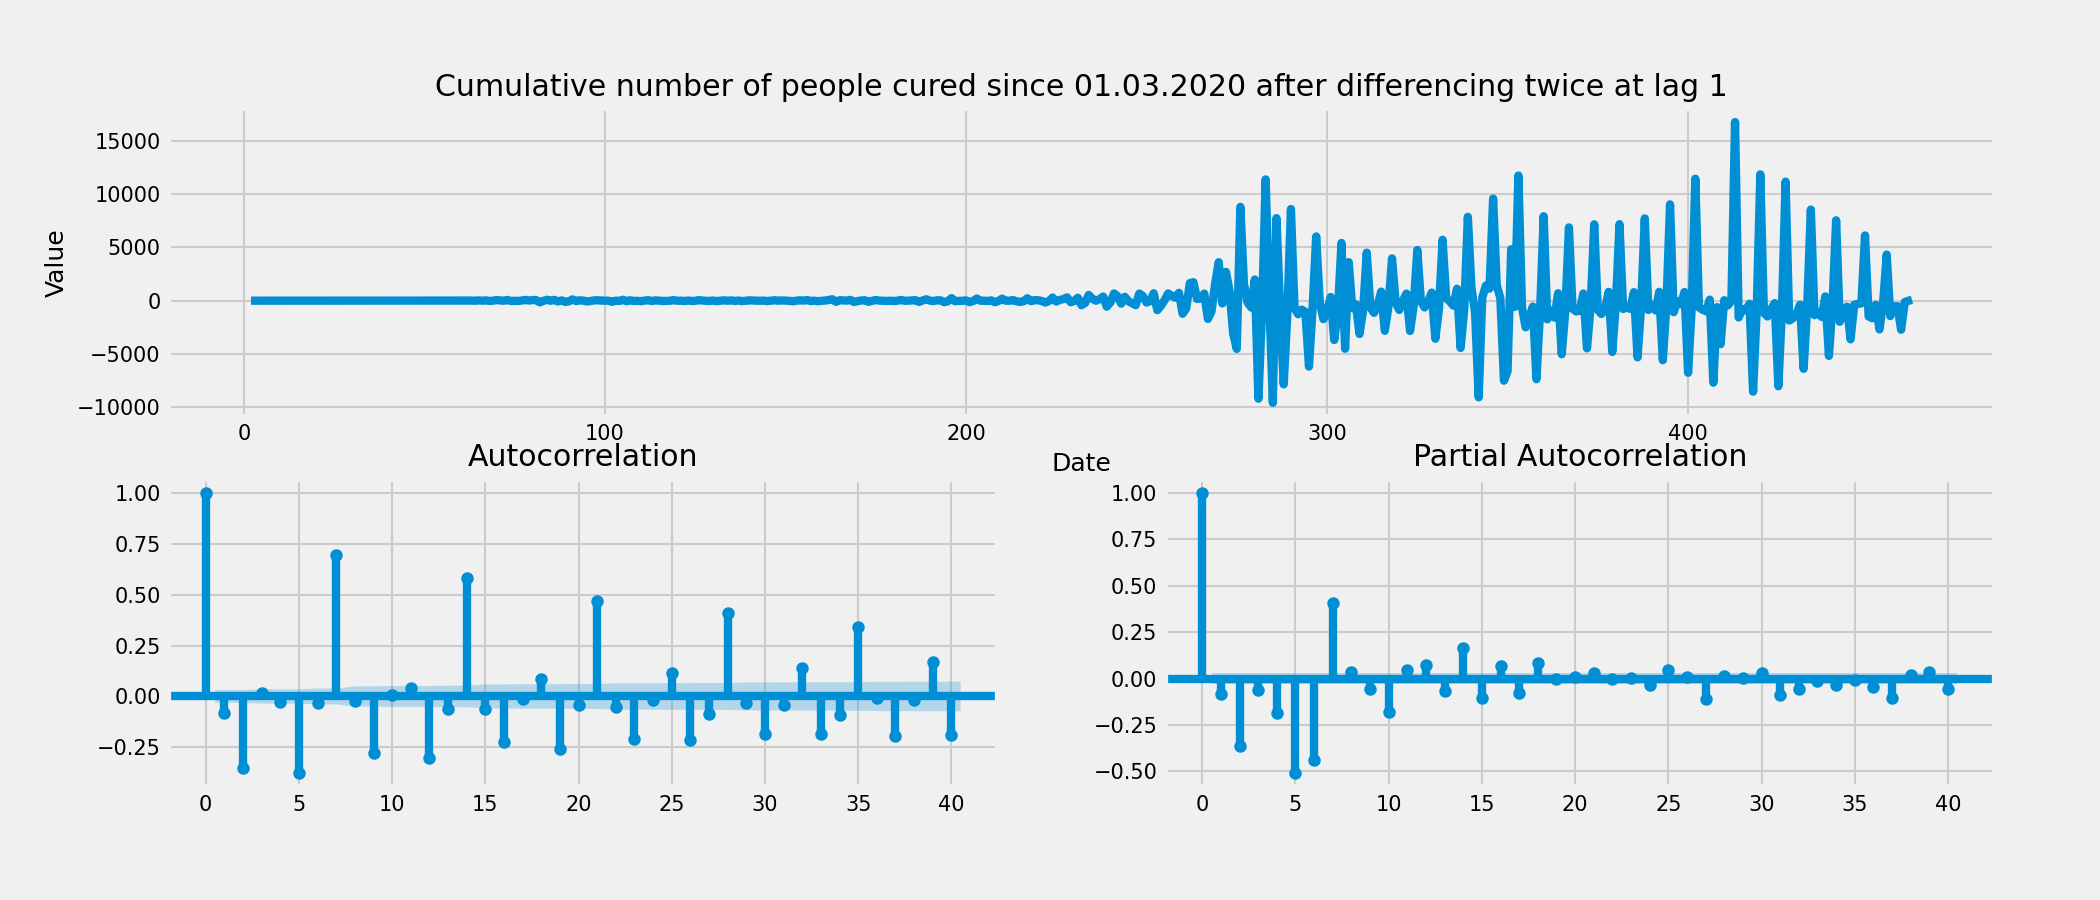
\includegraphics[width=1\textwidth, height=0.28\textwidth]{figures/chapter_04/cured_ts/ts_diff1_1_cured.png}
  \label{fig:cured_diff_1_1}} \\
  \subfloat[d][The cumulative number of people cured time series after differencing at lag 1 and 7.]{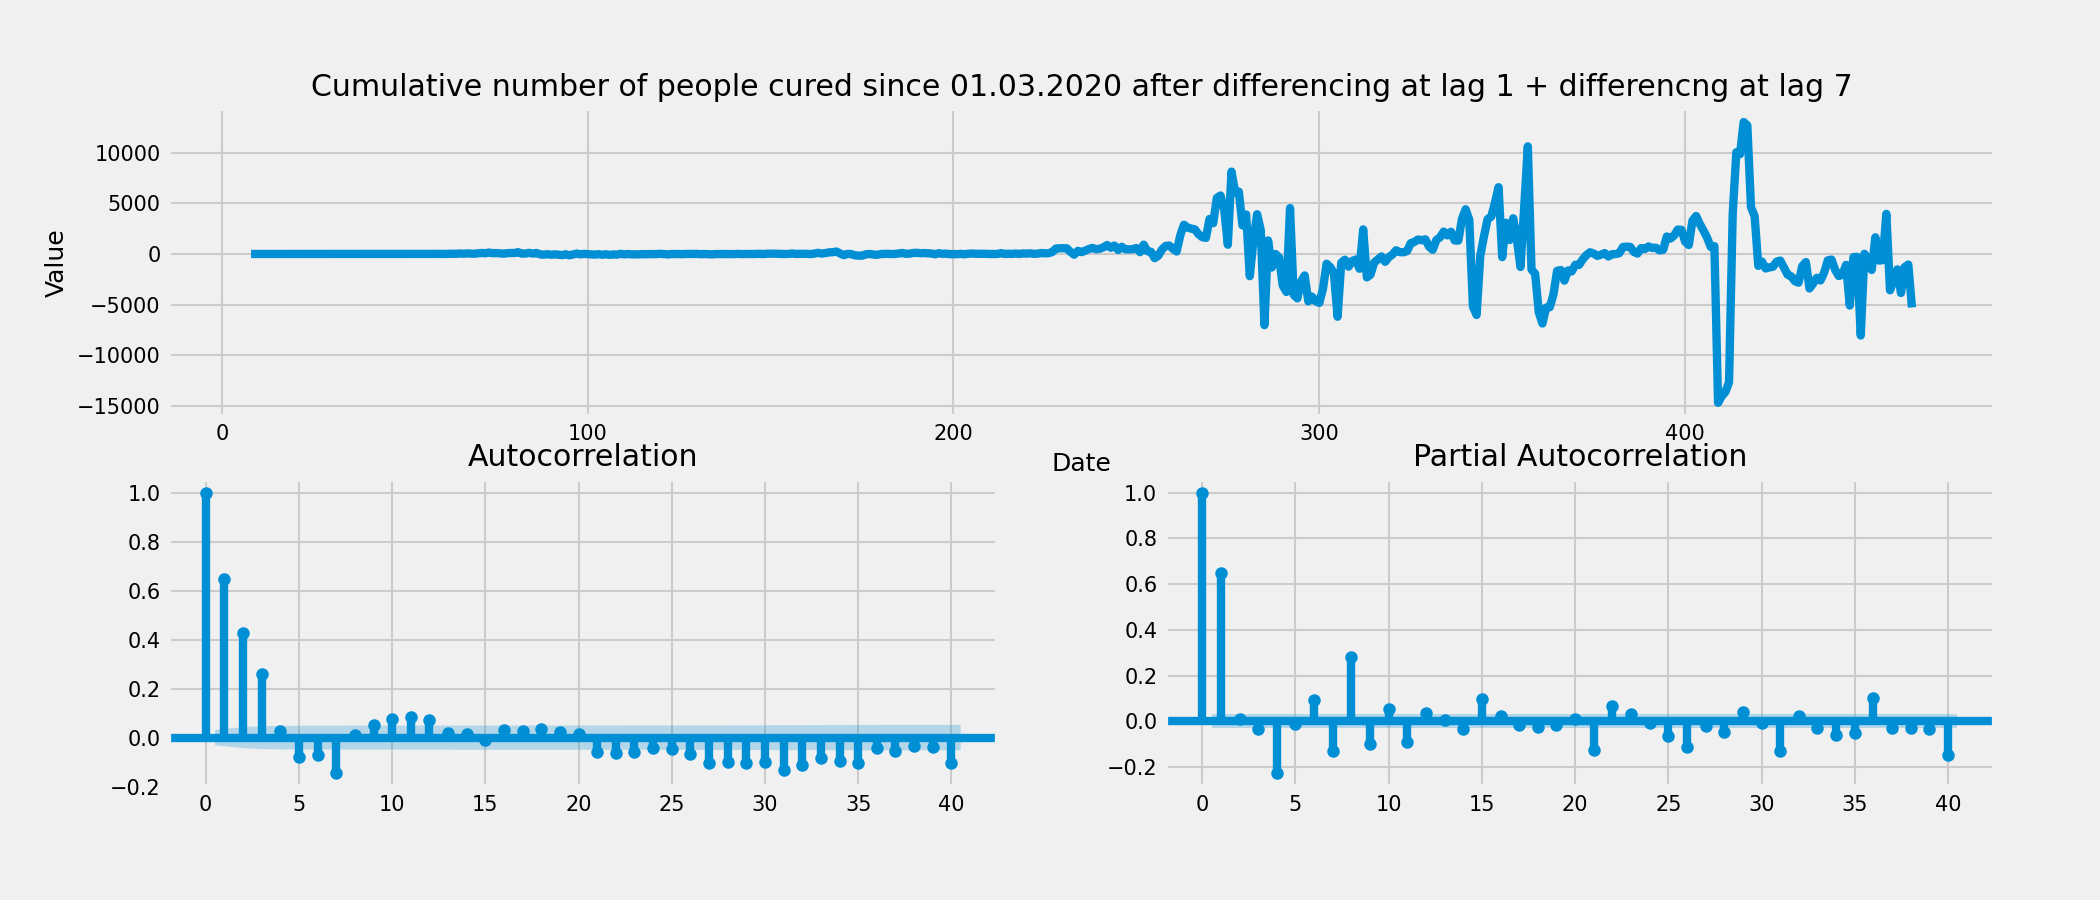
\includegraphics[width=1\textwidth, height=0.28\textwidth]{figures/chapter_04/cured_ts/ts_diff1_7_cured.png}
  \label{fig:cured_diff_1_7}}
  \caption{The cumulative amount of people cured after different differencing sequences with the corresponding ACF and PACF.}
  \label{fig:cured_diff_ex}
\end{figure}

As in the case of the cumulative number of people infected, we can do this by one more differencing at lag 1 or lag 7 (seasonal differencing).

After the second differencing at lag 1 (Figure \ref{fig:cured_diff_1_1}), the time series is now stationary (Table \ref{tab:cured_tests_table}). There is also a considerable value of the ACF at lag 7, 14, 21 (seasonality). This fact indicates that the potential order of the seasonal autoregressive part is 1.

After differencing at lag 7 (Figure \ref{fig:cured_diff_1_7}), the time series is now also stationary (Table \ref{tab:cured_tests_table}). We got rid of seasonality. The ACF shows a fast decrease, and the PACF shows a drop after the first lag, so we can say that the order of the general autoregressive component can be equal to 1. 

Based on the above, the cumulative number of people cured time series is possibly generated by the process that can be described by SARIMA(1, 2, 0) $\times$ (1, 0, 0$)_7$ or SARIMA(1, 1, 0) $\times$ (1, 1, 0$)_7$ models.

\subsection{Cumulative number of people dead time series}

Originally, the third selected time series is also a cumulative sum. After the first differencing at lag 1, it is clear that it still has the global trend, but no seasonality at all. 

Figure \ref{fig:dead_diff} demonstrates that after the second difference at lag 1, we got rid of the global trend. 

It is clear that there are no interesting phenomena in the data until the beginning of June (we can get rid of these measurements in the future). This period is also fundamentally different from the rest of the time series.

\begin{table}[!ht]
    \centering
    \begin{tabular}{|p{3cm}||p{3cm}| p{3cm}|}
    \hline
    Time series & Dikey-Fuller test p-value & KPSS test p-value\\
    \hline
    Original time series& 0.951460 & 0.010000\\
	\hline
	1x at lag 1 & 0.229294 & 0.010000\\
	\hline
	2x at lag 1 &  0.003183 & 0.030002\\
	\hline
	2x at lag 1 + Box-Cox &  0.035768 & 0.100000\\
	\hline
	2x at lag 1 + drop &  0.021909 & 0.061904\\
 \hline
\end{tabular}
    \caption{The Cumulative number of people dead: results of the stationarity tests.}
    \label{tab:dead_tests_table}
\end{table}

The ACF and PACF contain the drop after lag 1. It can indicate the absence of the autoregressive component, but the moving average order can be equal to 1. However, stationarity tests both reject the null hypothesis (Table \ref{tab:dead_tests_table}). It means that the data are likely heteroscedastic and may have structural changes over time.

\begin{figure}[!htb]
  \centering
  \subfloat[a][The original cumulative number of people dead time series.]{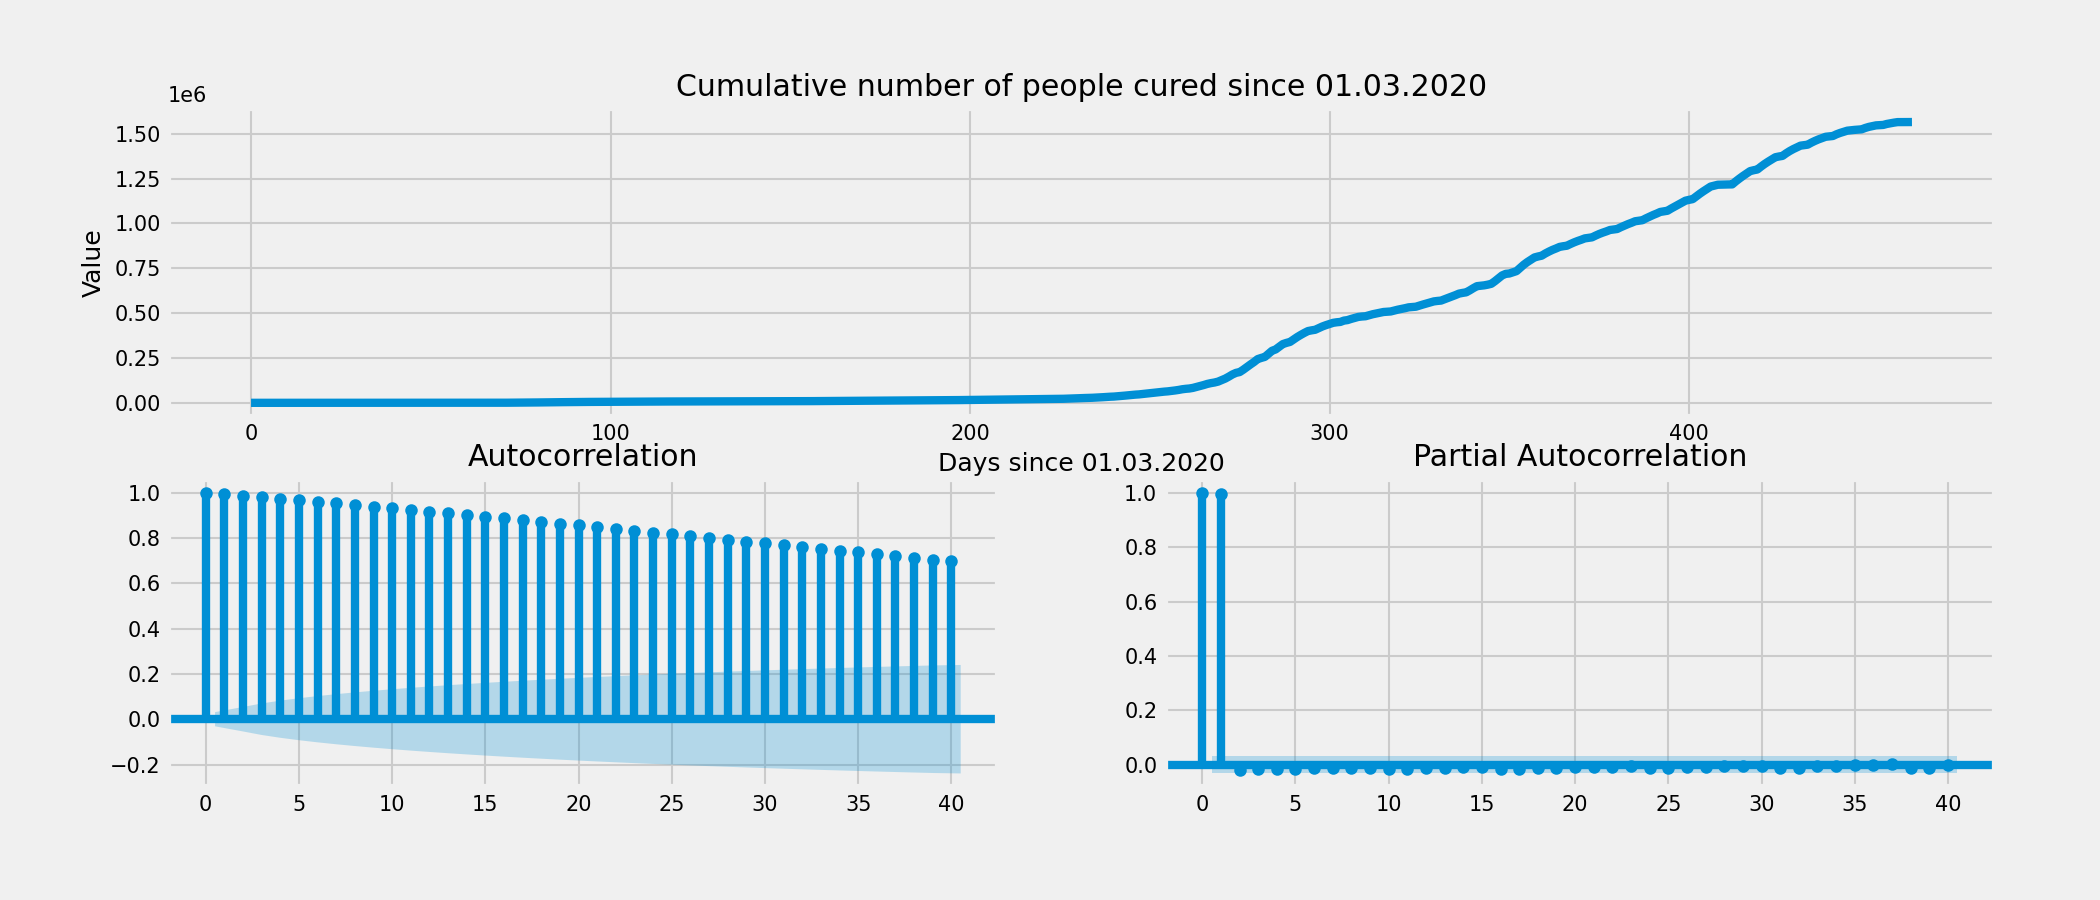
\includegraphics[width=1\textwidth, height=0.3\textwidth]{figures/chapter_04/original_ts/ts_orig_cured.png}
  \label{fig:orig_dead}} \\
  \subfloat[b][The cumulative number of people dead time series after differencing at lag 1.]{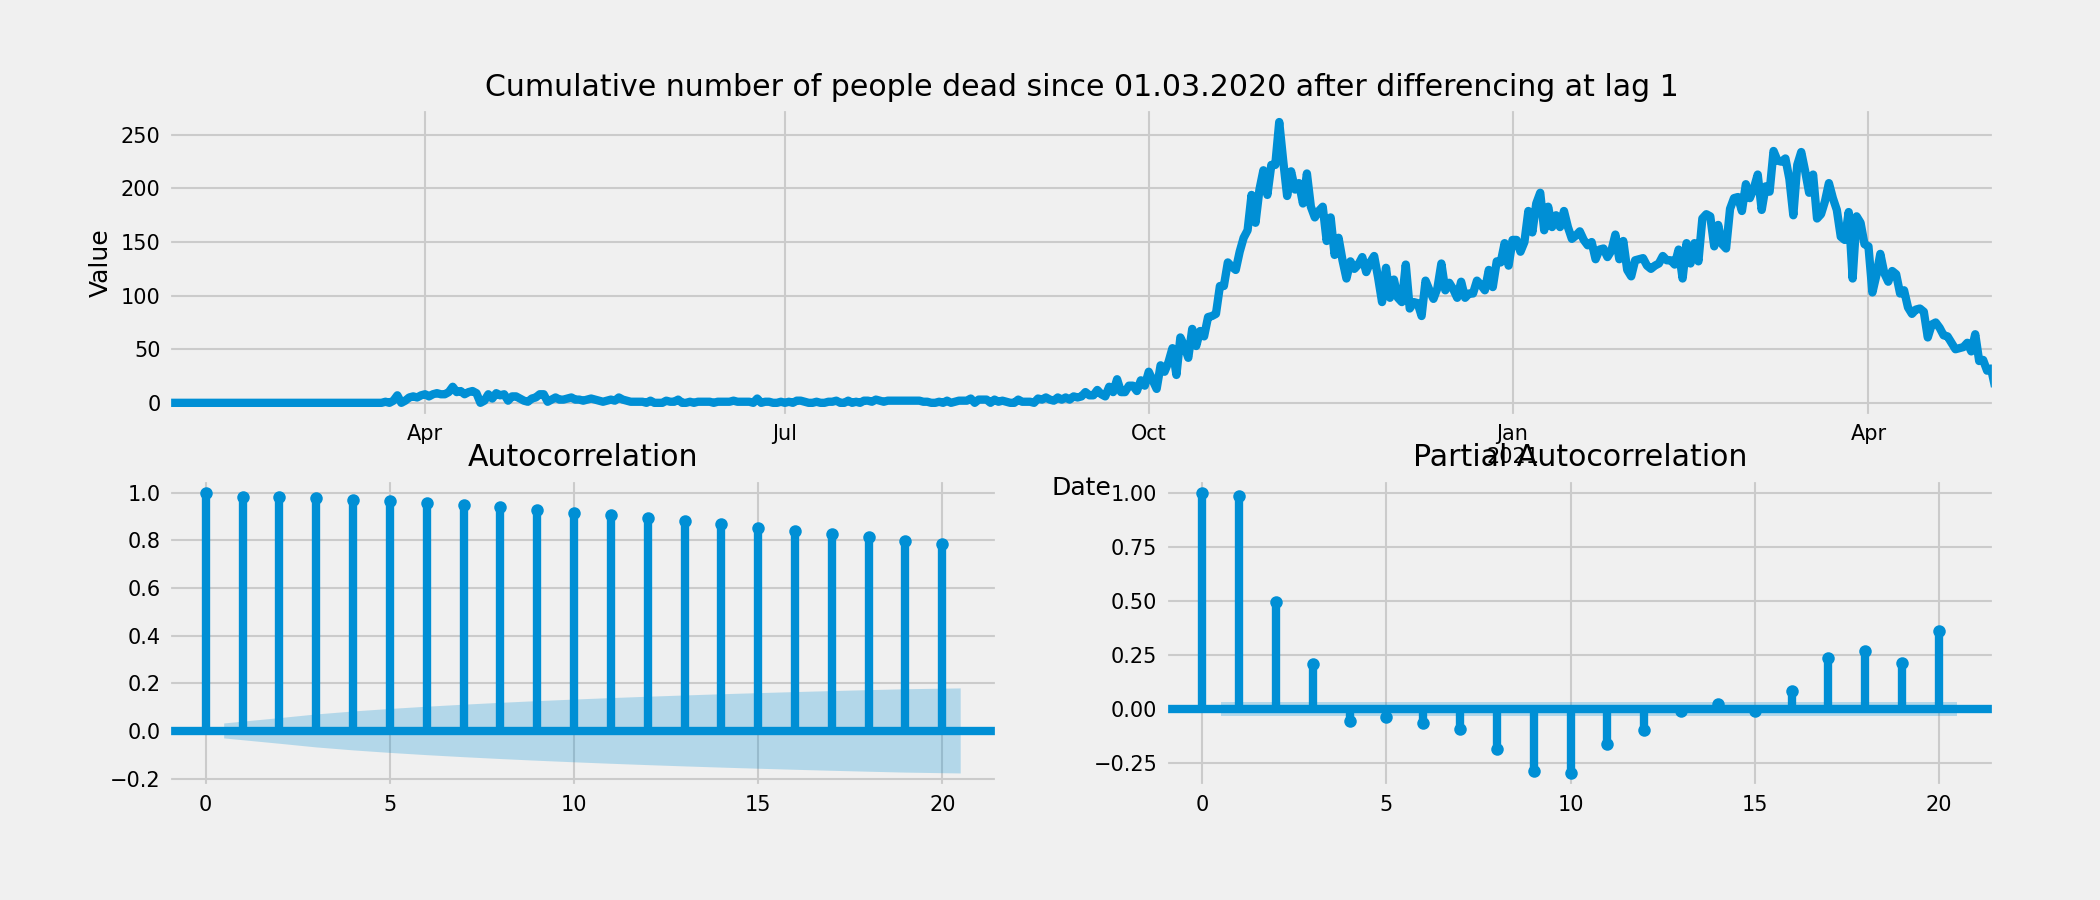
\includegraphics[width=1\textwidth, height=0.3\textwidth]{figures/chapter_04/dead_ts/ts_diff_dead.png}
  \label{fig:dead_diff}} \\
  \subfloat[c][The cumulative number of people dead time series after double differencing at lag 1.]{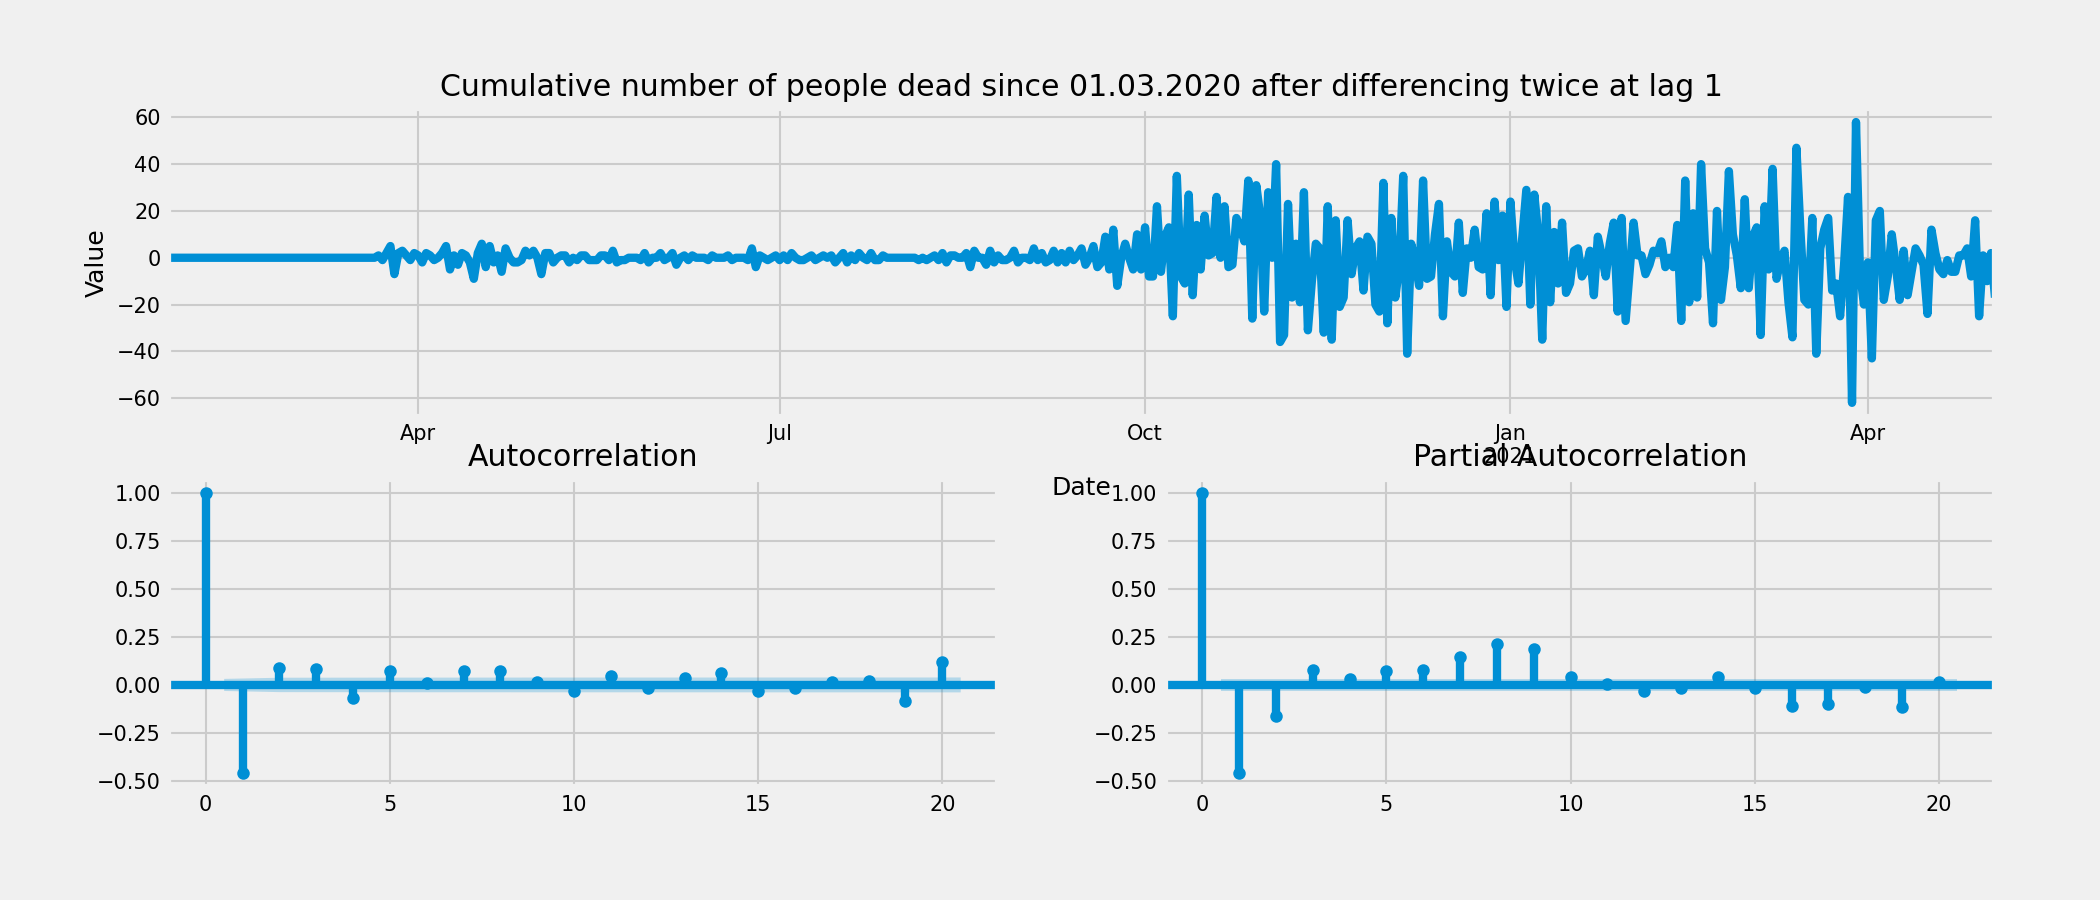
\includegraphics[width=1\textwidth, height=0.3\textwidth]{figures/chapter_04/dead_ts/ts_diff1_1_dead.png}
  \label{fig:dead_diff_1_1}} \\
  \caption{The cumulative amount of people cured after different differencing sequences with the corresponding ACF and PACF.}
  \label{fig:dead_diff_ex}
\end{figure}
It is possible to reduce the heteroscedasticity in the data by application of, for example, Box-Cox or logarithmic transformations (according to their properties) or by dropping all measurements until June 1, 2020.

Table \ref{tab:dead_tests_table} shows that after at least one of these manipulations, the tests indicate the stationarity of the time series.

Now we can say that the cumulative number of people dead time series potentially can be modeled using ARIMA(0, 2, 1) model.

\begin{figure}[!htb]
  \centering
  \subfloat[a][The number of active cases time series]{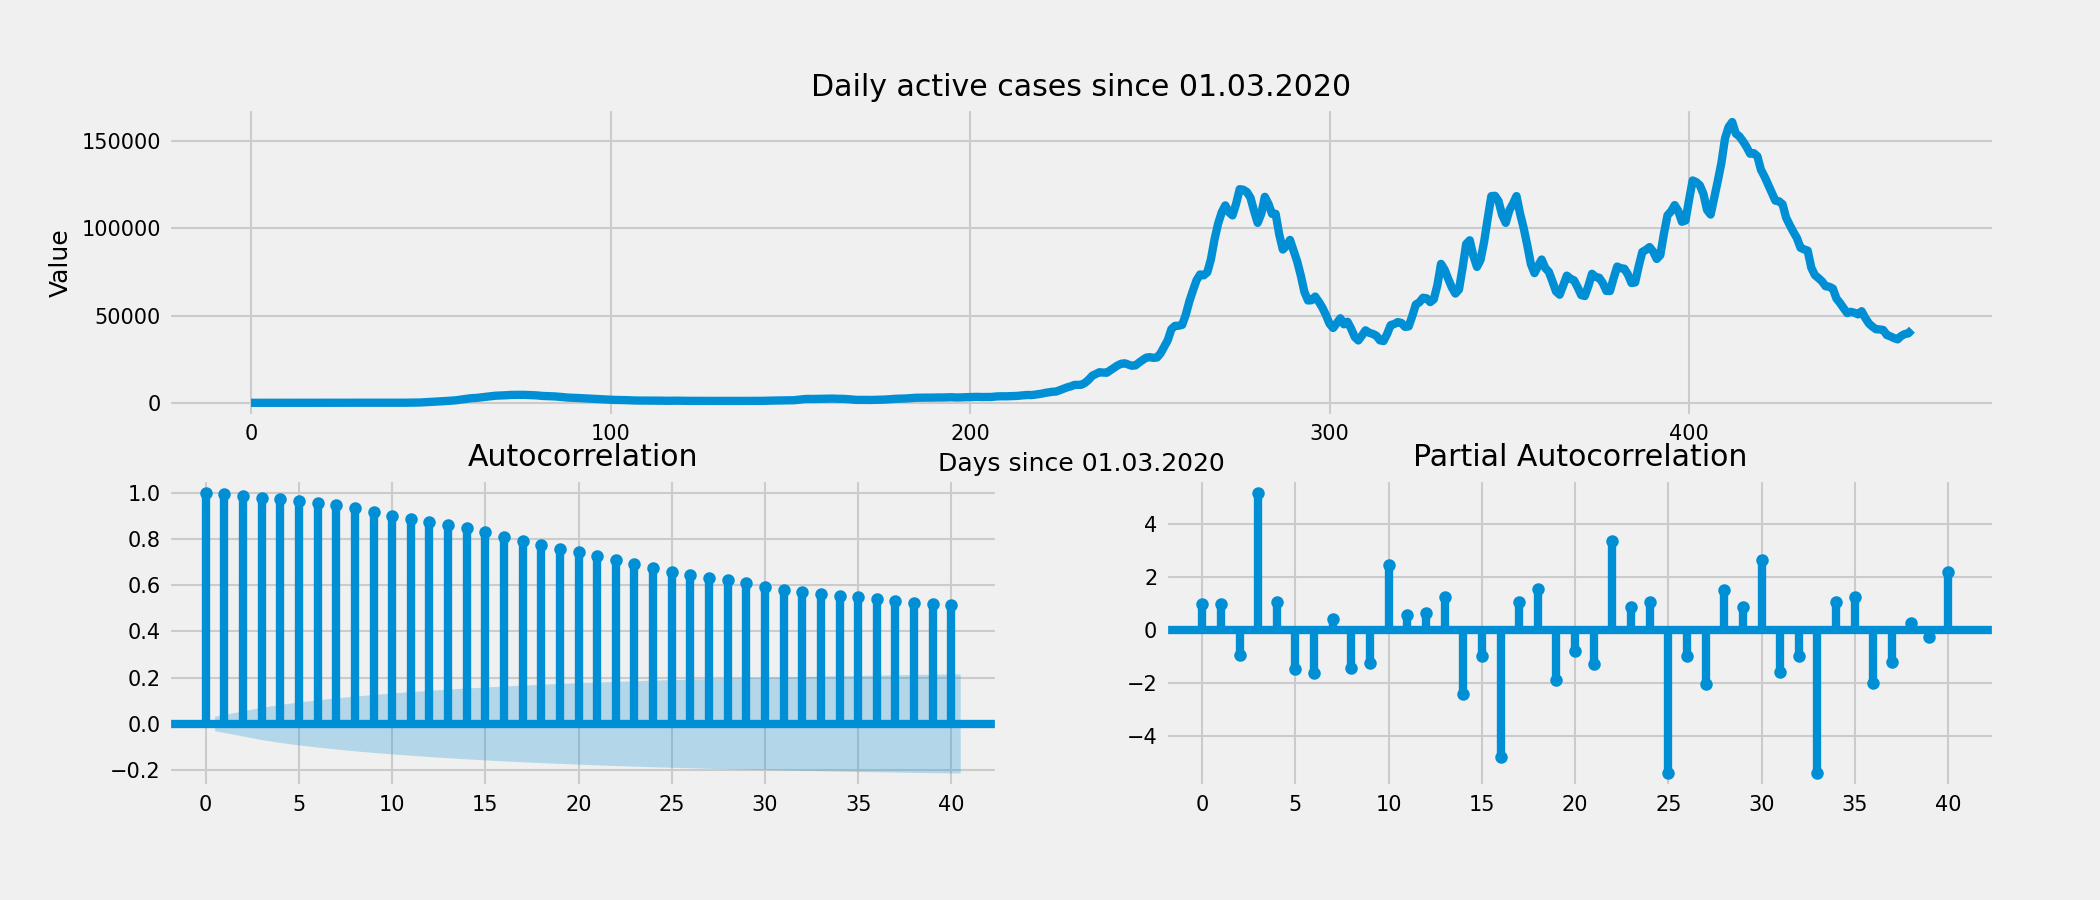
\includegraphics[width=1\textwidth, height=0.28\textwidth]{figures/chapter_04/original_ts/ts_orig_iactive.png}
  \label{fig:orig_active}} \\
  \subfloat[b][The number of active cases time series after differencing at lag 1.]{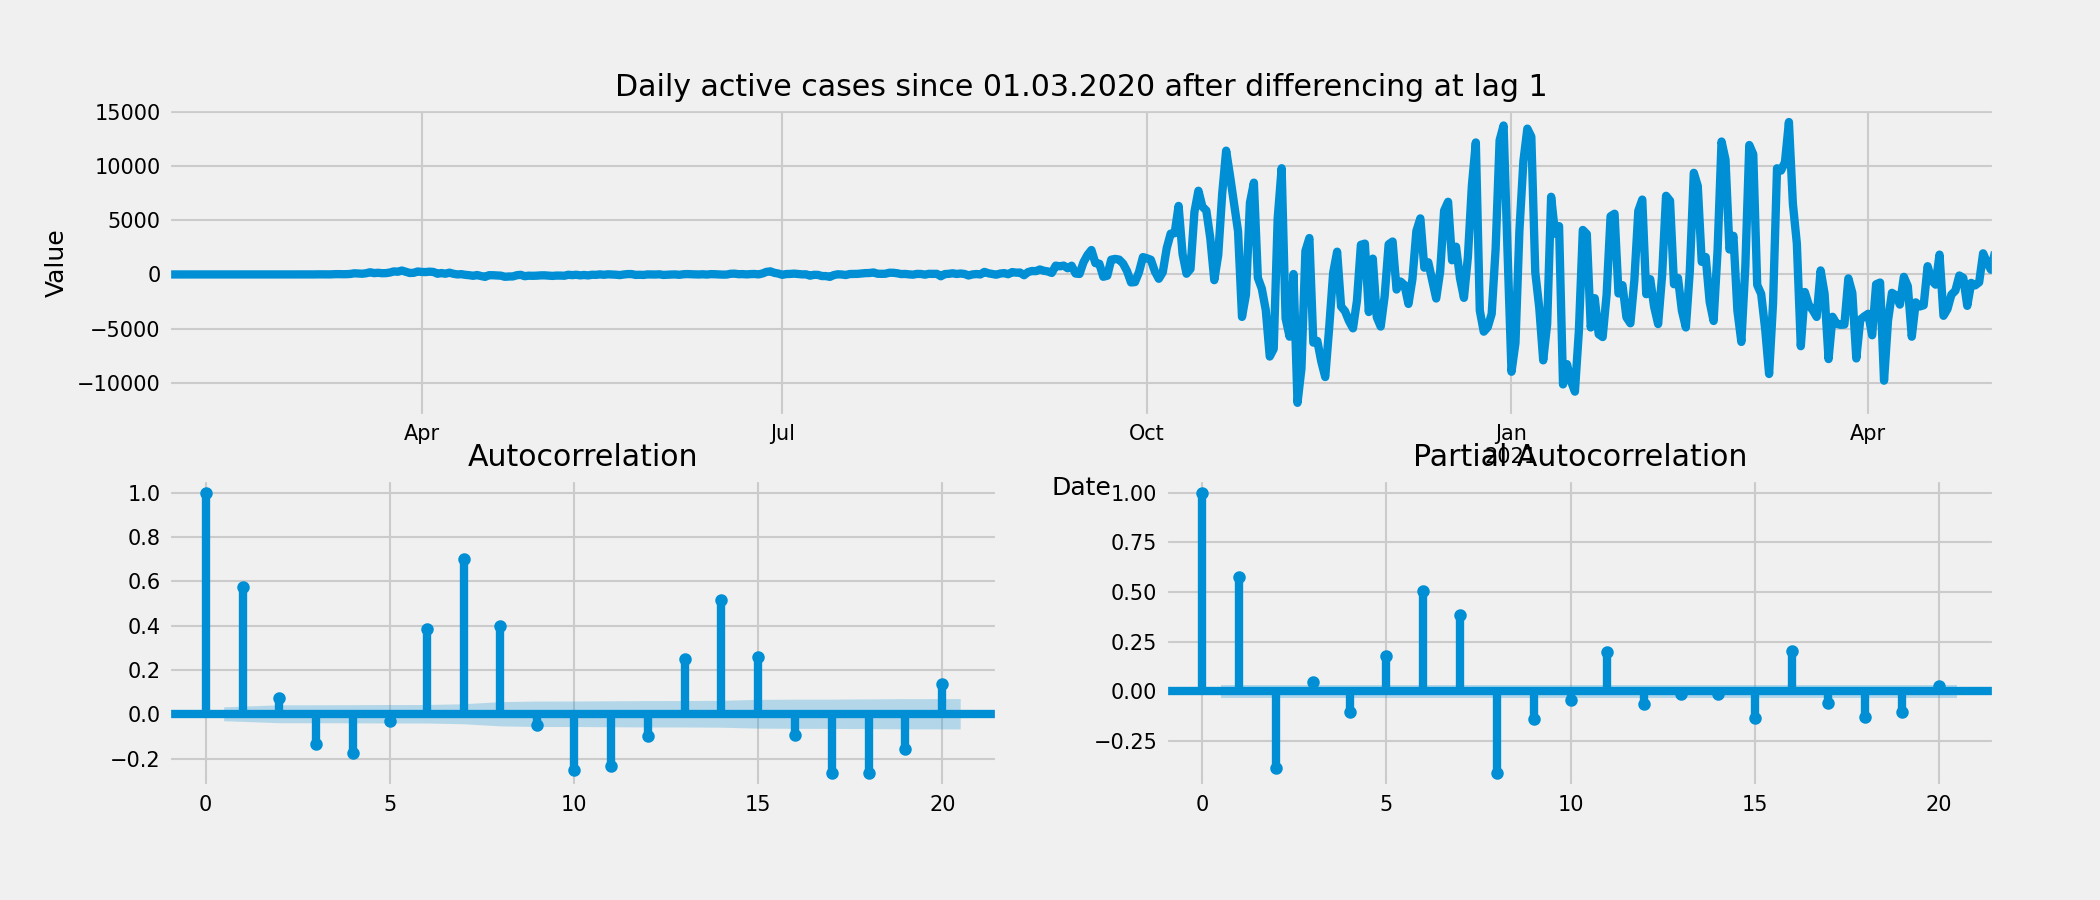
\includegraphics[width=1\textwidth, height=0.28\textwidth]{figures/chapter_04/active_ts/ts_diff_active.png}
  \label{fig:active_diff}} \\
  \subfloat[c][The number of active cases time series after differencing at lag 1 and lag 7.]{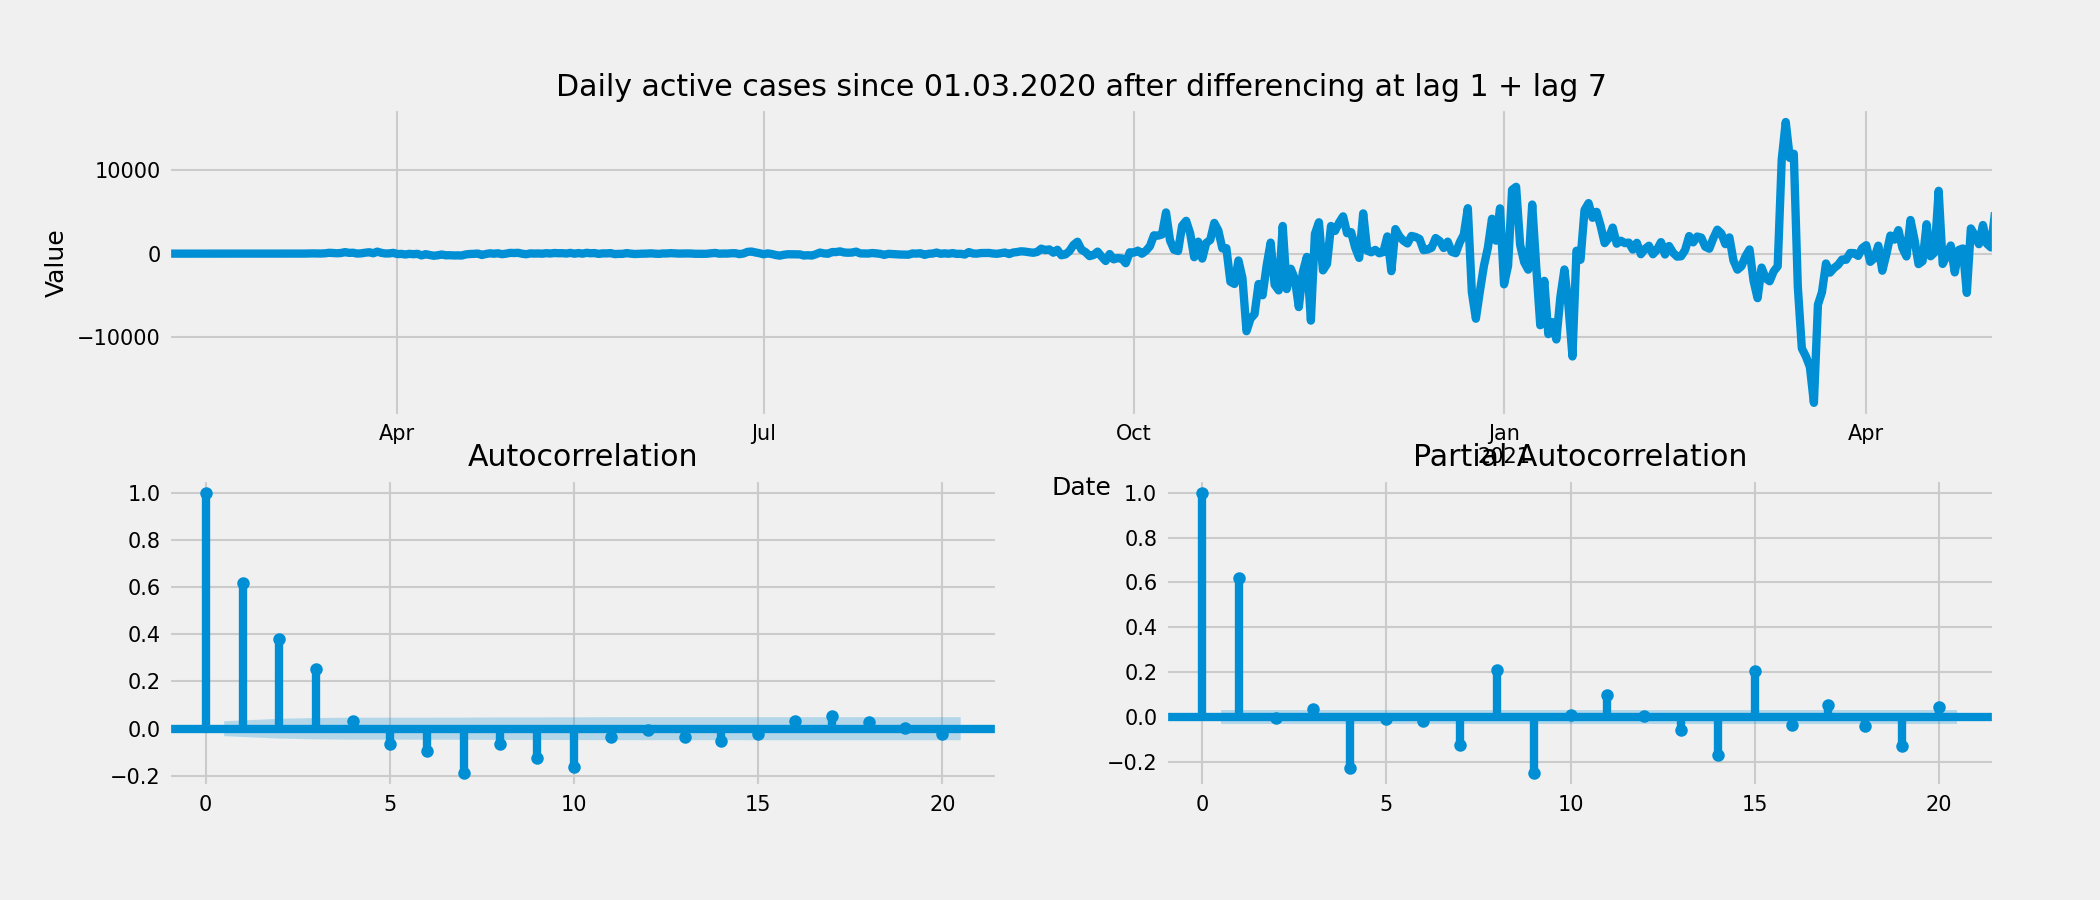
\includegraphics[width=1\textwidth, height=0.28\textwidth]{figures/chapter_04/active_ts/ts_diff1_7_active.png}
  \label{fig:active_diff_1_7}} \\
  \caption{The number of active cases time series after different differencing sequences with the corresponding ACF and PACF.}
  \label{fig:active_diff_ex}
\end{figure}

\subsection{The number of active cases time series}

The fourth selected time series describes the number of active cases. In Figure \ref{fig:orig_active} you can see it before any manipulation. It has a global trend, but we can say anything about the seasonal patterns or about the order of autoregressive and moving average components. Similar to the other time series, the period until June 1, 2020, is fundamentally different and does not contain any useful information. Stationarity testing (Table \ref{tab:active_tests_table}) indicates that the the time series is nonstationary. Thus, we need to perform differencing at lag 1.

Figure \ref{fig:active_diff} shows that after the first differencing we got rid of the global trend, plus it is now clear that there is a seasonal pattern with weekly periodicity. The ACF and PACF show that the order of the seasonal autoregressive component is equal to 1 (significant correlation at lags 7, 14, and so on). According to the tests, the time series is now stationary. However, it is difficult to determine the order of the general autoregressive or moving average component. 

After differencing at lag 7 (to remove seasonality), it is visible that the order of the general autoregressive component is equal to 1 (the value of the ACF slowly decreases, the value of the PACF drops after lag 1).

\begin{table}[!ht]
    \centering
    \begin{tabular}{|p{3cm}||p{3cm}| p{3cm}|}
    \hline
    Time series & Dikey-Fuller test p-value & KPSS test p-value\\
    \hline
    Original time series& 0.290402 & 0.017614\\
	\hline
	1x at lag 1 & 0.000158 & 0.100000\\
	\hline
	1x at lag 1; 1x at lag 7 &  0.000005 & 0.100000\\
	\hline
\end{tabular}
    \caption{The number of active cases: results of the stationarity tests.}
    \label{tab:active_tests_table}
\end{table}

To summarize, this time series can be modeled using the SARIMA(1, 1, 0) $\times$ (1, 0, 0$)_7$ or SARIMA(1, 1, 0) $\times$ (1, 1, 0$)_7$ models.

\hypertarget{s3.3}{\section{Facebook Prophet modeling}}

After applying the basic analysis, the selected time series are ready for modeling using the Facebook Prophet model. 

In this section, the more detailed pipeline has been formulated as
\begin{enumerate}
    \item find the best configuration of all 3 defined components (trend, seasonal, holidays) for each selected time series.
    \item perform hyperparameters tuning using the cross-validation.
    \item evaluate the model using specified metrics.
    \item obtain a set of changepoints for each time series individually, evaluate the possibility of using a single shared set for all selected time series.
    \item create a custom set of changepoints based on the public information about restrictions provided by the Czech government and compare it with automatically detected
    \item perform the forecasts
    \item find some correlations between government restrictions and changes in the growth rate of the selected time series.
\end{enumerate}

As we found out in the section of time series analysis, all selected time series have a part significantly distinct from the remaining time series (for example, until June 1, 2020), where nothing special happens. We can ignore this data during the future modeling (because this period has no information about the evolution of the COVID-19 pandemic since the first wave). However, the Facebook Prophet model supports the global trend growth changes, so it will be enough to drop the period with the target variable equal to 0.

\subsection{Parameter estimation mechanism}

According to the specified pipeline, the first step is to perform hyperparameter tuning using the time series cross-validation technique. 

We need to define the parameters of the cross-validation. It is also necessary to specify the parameters of the model used during the cross-validation that will can set manually. We will use the knowledge received during the basic time series analysis and the information from the official Facebook Prophet documentation \cite{ProphetDoc}.

The cross-validation parameters are: 
\begin{itemize}
    \item initial cutoff $=$ 150 days ($\sim$ July 1, 2020, covers the beginning of the useful data),
    \item forecast horizon $=$ 14 days (this value was selected because it is equal to 2 $\times$ length of the seasonal pattern and can be potentially useful during the pandemic analysis).
\end{itemize}

The manually specified parameters of the model are \textit{set of holidays} and \textit{seasonality} (for seasonal time series).

The set of holidays is specified using the inbuilt method of the Prophet model that adds a list of national holidays (depends on the country).

Table \ref{tab:holidays_set} demonstrates the curtain list of holidays specified for the Czech Republic.

\begin{table}[!ht]
    \centering
    \begin{tabular}{|p{1cm}||p{8cm}|}
    \hline
    Index & Holiday name\\
    \hline
    0 & Day of the Restoration of the Independent Czech State \\
    \hline
    1 & Good Friday\\
    \hline
    2 & Easter Monday\\
    \hline
    3 & Labor Day\\
    \hline
    4 & Victory Day\\
    \hline
    5 & Day of the Slavic heralds Cyril and Methodius\\
    \hline
    6 & Day of the burning of master Jan Hus\\
    \hline
    7 & Czech Statehood Day\\
    \hline
    8 & Day of the establishment of an independent Czechoslovak state\\
    \hline
    9 & Day of the Struggle for Freedom and Democracy\\
    \hline
    10 & Christmas Eve\\
    \hline
    11 & 1st Christmas holiday\\
    \hline
    12 & 2nd Christmas holiday\\
    \hline
\end{tabular}
    \caption{The set of holidays used in the Prophet modeling.}
    \label{tab:holidays_set}
\end{table}

For time series that contain seasonal patterns, we will also enable a \textit{weekly seasonality}. 

During the cross-validation, there is no need to compute the confidential intervals because we care only about the forecast accuracy in comparison with the historical data. 

We also will cut the last 14 days off to evaluate model performance on the unseen data.

\subsubsection{Data transformation before modeling}

For the Prophet modeling, we decided to drop the first 55 days (until the day of the first death) to get rid of measures with zero value and remain equal length of the selected time series.

\subsubsection{Cross-validation accuracy metrics}

For evaluation of the cross-validation results, we decided to use MAPE metric supported by the cross-validation function inside the Prophet diagnostics module \cite{ProphetDoc}: 
\begin{equation}
    MAPE = \frac{100}{n}\sum_{t=1}^{n}\Big|\frac{Y_t - \hat{Y_t}}{Y_t}\Big|,
\end{equation}    
where $n$ is an amount of forecasted points, $Y_t$ is the real value of the observed variable $Y$ at timestamp $t$, and $\hat{Y_t}$ is the forecasted value at timestamp $t$.

As we noticed earlier in Chapter \hyperlink{ch3}{3}, the resulting error is computed as the mean of the errors obtained from all forecasts made during the cross-validation process.  

According to the fact that we have selected 4 different time series, we will perform 4 different cross-validations.

Table \ref{tab:cross_val_grid} contains information about the parameters to tune.

\begin{table}[!ht]
    \centering
    \begin{tabular}{|p{6cm}||p{4cm}|}
    \hline
    Parameter name & Possible values\\
    \hline
    \verb|changepoint_prior_scale| & 0.1, 0.5, 0.8, 1.0\\
    \hline
    \verb|seasonality_prior_scale| & 0.1, 1.0, 10.0\\
    \hline
    \verb|seasonality_mode| & multiplicative, additive\\
    \hline
    \verb|holidays_prior_scale| & 0.1, 1.0, 10.0\\
    \hline
    \verb|changepoint_range| & 0.8, 0.9, 0.95\\
    \hline
\end{tabular}
    \caption{The Prophet cross-validation parameter grid.}
    \label{tab:cross_val_grid}
\end{table}

The \verb|changepoint_prior_scale| parameter corresponds to the parameter $\tau$ of the Laplace distribution (Section \ref{sec:automatic_cp_detection}). It controls the growth rate change flexibility. The \verb|seasonality_prior_scale| parameter (for seasonal time series )regulates strength of the seasonal model. According to the official Prophet documentation \cite{ProphetDoc}, larger values allow larger seasonal fluctuations, smaller values mitigate the seasonality. The \verb|seasonality_mode| parameter specifies a type of seasonal model (multiplier or addendum). The \verb|holidays_prior_scale| parameter controls the sensitivity to the changes caused by holidays. The \verb|changepoint_range| parameter defines the percentage of the time series (from the beginning) within which the changepoints will be distributed.

\subsubsection{Cross-validation results}

Table \ref{tab:cross_val_res} contains information about the best performance parameters for each model.

\begin{table}[!ht]
\catcode`\-=12
\centering
\resizebox{\textwidth}{!}{%
\begin{tabular}{|l|l|l|l|}
\hline
 &
  \multicolumn{2}{l|}{\textit{\textbf{Parameter}}} &
  \textit{\textbf{Error}} \\ \hline
\textbf{Time series} &
  \textbf{Name} &
  \textbf{Value} &
  \textbf{MAPE (\%)} \\ \hline
\multirow{5}{*}{\begin{tabular}[c]{@{}l@{}}Cumulative number \\ of people infected\end{tabular}} &
  changepoint\_prior\_scale &
  0.8 &
  \multirow{5}{*}{5.314} \\ \cline{2-3}
 & seasonality\_prior\_scale & 10.0  &  \\ \cline{2-3}
 & seasonality\_mode         & 10.0 &  \\ \cline{2-3}
 & holidays\_prior\_scale    & additive &  \\ \cline{2-3}
 & changepoint\_range        & 0.95 &  \\ \hline
\multirow{5}{*}{\begin{tabular}[c]{@{}l@{}}Cumulative number \\ of people cured\end{tabular}} &
  changepoint\_prior\_scale &
  1.0 &
  \multirow{5}{*}{5.381} \\ \cline{2-3}
 & seasonality\_prior\_scale & 1.0 &  \\ \cline{2-3}
 & seasonality\_mode         & additive &  \\ \cline{2-3}
 & holidays\_prior\_scale    & 10.0 &  \\ \cline{2-3}
 & changepoint\_range        & 0.95  &  \\ \hline
\multirow{3}{*}{\begin{tabular}[c]{@{}l@{}}Cumulative number \\ of people dead\end{tabular}} &
  changepoint\_prior\_scale &
  1.0 &
  \multirow{3}{*}{5.111} \\ \cline{2-3}
 & holidays\_prior\_scale    & 1.0  &  \\ \cline{2-3}
 & changepoint\_range        & 0.95 &  \\ \hline
\multirow{5}{*}{\begin{tabular}[c]{@{}l@{}}Number of active \\ cases\end{tabular}} &
  changepoint\_prior\_scale &
  1.0 &
  \multirow{5}{*}{28.957} \\ \cline{2-3}
 & seasonality\_prior\_scale & 10.0  &  \\ \cline{2-3}
 & seasonality\_mode         & mult. &  \\ \cline{2-3}
 & holidays\_prior\_scale    & 0.1 &  \\ \cline{2-3}
 & changepoint\_range        & 0.95 &  \\ \hline
\end{tabular}%
}
\caption{The best set of the hyperparameters for each time series.}
\label{tab:cross_val_res}
\end{table}

It is visible that the cross-validation results are relatively satisfactory. Average MAPE varies between 5-28\%. 

The number of active cases time series has a larger average MAPE because it has more expressive growth changes (other time series contain a cumulative sum, this time series contains information about daily active cases). It means that, on average, the data before and after cutoffs have more distinct differences in trend directions. It can potentially affect the future forecast of the unseen data. To reduce this problem, we decided to apply \textit{the log transformation} on this time series (according to the fact that we need to apply an inverse transform to all forecast components, we cant use Box-Cox transformation\footnote{https://github.com/facebook/prophet/issues/647 ---  Box-Cox transformation usage with Prophet problem, the inverted sum does not equal to the sum of inverted components}). 

Logarithm transformation can invert the sum in such a way that it will be equal to the product of inverted components (additive model to multiplicative, because of the logarithm). Table \ref{tab:cross_val_act_log} shows cross-validation results after this transformation. We have reduced the average MAPE from 28\% to 2.5\%. 

\begin{table}[!htb]
\catcode`\-=12
\centering
\resizebox{\textwidth}{!}{%
\begin{tabular}{|l|l|l|l|}
\hline
 &
  \multicolumn{2}{l|}{\textit{\textbf{Parameter}}} &
  \textit{\textbf{Error}} \\ \hline
\textbf{Time series} &
  \textbf{Name} &
  \textbf{Value} &
  \textbf{MAPE (\%)} \\ \hline
\multirow{5}{*}{\begin{tabular}[c]{@{}l@{}}Number of active \\ cases + log. \\ transformation\end{tabular}} &
  changepoint\_prior\_scale &
  1.0 &
  \multirow{5}{*}{2.455} \\ \cline{2-3}
 & seasonality\_prior\_scale & 10.0  &  \\ \cline{2-3}
 & holidays\_prior\_scale    & 10.0 &  \\ \cline{2-3}
 & seasonality\_mode         & additive &  \\ \cline{2-3}
 & changepoint\_range        & 0.95 &  \\ \hline
\end{tabular}%
}
\caption{The best set of the hyperparameters for the number of active cases time series after the logarithm transformation.}
\label{tab:cross_val_act_log}
\end{table}

\begin{figure}[!htb]
  \centering
  \subfloat[a][Modeled time series.]{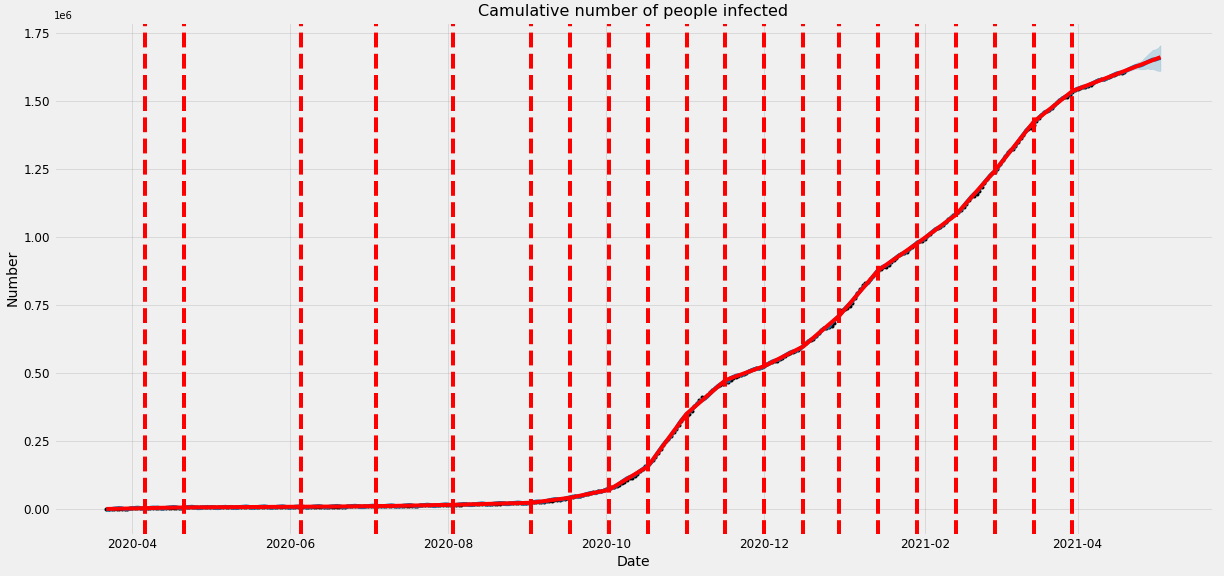
\includegraphics[width=1\textwidth, height=0.4\textwidth]{figures/chapter_04/forecast_example/infected_fbp_modeled.png}
  \label{fig:infected_modeled}} \\
  \subfloat[b][Forecast components.]{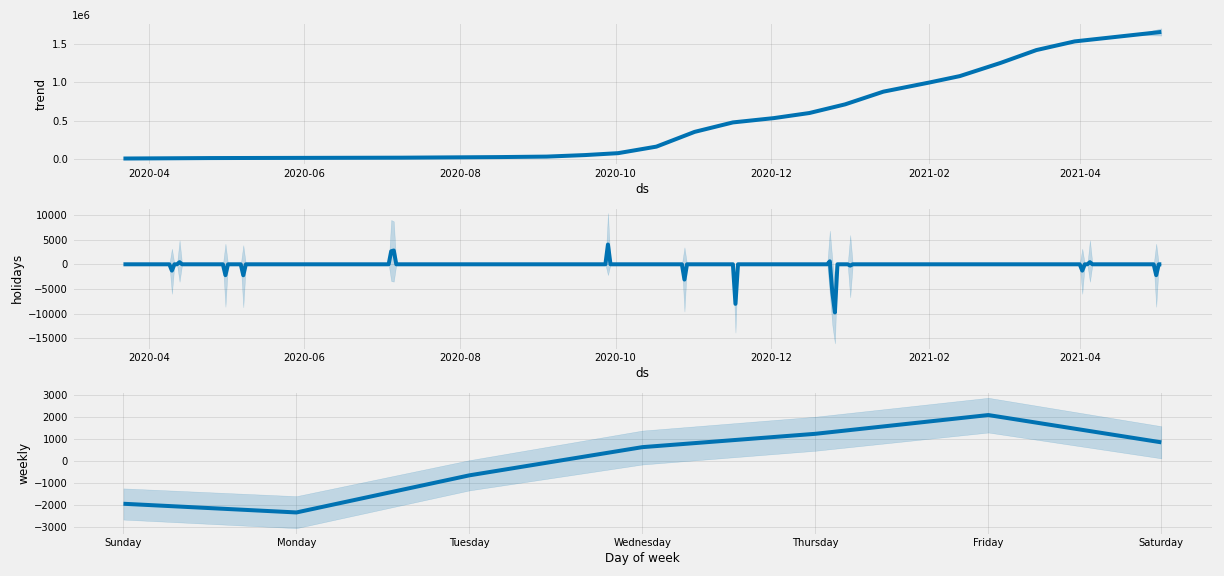
\includegraphics[width=1\textwidth, height=0.4\textwidth]{figures/chapter_04/forecast_example/infected_fbp_components.png}
  \label{fig:infected_modeled_components}} \\
  \caption{The cumulative amount of people infected modeled using the Prophet model + Forecast components.}
  \label{fig:infected_forecast_fbp}
\end{figure}

Now, we can fit new models (using tuned parameters) for each time series to analyze changepoints distribution and forecast accuracy for unseen data (the last 14 days of observations).
\hypertarget{ss332}{\subsection{Forecasting using Prophet model}}

After fitting new models to the data, it is possible to perform a forecast with 14 days forecast horizon. Figure \ref{fig:infected_forecast_fbp} shows an example of the resulting model plot with extra information about each forecast component individually. Additionally, in Figure \ref{fig:infected_forecast_last} you can see a more detailed graph with the comparison of the forecasted and the original data since the last detected changepoint (May 30, 2021) for each selected time series.

\begin{figure}[!ht]
\centering
\subfloat[a][Cumulative number of people infected time series forecast]{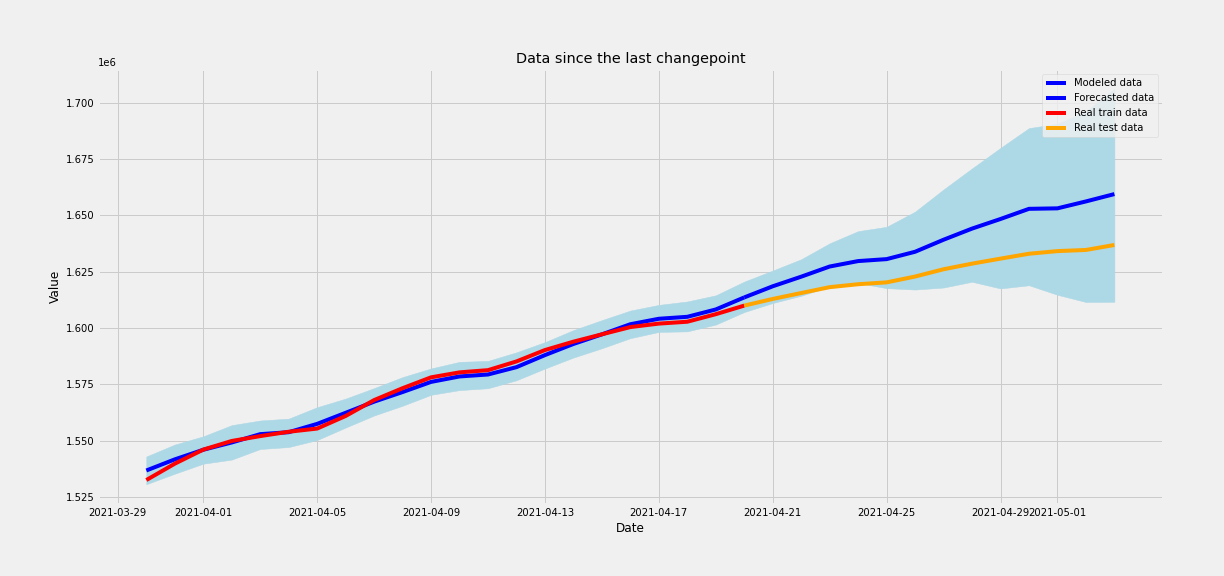
\includegraphics[width=1\textwidth, height=0.28\textwidth]{figures/chapter_04/forecast_example/forecast_infected_fc.png}\label{fig:infected_forecast_last}} \\
\subfloat[b][Cumulative number of people cured time series forecast]{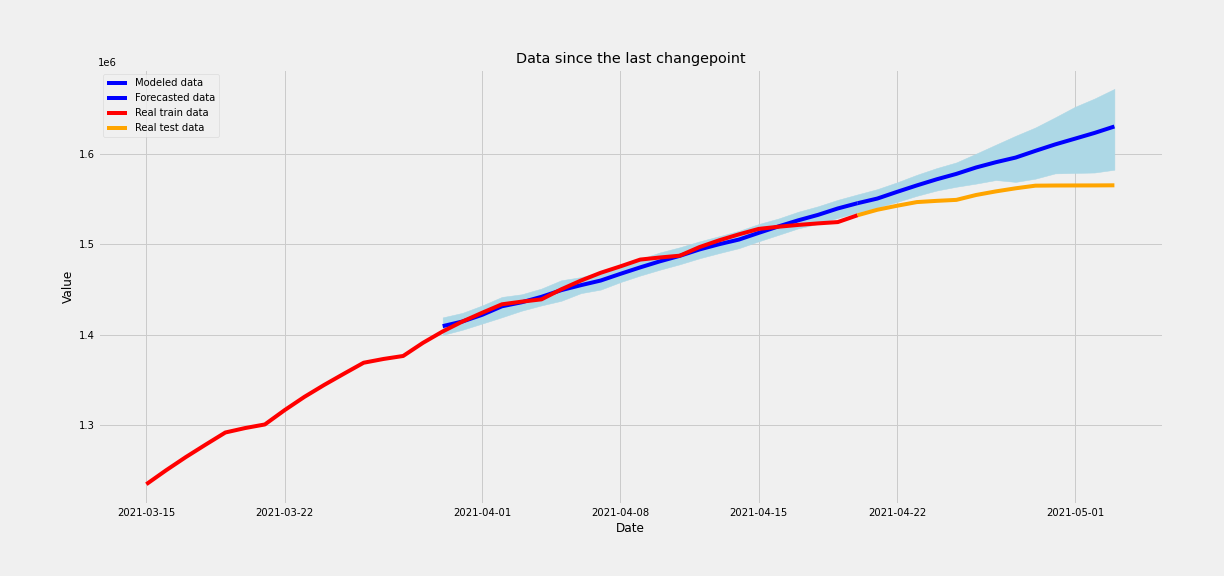
\includegraphics[width=1\textwidth, height=0.28\textwidth]{figures/chapter_04/forecast_example/forecast_cured_fc.png}\label{fig:cured_forecast_last}} \\
\subfloat[c][Cumulative number of people dead time series forecast]{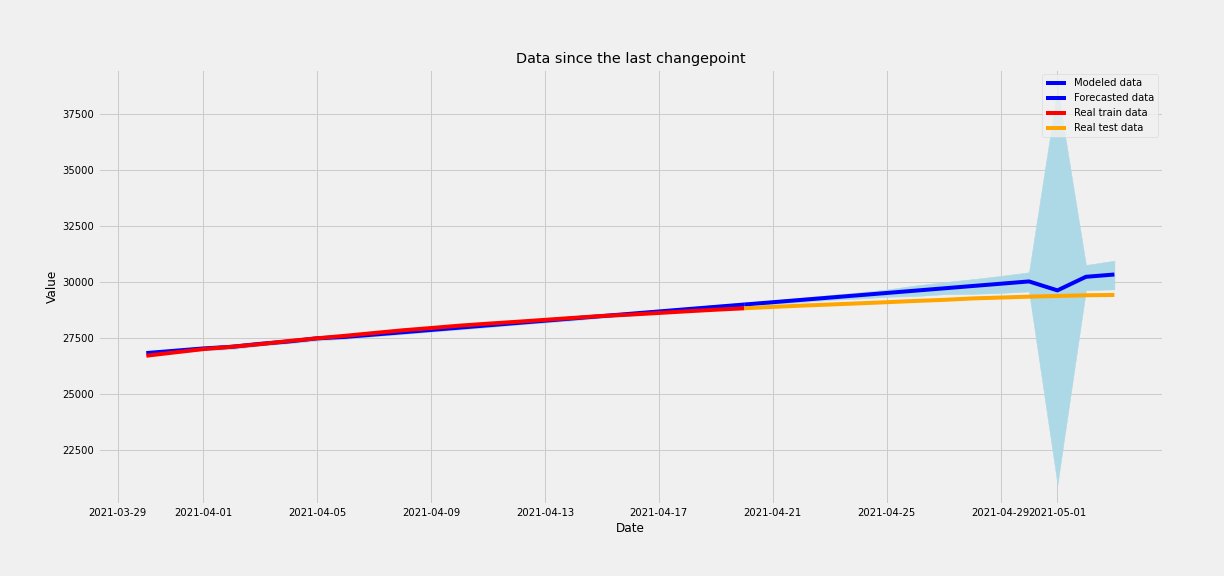
\includegraphics[width=1\textwidth, height=0.28\textwidth]{figures/chapter_04/forecast_example/forecast_dead_fc.png}\label{fig:dead_forecast_last}} \\
\subfloat[d][Number of active cases time series forecast]{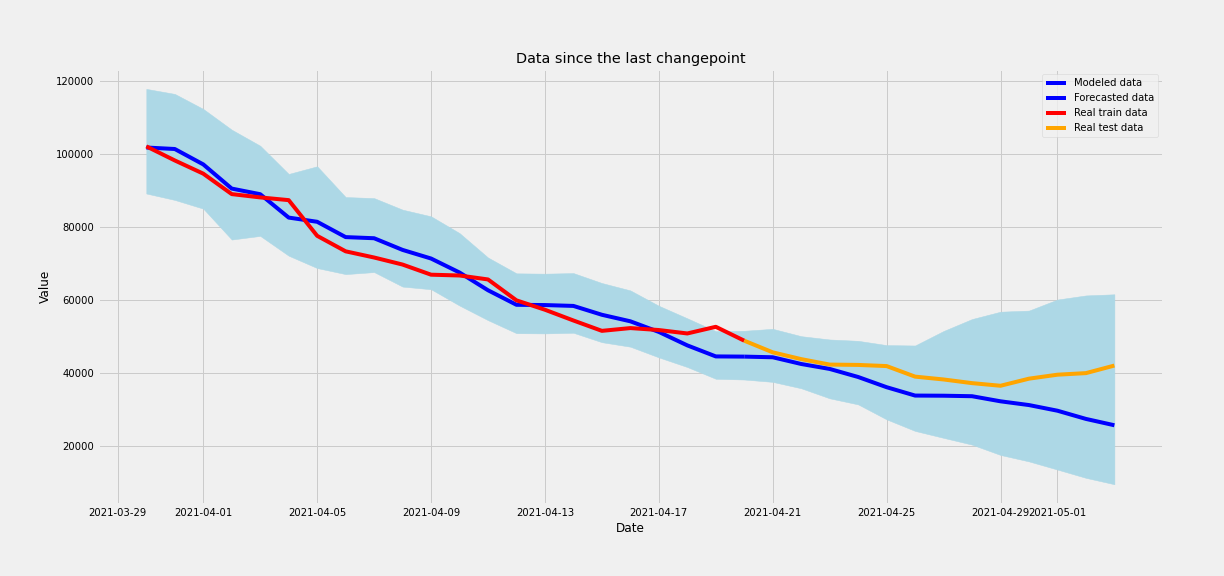
\includegraphics[width=1\textwidth, height=0.28\textwidth]{figures/chapter_04/forecast_example/forecast_active_fc.png}\label{fig:active_forecast_last}} \\
\caption{The selected time series forecasts (since the last detected changepoint May 30, 2021).}
\label{fig:forecast_last}
\end{figure}

In case of the number of active cases time series, we also applied an inverse transformation to compare the forecast with the original data.

According to the graph above, the confidence intervals become dramatically wide after the first forested week. In case of the number of people dead, there is no enough data to include the influence of the Labor day (May 1, 2021), which follows extremely wide confidence intervals. This leads to the fact that only the first several forecasted days may be useful in practice.

In addition to the above visualizations, Table \ref{tab:forecast_results_1} contains information about forecast errors (MAPE). 

\begin{table}[!ht]
\centering
\begin{tabular}{|l|l|}
\hline
Time series                                                                     & Forecast MAPE (\%)\\ \hline
\begin{tabular}[c]{@{}l@{}}Cumulative number \\ of people infected\end{tabular} &  0.818 \\ \hline
\begin{tabular}[c]{@{}l@{}}Cumulative number\\ of people cured\end{tabular}     &     2.143         \\ \hline
\begin{tabular}[c]{@{}l@{}}Cumulative number\\ of people dead\end{tabular}      &      1.597         \\ \hline
\begin{tabular}[c]{@{}l@{}}Number of active\\ cases\end{tabular}                &      14.37         \\ \hline
\end{tabular}%
\caption{Results of the original time series forecast.}
\label{tab:forecast_results_1}
\end{table}

\hypertarget{ss333}{\subsection{Changepoints}}

\subsubsection{Automatically detected changepoints}

While models fitting during the previous subsection, we have obtained a list with the changepoints. It is important to say that the changepoint lists were almost identical for all 4 time series. It is possible, because: all 25 potential changepoints are normally distributed within the first 95\% of the time series (approx. twice a month). 

\begin{table}[!htb]
\centering
\begin{tabular}{|l|l|l|l|l|l||l|l|l|l|l|l|}
\hline
\multicolumn{2}{|l|}{Changepoint}& \multicolumn{4}{l||}{Time series} &\multicolumn{2}{l|}{Changepoint}& \multicolumn{4}{l|}{Time series} \\ \hline
№& Date & I     & C   & D   & A& № & Date & I     & C   & D   & A\\ \hline
1  & 2020-04-06 &    +    &    +    &   +     & + & 14 & 2020-10-17 &    +    &    +    &   +     & +      \\ \hline 
2  & 2020-04-21 &    +    &    +    &   +     & +  & 15 & 2020-11-01 &    +    &    +    &   +     & +      \\ \hline
3  & 2020-05-06 &    +    &    +    &   -     & +  & 16 & 2020-11-16 &    +    &    +    &   +     & +      \\ \hline
4  & 2020-05-21 &    +    &    -    &   +     & +  & 17 & 2020-12-01 &    +    &    +    &   +     & +      \\ \hline
5  & 2020-06-05 &    +    &    -    &   -     & +  & 18 & 2020-12-16 &    -    &    +    &   +     & +      \\ \hline
6  & 2020-06-20 &    +    &    -    &   -     & + &19 & 2020-12-30 &    +    &    +    &   +     & +      \\ \hline  
7  & 2020-07-04 &    +    &    +    &   -     & + &  20 & 2021-01-14 &    +    &    +    &   +     & +      \\ \hline
8  & 2020-07-19 &    -    &    -    &   +     & + & 21 & 2021-01-29 &    +    &    +    &   +     & +      \\ \hline 
9  & 2020-08-03 &    +    &    +    &   -     & + & 22 & 2021-02-13 &    +    &    +    &   +     & +      \\ \hline 
10  & 2020-08-18 &    +   &    -    &   -     & +  & 23 & 2021-02-28 &    +    &    -    &   +     & -      \\ \hline
11 & 2020-09-02 &    +    &    +    &   +     & + & 24 & 2021-03-15 &    +    &    +    &   +     & +      \\ \hline 
12 & 2020-09-17 &    +    &    +    &   +     & + & 25 & 2021-03-30 &    +    &    +    &   +     & +      \\ \hline 
13 & 2020-10-02 &    +    &    +    &   +     & + & - & - &   -   & - &  -  & - \\ \hline 
\end{tabular}
\caption{Automatically detected changepoints (date format: YYYY-MM-DD) including the information about their usage in different models.}
\label{tab:changepoints}
\end{table}
The model tries to find the best changepoints subset with the lowest sum of growth change rate coefficients. In the selected time series, the growth rate changes frequently. and almost all potential changepoints are included in the final subset.

Table \ref{tab:changepoints} contains information about the potential changepoints and their usage in all fitted models. 

It is visible that the final subsets are similar. However, not all potential changepoints were included in every model. 

In this thesis, we will use this changepoints to measure the influence of fitting the model to the slice of the historical data since some changepoints. Thus, we have fitted multiple models to different slices of each selected time series. In Table \ref{tab:slice_forecast} you can see the best forecast results for each time series.

\begin{table}[!hbt]
\centering
\begin{tabular}{|l|l|l|}
\hline
Time series                                                                     & Slice from & MAPE (\%)\\ \hline
\begin{tabular}[c]{@{}l@{}}Cumulative number \\ of people infected\end{tabular} &   2021-01-12 &   0.339   \\ \hline
\begin{tabular}[c]{@{}l@{}}Cumulative number \\ of people cured\end{tabular}    &    2020-12-30   &   0.291 \\ \hline
\begin{tabular}[c]{@{}l@{}}Cumulative number \\ of people dead\end{tabular}    &       2021-02-13     &  0.435     \\ \hline
\begin{tabular}[c]{@{}l@{}}Number of active\\ cases\end{tabular}                &     2020-09-17     &  7.993     \\ \hline
\end{tabular}
\caption{Best results obtained from model fit to the slice of original data (from the changepoint).}
\label{tab:slice_forecast}
\end{table}

As expected, the models that are fitted to the data slice, since some of the specified changepoints are more accurate, then the models that are fitted to all historical data. However, according to the following visualizations (Figure \ref{fig:forecast_last_b}), the confidence intervals are increasing even faster then before. 

It is important to admit that  we have disabled the holidays component, because it is not possible to compute their influence on the final forecast.

\begin{figure}[!ht]
\centering
\subfloat[a][Cumulative number of people infected time series forecast (fitted to the data since January 12, 2021)]{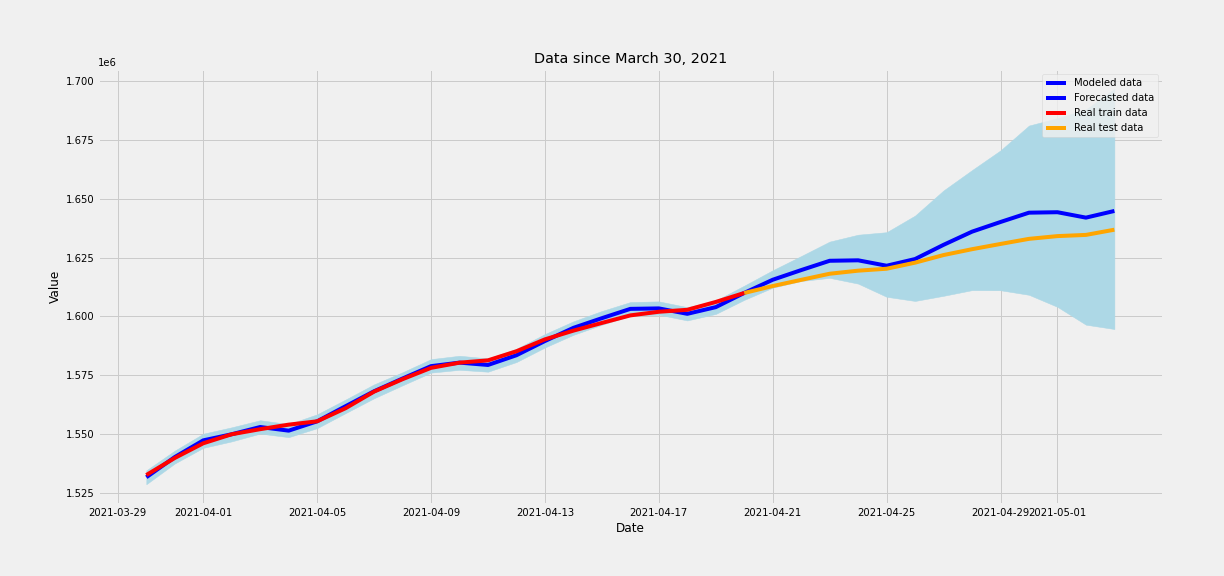
\includegraphics[width=1\textwidth, height=0.26\textwidth]{figures/chapter_04/forecast_example/forecast_infected_b_fc.png}\label{fig:infected_forecast_last_b}} \\
\subfloat[b][Cumulative number of people cured time series forecast (fitted to the data since December 30, 2020)]{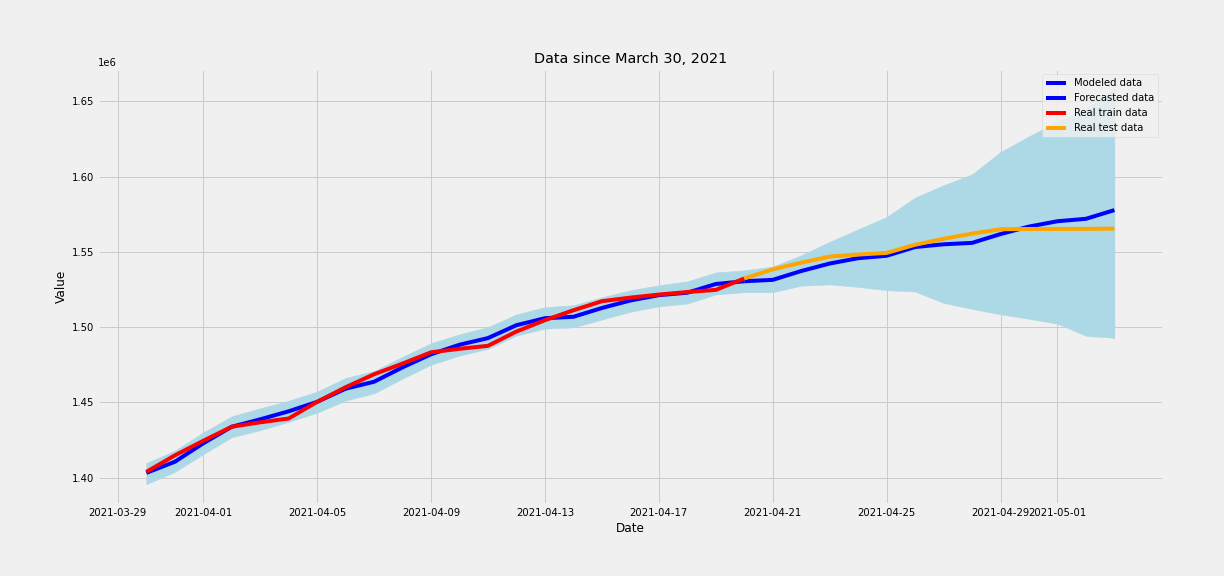
\includegraphics[width=1\textwidth, height=0.26\textwidth]{figures/chapter_04/forecast_example/forecast_cured_b_fc.png}\label{fig:cured_forecast_last_b}} \\
\subfloat[c][Cumulative number of people dead time series forecast (fitted to the data since February 13, 2021)]{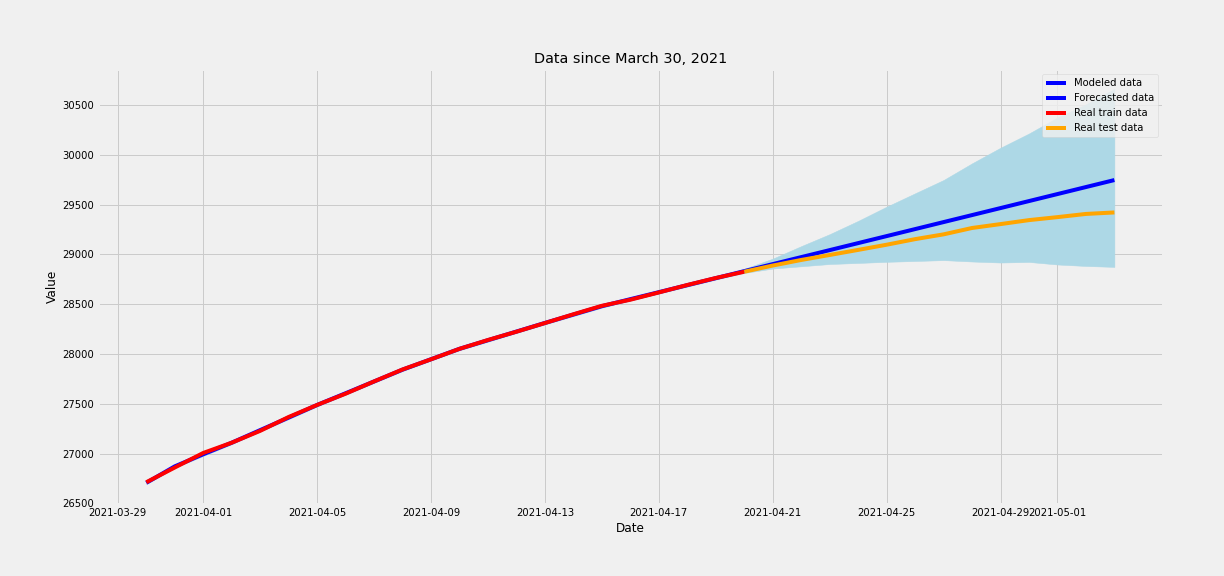
\includegraphics[width=1\textwidth, height=0.26\textwidth]{figures/chapter_04/forecast_example/forecast_dead_b_fc.png}\label{fig:dead_forecast_last_b}} \\
\subfloat[d][Number of active cases time series forecast (fitted to the data since September 17, 2020)]{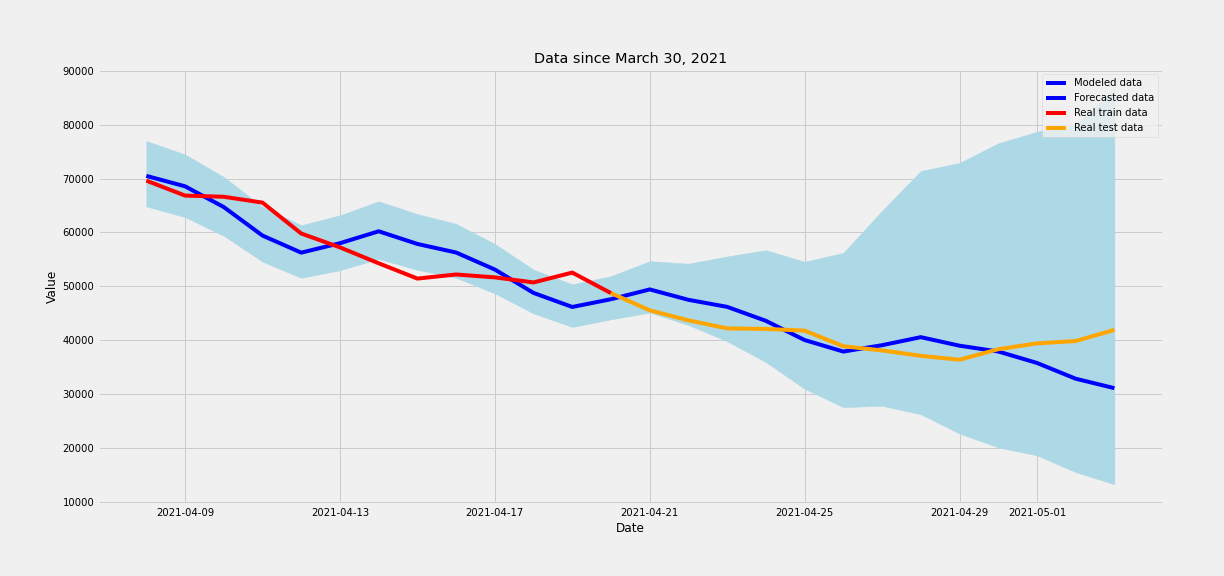
\includegraphics[width=1\textwidth, height=0.26\textwidth]{figures/chapter_04/forecast_example/forecast_active_b_fc.png}\label{fig:active_forecast_last_b}} \\
\caption{The selected time series forecasts (since March 30, 2021) fitted to the slice of data since the specified changepoint.}
\label{fig:forecast_last_b}
\end{figure}
\clearpage

\hypertarget{ss3.3.4}{\subsection{Interesting correlations between changepoints and government restrictions}}

One of the most interesting parts of this work is studying of the correlations between changepoints detected by the Prophet model (and their corresponding trend growth rate changes) and the list of government restrictions during the pandemic.

To perform this analysis, we have prepared the list of government restrictions since March 2, 2020. We have created our own list with 53 different restriction packs and other important events using the covid portal sponsored by the Ministry of the Interior of the Czech Republic \cite{covidportal}.

In this section, we will introduce some important and potentially useful correlations between changes in trend growth rate and some precursory measures before them.

\subsubsection{Correlation: Number of infected explosive growth slowdown}

The following figure shows a slice of the time series that contains measurements between October and January (year 2020). 

\begin{figure}[!ht]
\centering
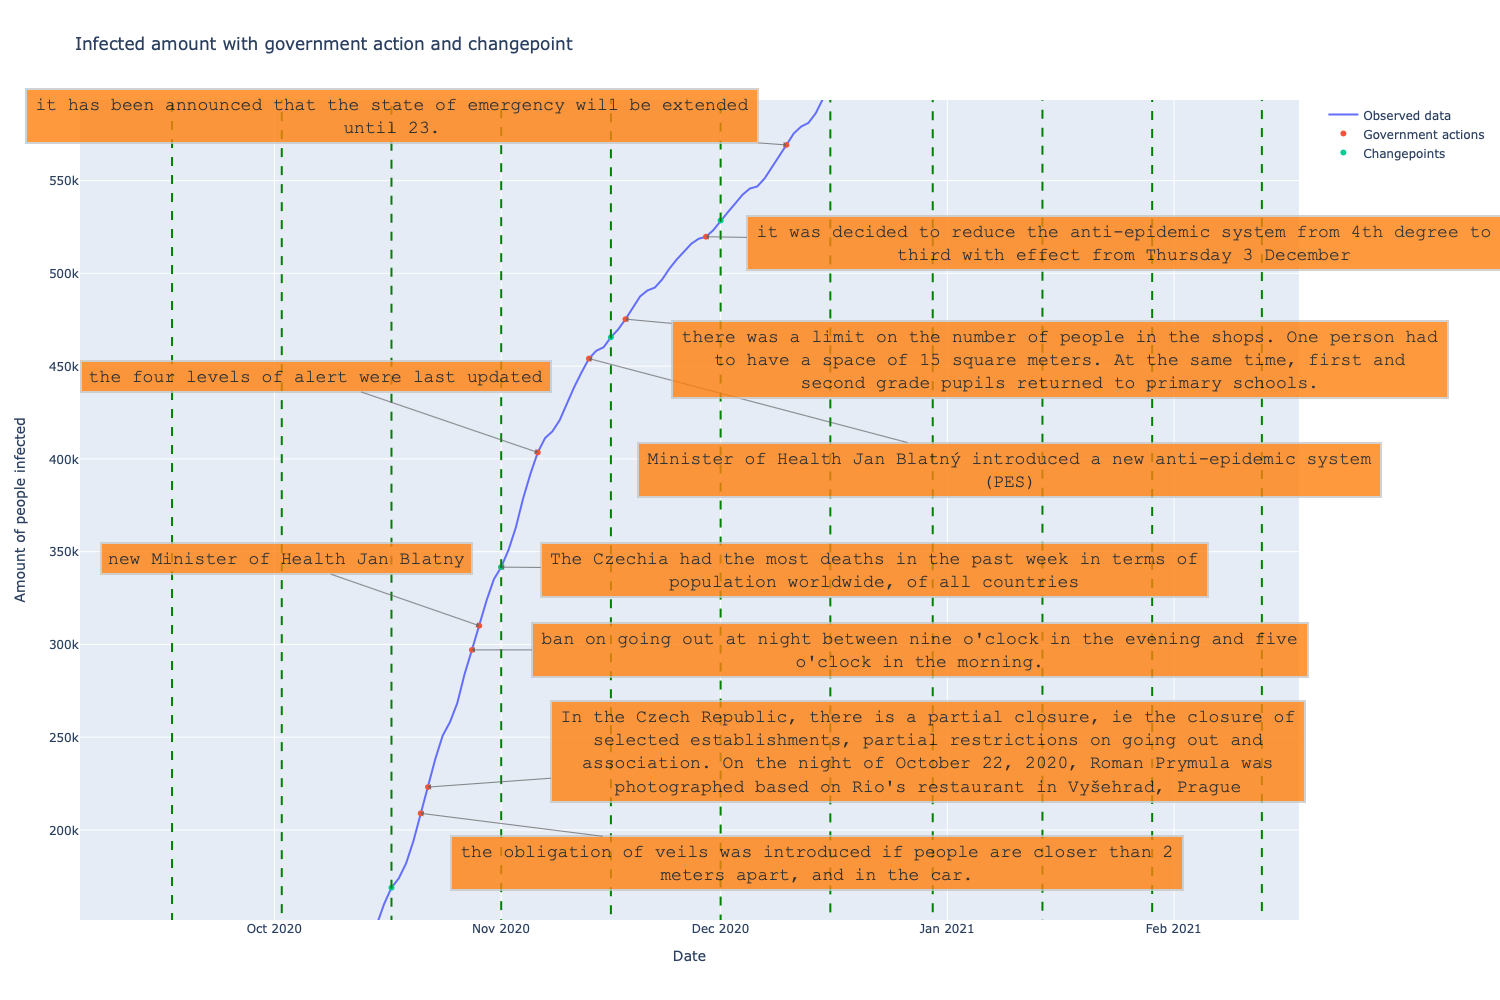
\includegraphics[width=1.0\textwidth, height=0.6\textwidth]{figures/chapter_04/changepoints_vs_government/infecred_expo_to_lin.png}
\caption{Cumulative number of infected growth slowdown October--November 2020.}
\label{fig:corr_inf_e_l}
\end{figure}

During this period, the increase in the number of cases has slowed from a sharply explosive to a calmer (potentially linear) but still rapid growth. The mean number of new cases between neighboring changepoints can be found in Table \ref{tab:new_cases_mean}. It decreased from 11665 to 4209.7 ($-227\%$).

\begin{table}[!htb]
\centering
\begin{tabular}{|l|l|l|}
\hline
Start date & End date & Mean number of active cases \\ \hline
2020-10-17 & 2020-11-01 &   11665.0  \\ \hline
2020-11-01 & 2020-11-16 &   8337.3  \\ \hline
2020-11-16 & 2020-12-01 &   4209.7  \\ \hline
\end{tabular}
\caption{Mean number of new cases daily between October 17, 2020 and December 1, 2020.}
\label{tab:new_cases_mean}
\end{table}

This change may indicate that the government restrictions occurred at a reasonable distance before they are potentially effective. In Figure \ref{fig:corr_inf_e_l} it is possible to see some labels that contain short descriptions of the restrictions between October 15, 2020, and December 15, 2020. \textbf{The most important are}: 
\begin{itemize}
    \item The obligation of face masks if people are closer than meters 2 apart (October 21, 2020).
    \item Partial closure (closure of selected establishments, October 22, 2020).
    \item Ban on going out at night between nine o'clock in the evening and five o'clock in the morning (October 28, 2020).
\end{itemize}

\subsubsection{Correlation: Number of infected explosive growth slowdown 2}

The second interesting slope change is depicted in Figure \ref{fig:corr_inf_e_l_2}. It occurs during the period between February 13, 2021 and May 3, 2021.

According to Table \ref{tab:new_cases_mean_2}, during February and the first half of March, the mean number of people infected daily had increased from 10169 to 11126. However, after March 15, it started to slow down to 3256 (on average) new cases daily ($-341\%$). 

\begin{table}[!htb]
\centering
\begin{tabular}{|l|l|l|}
\hline
Start date & End date & Mean number of active cases \\ \hline
2021-02-13 & 2021-02-28 & 10169.4 \\ \hline
2021-02-28 & 2021-03-15 & 11126.5 \\ \hline
2021-03-15 & 2021-03-30 & 8083.3 \\ \hline
2021-03-30 & 2020-05-03 & 3256.9 \\ \hline
\end{tabular}
\caption{Mean number of new cases daily between February 13, 2021 and May 3, 2021.}
\label{tab:new_cases_mean_2}
\end{table}

This slope change may indicate that potentially effective restrictions were in place prior to this period.

\begin{figure}[!htb]
\centering
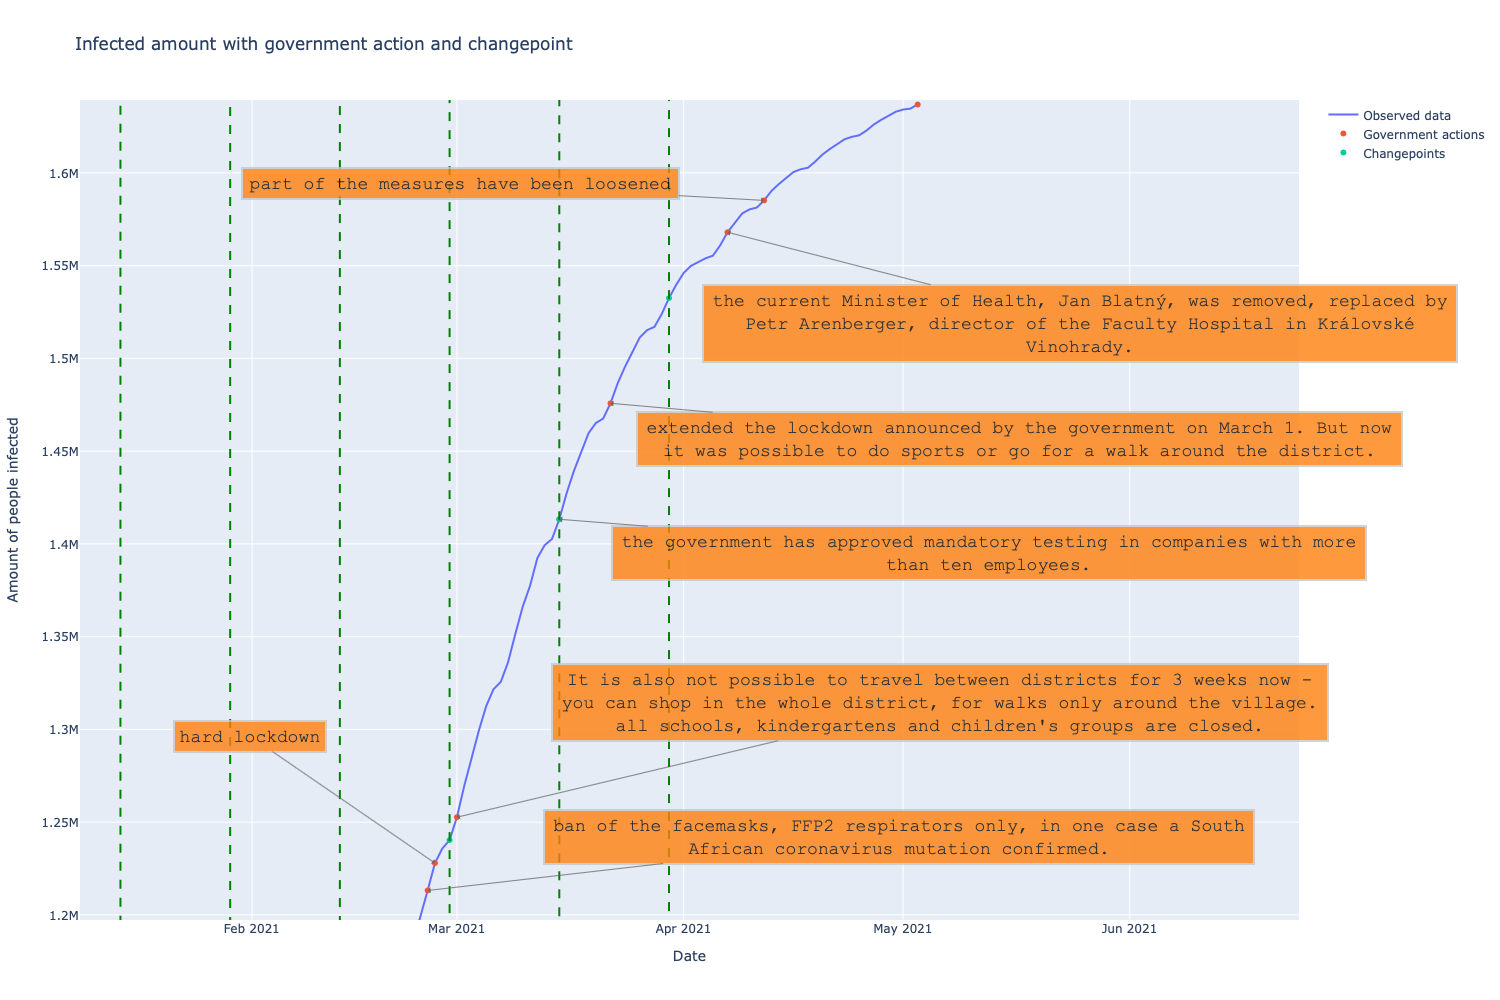
\includegraphics[width=1.0\textwidth, height=0.5\textwidth]{figures/chapter_04/changepoints_vs_government/infected_expo_to_lin_2nd}
\caption{Cumulative number of infected growth slowdown February-May 2021.}
\label{fig:corr_inf_e_l_2}
\end{figure}

We found out that before and during this time interval, the Czech government introduced the following important orders:
\begin{itemize}
    \item Wearing face masks was prohibited, FFP2 respirators only. (February 25, 2021).
    \item Hard lockdown was announced (February 26, 2021).
    \item Travel ban between districts for 3 weeks. All schools, kindergartens, and children's groups were closed. (March 1, 2021).
    \item Mandatory testing in companies with more than ten employees has been approved (March 15, 2021).
\end{itemize}

\subsubsection{Correlation: Number of infected explosive growth slowdown 3}

It is important to mention a growth slowing during the spring of 2020 (Figure \ref{fig:corr_inf_summer}). At this time, the Czech Republic has faced the beginning of the COVID-19 pandemic. According to Table \ref{tab:new_cases_mean_3}, mean number of people infected daily increased from 65.7 to 154.3 ($+234\%$) and then reduced to 66.5 ($-232\%$). 

\begin{table}[!htb]
\centering
\begin{tabular}{|l|l|l|}
\hline
Start date & End date & Mean number of active cases \\ \hline
2020-03-01 & 2020-04-06 & 65.7\\ \hline
2020-04-06 & 2020-04-21 & 154.3\\ \hline
2020-04-21 & 2020-05-06 & 66.5\\ \hline
\end{tabular}
\caption{Mean number of new cases daily between April 6, 2020 and May 6, 2020.}
\label{tab:new_cases_mean_3}
\end{table}

We discovered that before the beginning of the explosive increase of new cases, the government introduced the following important restrictions:
\begin{itemize}
    \item All primary, secondary, higher vocational, and university schools in the Czech Republic were closed until further notice (March 11, 2020).
    \item A state of emergency was declared in the Czech Republic for a period of 30 days (March 12, 2020).
    \item The operation of restaurants and shops was banned (March 14, 2020).
    \item State borders have been closed (with a few exceptions, March 16, 2020). 
\end{itemize}

\begin{figure}[!htb]
\centering
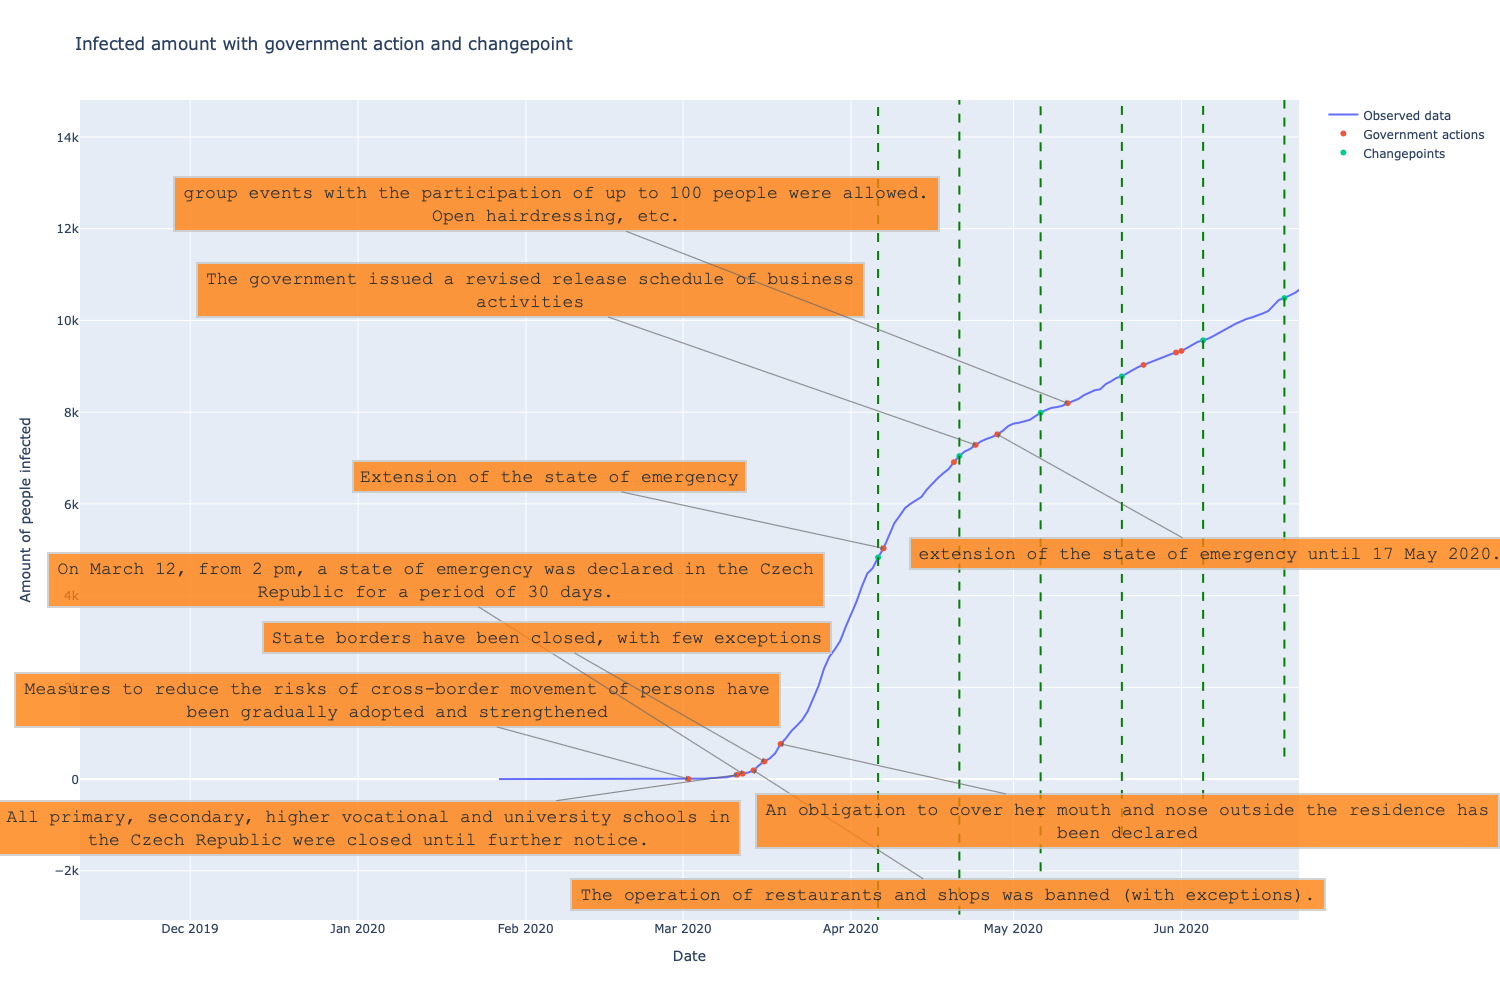
\includegraphics[width=1.0\textwidth, height=0.5\textwidth]{figures/chapter_04/changepoints_vs_government/infected_summer_stop.png}
\caption{Cumulative number of infected growth slowdown April-May 2020.}
\label{fig:corr_inf_summer}
\end{figure}

\subsection{Residual analysis}

Residual analysis is a fundamental step of the model diagnostics process. Thus, we decided to test the models introduced in Subsection \hyperlink{ss332}{3.3.2} and Subsection \hyperlink{ss333}{3.3.3}. 

\begin{figure}[!ht]
\centering
\subfloat[a][Cumulative number of new cases model: Residual analysis.]{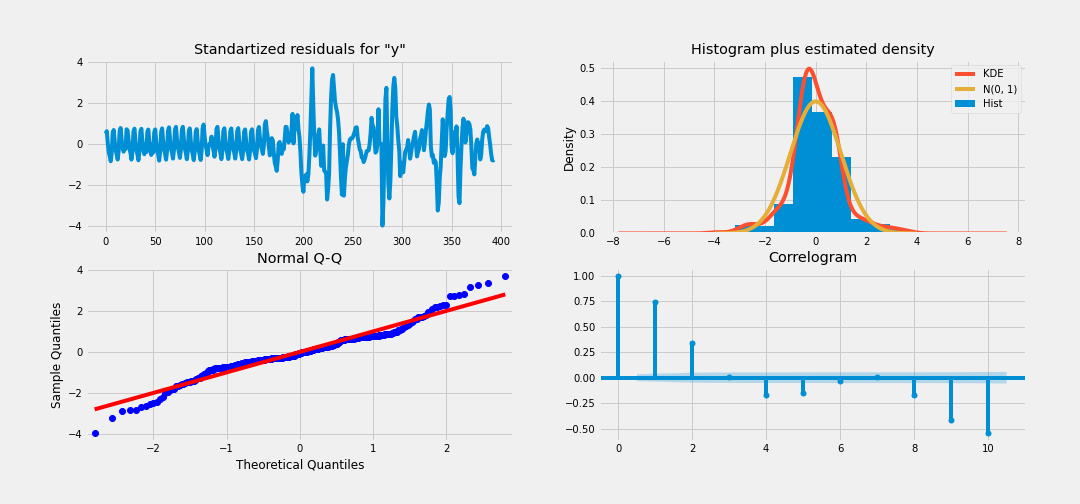
\includegraphics[width=1.0\textwidth, height=0.28\textwidth]{figures/chapter_04/prophet_resid_analysis/resid_prophet_infected.png}\label{fig:resid_infected}} \\
\subfloat[b][Cumulative number of people cured model: Residual analysis.]{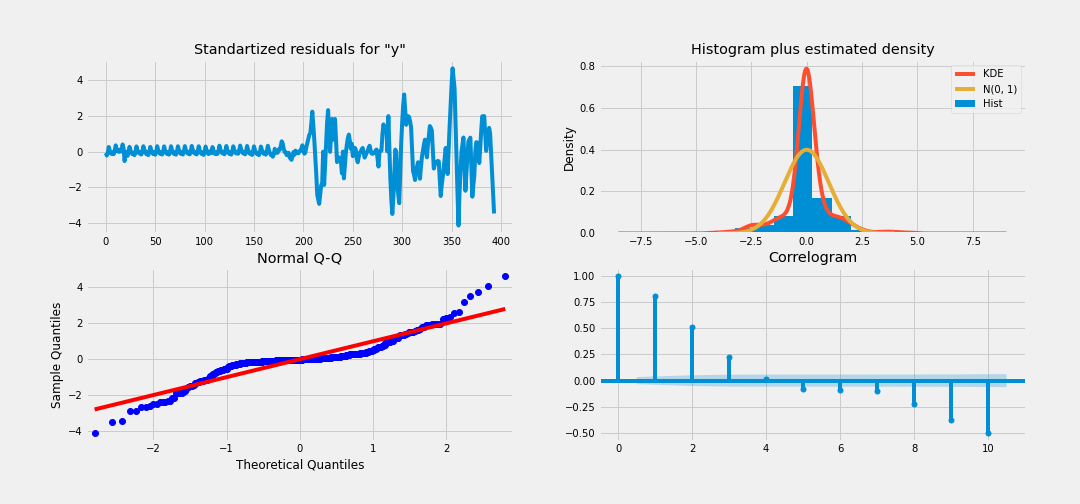
\includegraphics[width=1.0\textwidth, height=0.28\textwidth]{figures/chapter_04/prophet_resid_analysis/resid_prophet_cured.png}\label{fig:resid_cured}} \\
\subfloat[c][Cumulative number of people dead model: Residual analysis.]{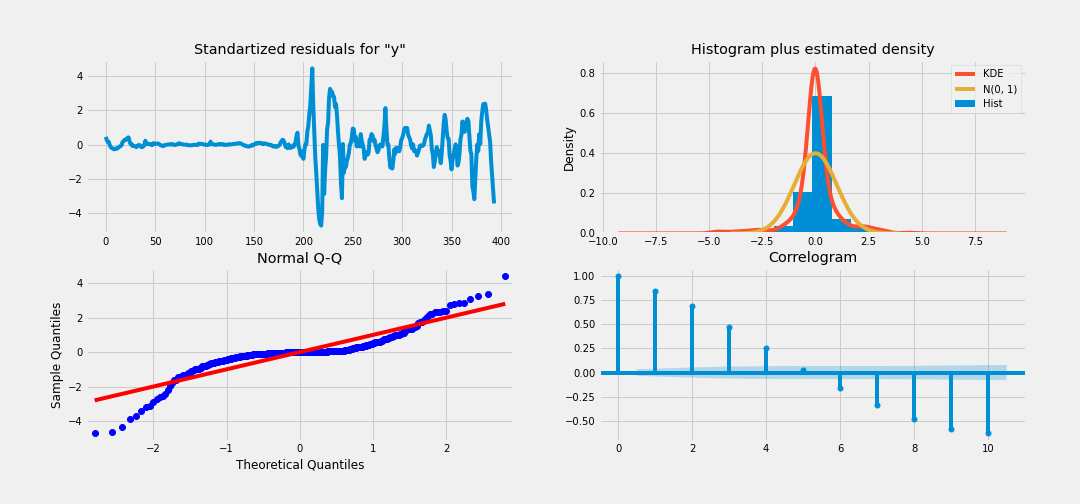
\includegraphics[width=1.0\textwidth, height=0.28\textwidth]{figures/chapter_04/prophet_resid_analysis/resid_prophet_dead.png}\label{fig:resid_dead}} \\
\subfloat[d][Number of active cases model: Residual analysis.]{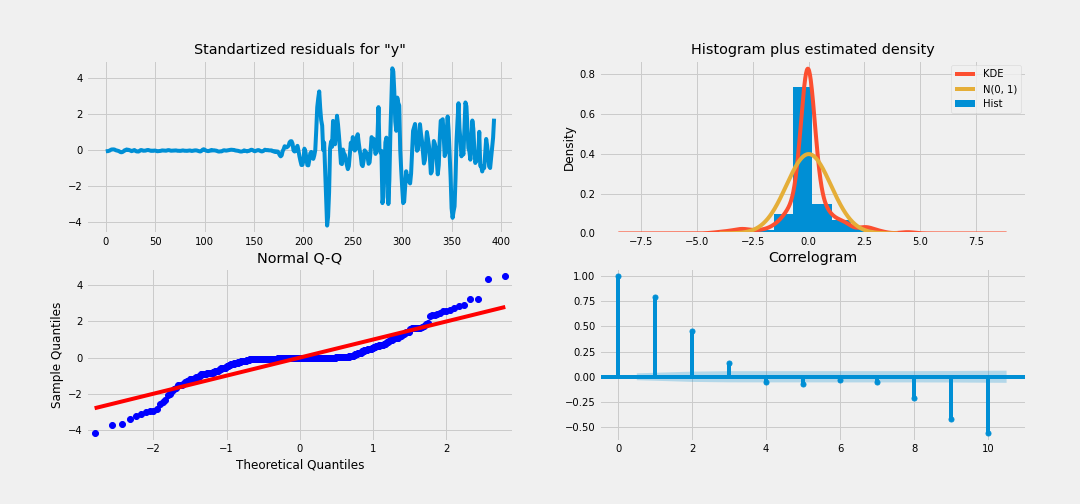
\includegraphics[width=1.0\textwidth, height=0.28\textwidth]{figures/chapter_04/prophet_resid_analysis/resid_prophet_active.png}\label{fig:resid_active}} \\
\caption{Residual analysis for the different Prophet models.}
\label{fig:resid_prophet}
\end{figure}

We consider models fitted to all historical data as more representative (in the context of the whole pandemic) than the models fitted to the data slices since the specific global changepoints and will perform their analysis first.

Analysis pipeline is specified, for example, in Hyndman et al. \cite{Hyndman2018} and contains the statistical testing of the probability that residuals are normally distributed (Jarque-Bera test), testing of the probability of correlation between residuals, and heteroscedasticity testing. Moreover, it implies different visualizations such as Q-Q plot, correlogram, and distribution histogram.

Figure \ref{fig:resid_prophet} demonstrates the different residual diagnostic plots. It is visible that all 4 models have some seasonal correlations between their residuals\footnote{\url{https://github.com/facebook/prophet/issues/1622} --- issue about residual problem in Prophet model. Almost all models have AR(1) relation in residuals. However, seasonal patters may indicate missing or not perfectly estimated seasonality.}. This may indicate that the models do not cover some seasonal relations in the data. Q-Q plots and histograms show that all 4 models do not have a normal distribution of the residuals. Additionally, Table \ref{tab:resid_testing_prophet_all}. contains the results of residual statistical testing\footnote{The Prophet model does not support residual heteroscedasticity testing.} that approve the information received from the visualizations above.

\begin{table}[!hbt]
\centering
\resizebox{\textwidth}{!}{%
\begin{tabular}{|l|l|l|l|}
\hline
Model        & Ljung-Box test                                                & Jarque-Bera test                                              & Heteroscedasticity test \\ \hline
\begin{tabular}[c]{@{}l@{}}Cumulative amount\\ of people infected\end{tabular} &
  \begin{tabular}[c]{@{}l@{}}p-value $\approx$ 0;\\ reject\end{tabular} &
  \begin{tabular}[c]{@{}l@{}}p-value $\approx$ 0;\\ reject\end{tabular} &
  - \\ \hline
\begin{tabular}[c]{@{}l@{}}Cumulative amount \\ of people cured\end{tabular} &
  \begin{tabular}[c]{@{}l@{}}p-value $\approx$ 0;\\ reject\end{tabular} &
  \begin{tabular}[c]{@{}l@{}}p-value $\approx$ 0;\\ reject\end{tabular} &
  - \\ \hline
\begin{tabular}[c]{@{}l@{}}Cumulative amount \\ of people dead\end{tabular} &
  \begin{tabular}[c]{@{}l@{}}p-value $\approx$ 0;\\ reject\end{tabular} &
  \begin{tabular}[c]{@{}l@{}}p-value $\approx$ 0;\\ reject\end{tabular} &
  - \\ \hline
Active cases & \begin{tabular}[c]{@{}l@{}}p-value $\approx$ 0;\\ reject\end{tabular} & \begin{tabular}[c]{@{}l@{}}p-value $\approx$ 0;\\ reject\end{tabular} & -                       \\ \hline
\end{tabular}%
}
\caption{Statistical residual testing of the Prophet models fitted to all historical data.}
\label{tab:resid_testing_prophet_all}
\end{table}

Now we can also perform the statistical residual testing of models fitted to the data slices. Table \ref{tab:resid_testing_prophet_slice} shows that the models fitted to the slices of the data with the information about the number of people cured and dead may have normally distributed residuals. However, we still can not reject that the residuals are correlated.

\begin{table}[!hbt]
\centering
\resizebox{\textwidth}{!}{%
\begin{tabular}{|l|l|l|l|}
\hline
Model        & Ljung-Box test                                                & Jarque-Bera test                                              & Heteroscedasticity test \\ \hline
\begin{tabular}[c]{@{}l@{}}Cumulative amount\\ of people infected\end{tabular} &
  \begin{tabular}[c]{@{}l@{}}p-value $\approx$ 0;\\ reject\end{tabular} &
  \begin{tabular}[c]{@{}l@{}}p-value $\approx$ 0;\\ reject\end{tabular} &
  - \\ \hline
\begin{tabular}[c]{@{}l@{}}Cumulative amount \\ of people cured\end{tabular} &
  \begin{tabular}[c]{@{}l@{}}p-value $\approx$ 0;\\ reject\end{tabular} &
  \begin{tabular}[c]{@{}l@{}}p-value = 0.98;\\ can not reject\end{tabular} &
  - \\ \hline
\begin{tabular}[c]{@{}l@{}}Cumulative amount \\ of people dead\end{tabular} &
  \begin{tabular}[c]{@{}l@{}}p-value $\approx$ 0.0001;\\ reject\end{tabular} &
  \begin{tabular}[c]{@{}l@{}}p-value = 0.21;\\ can not reject\end{tabular} &
  - \\ \hline
Active cases & \begin{tabular}[c]{@{}l@{}}p-value $\approx$ 0;\\ reject\end{tabular} & \begin{tabular}[c]{@{}l@{}}p-value $\approx$ 0;\\ reject\end{tabular} & -                       \\ \hline
\end{tabular}%
}
\caption{Statistical residual testing of the Prophet models fitted to the slices of historical data.}
\label{tab:resid_testing_prophet_slice}
\end{table}

\begin{figure}[!ht]
\centering
\subfloat[a][Cumulative number of new cases model: Residual analysis.]{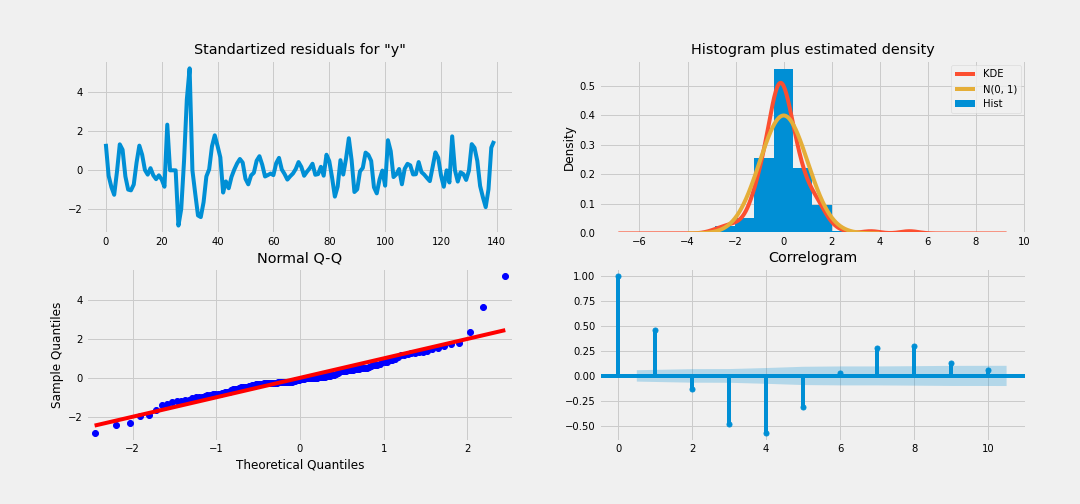
\includegraphics[width=1.0\textwidth, height=0.28\textwidth]{figures/chapter_04/prophet_resid_analysis/resid_prophet_infected_cp.png}\label{fig:resid_infected_slice}} \\
\subfloat[b][Cumulative number of people cured model: Residual analysis.]{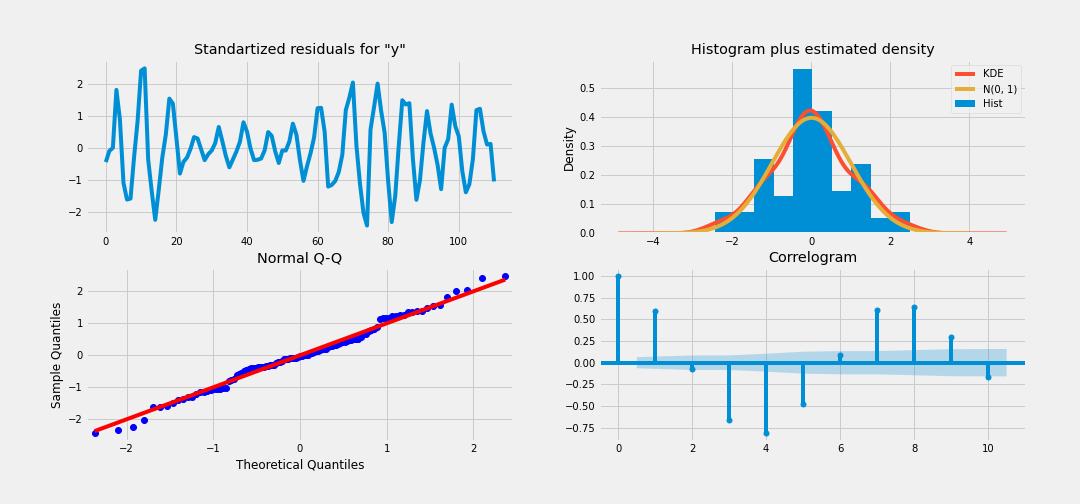
\includegraphics[width=1.0\textwidth, height=0.28\textwidth]{figures/chapter_04/prophet_resid_analysis/resid_prophet_cured_cp.png}\label{fig:resid_cured_slice}} \\
\subfloat[c][Cumulative number of people dead model: Residual analysis.]{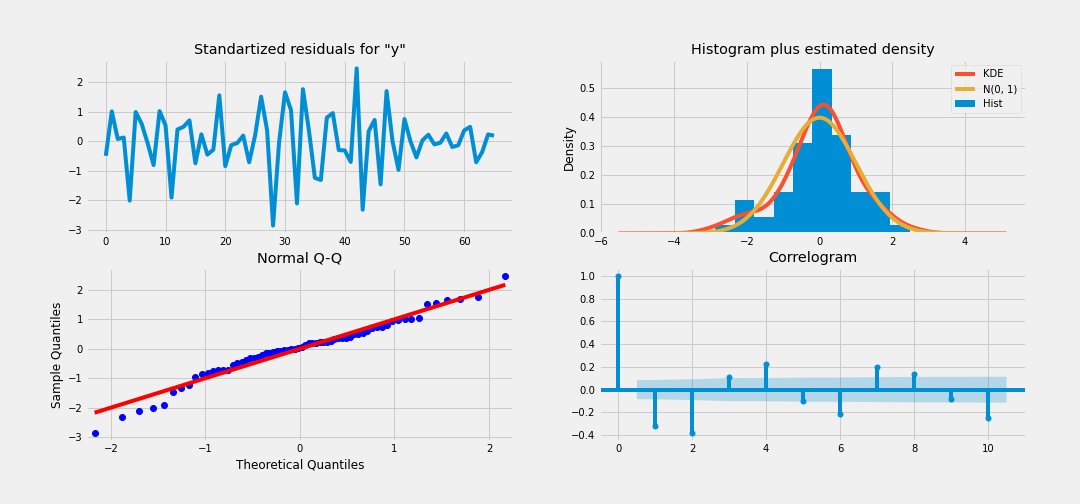
\includegraphics[width=1.0\textwidth, height=0.28\textwidth]{figures/chapter_04/prophet_resid_analysis/resid_prophet_dead_cp.png}\label{fig:resid_dead_slice}} \\
\subfloat[d][Number of active cases model: Residual analysis.]{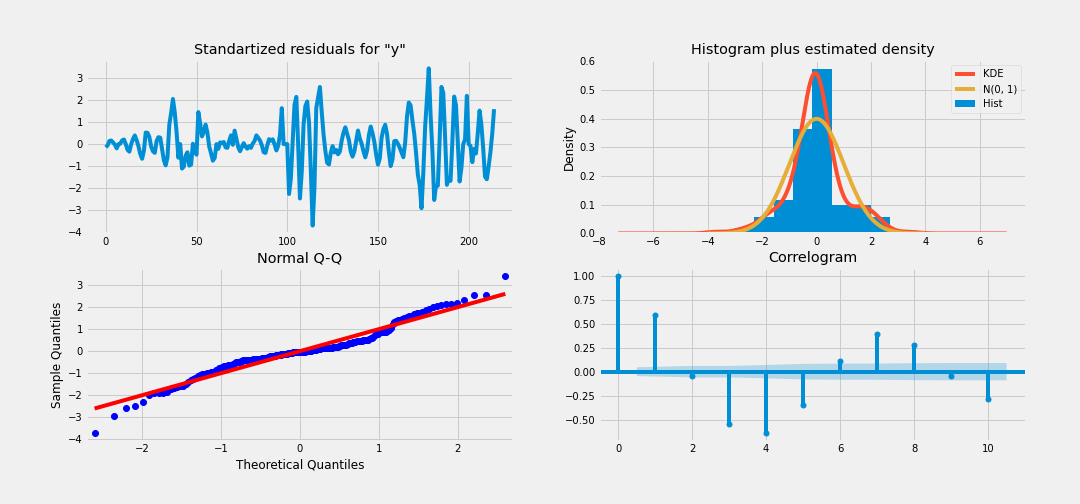
\includegraphics[width=1.0\textwidth, height=0.28\textwidth]{figures/chapter_04/prophet_resid_analysis/resid_prophet_active_cp.png}\label{fig:resid_active_slice}} \\
\caption{Residual analysis for the different Prophet models fitted to the slices of the historical data.}
\label{fig:resid_prophet_slices}
\end{figure}

In Figure \ref{fig:resid_prophet_slices} we can also see that in all models (except for the one that describes the number of deaths) some uncovered seasonal relations occur. The Q-Q plots and histogram indicates that all 4 models now have their residuals distributed more normally. This follows that fitting the model to the slice of the historical data reduces the number of uncovered processes that may influence this data.

% \subsection{Summary}

% // TODO //

\hypertarget{s3.4}{\section{SARIMA modeling}}

In this section, we perform modeling of the selected time series using SARIMA model implemented in Python library named \textit{statsmodels} \cite{seabold2010statsmodels}. It has all important functionalities for model fitting, forecast, and residual analysis.

\subsection{SARIMA model order estimation}

In Section \hypertarget{s3.2}{3.2} we have already estimated the order of the (S)ARIMA models which can be used for modeling the selected time series:
\begin{itemize}
    \item Cumulative number of people infected --- SARIMA(1, 1, 0)$\times$(1, 1, 0$)_7$.
    \item Cumulative number of people cured --- SARIMA(1, 1, 0)$\times$(1, 1, 0$)_7$.
    \item Cumulative number of people dead --- ARIMA(0, 2, 1).
    \item Number of active cases --- SARIMA(1, 1, 0)$\times$(1, 1, 0$)_7$.
\end{itemize}

\subsection{Forecasting using SARIMA}

Similar to the Facebook Prophet forecasts, for SARIMA modeling, we decided to use the 14 days forecast horizon. Moreover, we applied the logarithm transformation to the time series with information about active cases and dropped the first 55 days of measurements (to get rid of measurements with 0 value).

In Table \ref{tab:forecast_results_sarima_1} you can find information about MAPE on train data and on the forecast of new unseen 14 days of data. Models that describe the cumulative sum time series have a forecast MAPE between 0.68 \% and 0.80\%. In difference, the number of active case forecast MAPE is equal to 41.7\%.

\begin{table}[!ht]
\centering
\begin{tabular}{|l|l|l|}
\hline
Time series & Train MAPE & Forecast MAPE (\%)\\ \hline
\begin{tabular}[c]{@{}l@{}}Cumulative number \\ of people infected\end{tabular} &  1.440 &  0.800 \\ \hline
\begin{tabular}[c]{@{}l@{}}Cumulative number\\ of people cured\end{tabular}     &     1.580  &     0.680        \\ \hline
\begin{tabular}[c]{@{}l@{}}Cumulative number\\ of people dead\end{tabular}      &      1.320  &      0.720        \\ \hline
\begin{tabular}[c]{@{}l@{}}Number of active\\ cases\end{tabular}                &     4.710   &      41.760       \\ \hline
\end{tabular}%
\caption{Results of the original time series forecast using SARIMA models.}
\label{tab:forecast_results_sarima_1}
\end{table}

\begin{figure}[!ht]
\centering
\subfloat[a][Cumulative number of people infected time series forecast]{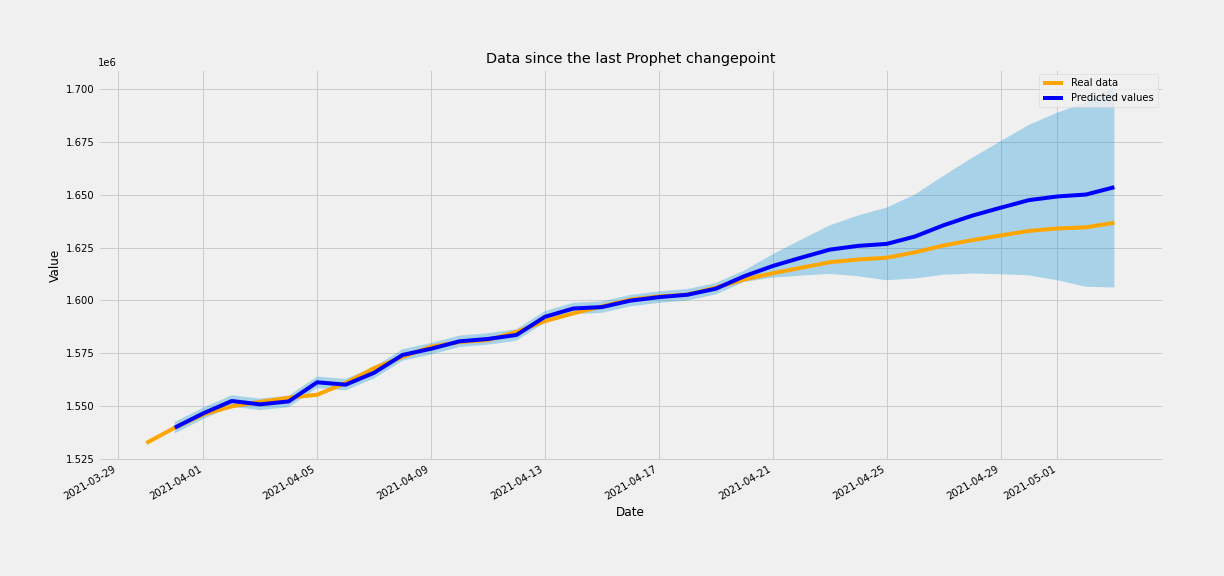
\includegraphics[width=1\textwidth, height=0.28\textwidth]{figures/chapter_04/sarima_forecast/sarima_forecast_infected.png}\label{fig:sarima_infected_forecast}} \\
\subfloat[b][Cumulative number of people cured time series forecast]{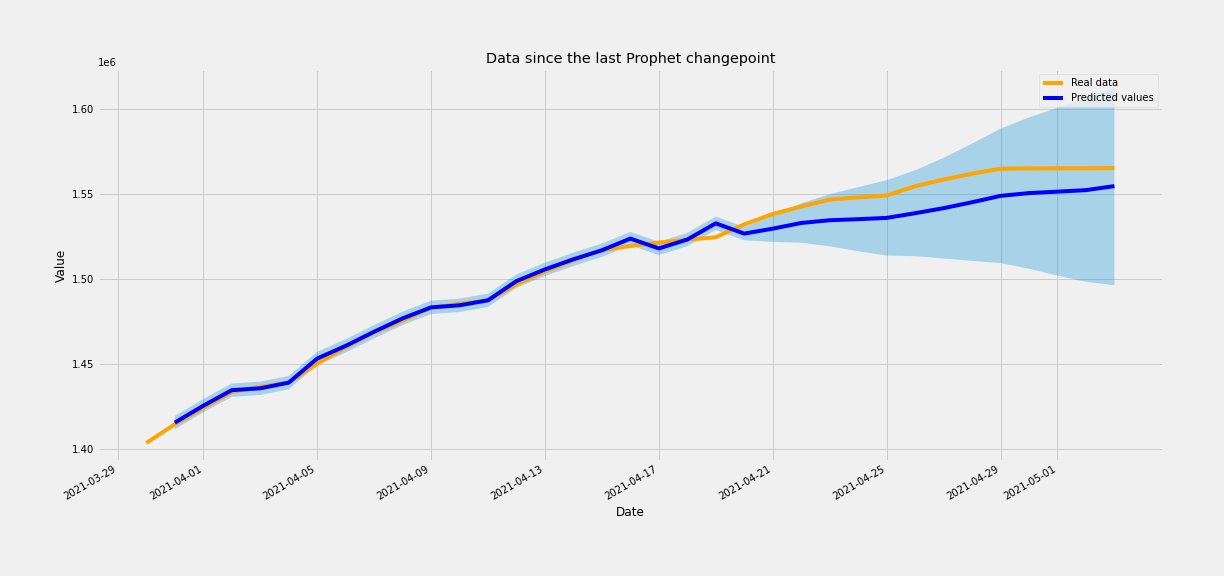
\includegraphics[width=1\textwidth, height=0.28\textwidth]{figures/chapter_04/sarima_forecast/sarima_forecast_cured.png}\label{fig:sarima_cured_forecast}} \\
\subfloat[c][Cumulative number of people dead time series forecast]{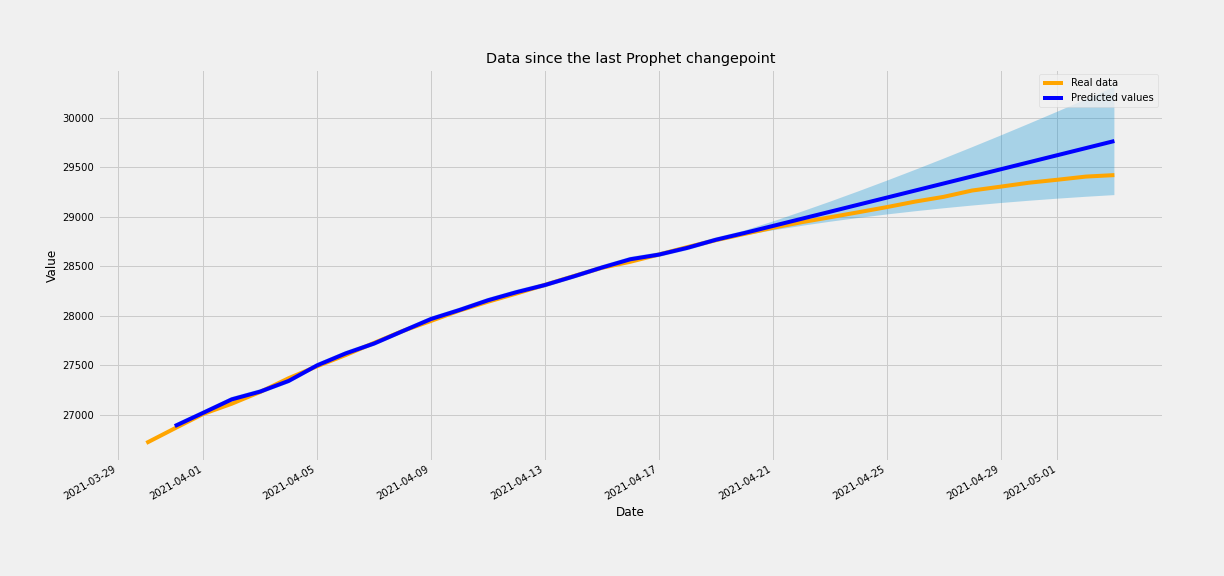
\includegraphics[width=1\textwidth, height=0.28\textwidth]{figures/chapter_04/sarima_forecast/sarima_forecast_dead.png}\label{fig:sarima_dead_forecast}} \\
\subfloat[d][Number of active cases time series forecast]{\includegraphics[width=1\textwidth, height=0.28\textwidth]{figures/chapter_04/sarima_forecast/sarima_forecast_active.png}\label{fig:sarima_active_forecast}} \\
\caption{The selected time series forecasts using SARIMA model.}
\label{fig:forecast_sarima}
\end{figure}

Figure \ref{fig:forecast_sarima} contains visualizations of the forecasts made. It covers the period since the last changepoint detected by Prophet (March 30, 2021). It is visible that the forecasts are relatively successful. However, the forecasted number of active cases differs distinctly from the real data. Confidence intervals become extremely wide after the first few days of each forecast.

\subsection{Changepoints usage influence on SARIMA model}

In the Prophet modeling section, we discovered that fitting the model to a slice of the historical data may improve the forecast results. This is possible because the selected COVID-19 time series change their development over time. In this subsection, we decided to study the influence of fitting the SARIMA model to the slices of data on the final forecast of the unseen data.

We fitted various models to the slices of the data since every changepoint detected in Section \hyperlink{ss333}{3.3.3}. Table \ref{tab:sarima_results_cp} contains information about the accuracy of the best forecasts obtained in this way for each time series.

\begin{table}[!ht]
\centering
\begin{tabular}{|l|l|l|l|}
\hline
Time series                                                                    & From date & Train MAPE (\%) & Test MAPE (\%) \\ \hline
\begin{tabular}[c]{@{}l@{}}Cumulative number\\ of people infected\end{tabular} &     2020-10-02      &     1.740       &       0.520    \\ \hline
\begin{tabular}[c]{@{}l@{}}Cumulative number \\ of people cured\end{tabular}   &     2020-12-30      &      9.590      &      3.780     \\ \hline
\begin{tabular}[c]{@{}l@{}}Cumulative number\\ of people dead\end{tabular}     &     2020-10-02     &     2.020       &     0.720     \\ \hline
\begin{tabular}[c]{@{}l@{}}Number of active \\ cases\end{tabular}              &     2021-03-15      &      3.620      &      8.950     \\ \hline
\end{tabular}
\caption{Best results of the time series forecast using SARIMA models fitted to the slices of data.}
\label{tab:sarima_results_cp}
\end{table}

According to these measurements, the prediction error of the number of new and active cases reduced from 0.8\% to 0.52\% and from 41.7\% to 8.95\%. However, the cumulative number of people dead forecast error did not change at all, and the cumulative number of people cured forecast error increased from 0.68\% to 3.78\%. 

Figure \ref{fig:forecast_sarima_cp} contains the corresponding forecast visualizations. On average, the confidence intervals became thinner (which indicates a reduction of the forecast uncertainty). Additionally, visualization (Figure \ref{fig:sarima_active_forecast_cp}) of the active case forecast demonstrates significant improvements. 

The results obtained during this experiment are mixed. Thus, we need to analyze the forecast residuals of all fitted models to conclude.


\begin{figure}[!ht]
\centering
\subfloat[a][Cumulative number of people infected time series forecast (data since October 2, 2020)]{\includegraphics[width=1\textwidth, height=0.25\textwidth]{figures/chapter_04/sarima_forecast/sarima_forecast_infected_cp.png}\label{fig:sarima_infected_forecast_cp}} \\
\subfloat[b][Cumulative number of people cured time series forecast (data since December 30, 2020)]{\includegraphics[width=1\textwidth, height=0.25\textwidth]{figures/chapter_04/sarima_forecast/sarima_forecast_cured_cp.png}\label{fig:sarima_cured_forecast_cp}} \\
\subfloat[c][Cumulative number of people dead time series forecast (data since October 2, 2020)]{\includegraphics[width=1\textwidth, height=0.25\textwidth]{figures/chapter_04/sarima_forecast/sarima_forecast_dead_cp.png}\label{fig:sarima_dead_forecast_cp}} \\
\subfloat[d][Number of active cases time series forecast (data since March 15, 2021)]{\includegraphics[width=1\textwidth, height=0.25\textwidth]{figures/chapter_04/sarima_forecast/sarima_forecast_active_cp.png}\label{fig:sarima_active_forecast_cp}} \\
\caption{The selected time series forecasts using SARIMA (since March 30, 2021) fitted to the slice of data since the specified changepoint}
\label{fig:forecast_sarima_cp}
\end{figure}

\subsection{Residual Analysis}

After fitting the SARIMA model, statsmodels allows us to perform residual analysis. Similar to the Prophet, we will use residual testing and visualization. 

\begin{figure}[!ht]
\centering
\subfloat[a][Cumulative number of new cases model: Residual analysis.]{\includegraphics[width=1.0\textwidth, height=0.28\textwidth]{figures/chapter_04/sarima_resid_analysis/residual_sarima_infected.png}\label{fig:resid_infected_s}} \\
\subfloat[b][Cumulative number of people cured model: Residual analysis.]{\includegraphics[width=1.0\textwidth, height=0.28\textwidth]{figures/chapter_04/sarima_resid_analysis/residual_sarima_cured.png}\label{fig:resid_cured_s}} \\
\subfloat[c][Cumulative number of people dead: Residual analysis.]{\includegraphics[width=1.0\textwidth, height=0.28\textwidth]{figures/chapter_04/sarima_resid_analysis/residual_sarima_dead.png}\label{fig:resid_dead_s}} \\
\subfloat[d][Cumulative number of active cases: Residual analysis.]{\includegraphics[width=1.0\textwidth, height=0.28\textwidth]{figures/chapter_04/sarima_resid_analysis/residual_sarima_active.png}\label{fig:resid_active_s}}\\
\caption{Residual analysis for the different SARIMA models.}
\label{fig:resid_sarima}
\end{figure}

First, we will analyze the models fitted to all historical data. 

According to Figure \ref{fig:resid_sarima}, number of new cases model has a residual correlation at lag 8, while the other 3 models may have uncorrelated residuals. However, according to the Ljung-Box test (Table \ref{tab:resid_testing_sarima}) we reject the hypothesis that the residuals are not correlated only for the model that describes the cumulative number of people dead time series. 

\begin{table}[!hbt]
\centering
\resizebox{\textwidth}{!}{%
\begin{tabular}{|l|l|l|l|}
\hline
Model        & Ljung-Box test                                                & Jarque-Bera test                                              & Heteroscedasticity test \\ \hline
\begin{tabular}[c]{@{}l@{}}Cumulative amount\\ of people infected\end{tabular} &
  \begin{tabular}[c]{@{}l@{}}p-value = 0.23;\\ can not reject\end{tabular} &
  \begin{tabular}[c]{@{}l@{}}p-value = 0.00;\\ reject\end{tabular} &
  \begin{tabular}[c]{@{}l@{}}p-value = 0.00;\\ reject \end{tabular} \\\hline
\begin{tabular}[c]{@{}l@{}}Cumulative amount \\ of people cured\end{tabular} &
  \begin{tabular}[c]{@{}l@{}}p-value = 0.37;\\ can not reject\end{tabular} &
  \begin{tabular}[c]{@{}l@{}}p-value = 0.00;\\ reject\end{tabular} &
  \begin{tabular}[c]{@{}l@{}}p-value = 0.00;\\ reject \end{tabular}\\ \hline
\begin{tabular}[c]{@{}l@{}}Cumulative amount \\ of people dead\end{tabular} &
  \begin{tabular}[c]{@{}l@{}}p-value = 0.00;\\ reject\end{tabular} &
  \begin{tabular}[c]{@{}l@{}}p-value = 0.00;\\ reject\end{tabular} &
  \begin{tabular}[c]{@{}l@{}}p-value = 0.00;\\ reject \end{tabular}\\ \hline
Active cases & \begin{tabular}[c]{@{}l@{}}p-value = 0.60;\\ can not reject\end{tabular} & \begin{tabular}[c]{@{}l@{}}p-value = 0.00;\\ reject\end{tabular} & \begin{tabular}[c]{@{}l@{}}p-value = 0.36;\\ can not reject      \end{tabular} \\ \hline
\end{tabular}%
}
\caption{Statistical residual testing of the SARIMA models fitted to all historical data.}
\label{tab:resid_testing_sarima}
\end{table}

Q-Q plots and histograms indicated that all 4 model residuals are not normally distributed. Jarque-Bera testing confirms it.  

The heteroscedasticity test indicates that the model that describes the number of active cases time series has residuals that do not change their structure over time (more relevant long-term forecasts). However, this result differs from the others because we applied a logarithm transformation to this time series (which reduces the heteroscedasticity in data). 

Now we can move to the residual analysis of the models fitted to the slices of the data since the specified changepoints.

\begin{table}[!hbt]
\centering
\resizebox{\textwidth}{!}{%
\begin{tabular}{|l|l|l|l|}
\hline
Model        & Ljung-Box test                                                & Jarque-Bera test                                              & Heteroscedasticity test \\ \hline
\begin{tabular}[c]{@{}l@{}}Cumulative amount\\ of people infected\end{tabular} &
  \begin{tabular}[c]{@{}l@{}}p-value = 0.00;\\ reject\end{tabular} &
  \begin{tabular}[c]{@{}l@{}}p-value = 0.00;\\ reject\end{tabular} &
  \begin{tabular}[c]{@{}l@{}}p-value = 0.00;\\ reject\end{tabular}\\ \hline
\begin{tabular}[c]{@{}l@{}}Cumulative amount \\ of people cured\end{tabular} &
  \begin{tabular}[c]{@{}l@{}}p-value = 0.00;\\ reject\end{tabular} &
  \begin{tabular}[c]{@{}l@{}}p-value = 0.00;\\ reject\end{tabular} &
  \begin{tabular}[c]{@{}l@{}}p-value = 0.26;\\ can not reject \end{tabular}\\ \hline
\begin{tabular}[c]{@{}l@{}}Cumulative amount \\ of people dead\end{tabular} &
  \begin{tabular}[c]{@{}l@{}}p-value = 0.23;\\ can not reject\end{tabular} &
  \begin{tabular}[c]{@{}l@{}}p-value = 0.73;\\ can not reject\end{tabular} &
  \begin{tabular}[c]{@{}l@{}}p-value = 0.64;\\ can not reject \end{tabular} \\ \hline
Active cases & \begin{tabular}[c]{@{}l@{}}p-value = 0.97;\\ can not reject\end{tabular} & \begin{tabular}[c]{@{}l@{}}p-value = 0.00;\\ reject\end{tabular} & \begin{tabular}[c]{@{}l@{}}p-value = 0.00; \\reject\end{tabular}\\ \hline
\end{tabular}%
}
\caption{Statistical residual testing of the SARIMA models fitted to slices of the historical data.}
\label{tab:resid_testing_sarima_slice}
\end{table}

According to Figure \ref{fig:resid_sarima_cp}, models that describe the cumulative number of people cured and infected now have correlated residuals. Ljung-Box test results (Table \ref{tab:resid_testing_sarima_slice}) confirm that. Their residuals also are not normally distributed.

\begin{figure}[!ht]
\centering
\subfloat[a][Cumulative number of new cases model: Residual analysis.]{\includegraphics[width=1.0\textwidth, height=0.28\textwidth]{figures/chapter_04/sarima_resid_analysis/residual_sarima_infected_cp.png}\label{fig:resid_infected_s_cp}} \\
\subfloat[b][Cumulative number of people cured model: Residual analysis.]{\includegraphics[width=1.0\textwidth, height=0.28\textwidth]{figures/chapter_04/sarima_resid_analysis/residual_sarima_cured_cp.png}\label{fig:resid_cured_s_cp}} \\
\subfloat[c][Cumulative number of people dead: Residual analysis.]{\includegraphics[width=1.0\textwidth, height=0.28\textwidth]{figures/chapter_04/sarima_resid_analysis/residual_sarima_dead_cp.png}\label{fig:resid_dead_s_cp}} \\
\subfloat[d][Number of active cases: Residual analysis.]{\includegraphics[width=1.0\textwidth, height=0.28\textwidth]{figures/chapter_04/sarima_resid_analysis/residual_sarima_active_cp.png}\label{fig:resid_active_s_cp}}\\
\caption{Residual analysis for the different SARIMA models fitted to the slices of data since specified changepoints.}
\label{fig:resid_sarima_cp}
\end{figure}

However, the number of people cured time series has heteroscedastic residuals (which may be helpful for long-term forecasts). 

The number of people dead model has noncorrelated, potentially normally distributed, heteroscedastic residuals and may be potentially used for long-term forecasts.

The number of active cases model also has noncorrelated residuals, but they are not heteroscedastic and not normally distributed.

\section{Results evaluation and discussion}

\subsection{Time series analysis results evaluation}

In Section \hyperlink{s3.2}{3.2} we performed the basic analysis of the selected time series. Using the theory studied during the theoretical research, we have found that:
\begin{itemize}
    \item It is possible to separate different processes and components that influence the evolution of the COVID-19 time series, such as global trend or seasonality (using the ACF and PACF).
    \item It is possible to estimate the order of the SARIMA model that can be used for modeling these time series, using methods that remove global trend and seasonality (differencing).
    \item The selected time series are changing their behavior over time. This fact requires the usage of models that can handle these changes.
\end{itemize}

This information is helpful for future analysis steps and reduces the number of problems that may occur during time series modeling using the Facebook Prophet or SARIMA model.

\subsection{Facebook Prophet modeling results evaluation}

In Section \hyperlink{s3.3}{3.3} we studied the possibility of modeling the COVID-19 time series using the Facebook Prophet model and obtained some interesting results. 

First, we discovered that it is possible to estimate proper hyperparameters using the inbuilt cross-validation technique. Models fitted using these parameters can achieve reasonable results.


Interestingly, the time series that contain the cumulative number of people infected, people cured, and people dead can be modeled without any data transformation. The number of active cases time series requires logarithm or Box-Cox transformation to reduce the measure of structural changes in the data. The forecasts made using the Prophet model fitted to all historical data are relatively accurate: the cumulative sum time series forecast error is within 0.8\% and 2.1\%. However, the number of active case predictions on average have 14\% error.  

Unexpectedly, the Facebook Prophet model residual analysis process has some potential problems (due to an incomplete model component). However, it is possible to detect some changes not covered by our models.

As expected, using the piecewise model allowed us to create a list of global trend changepoints. We can use them to improve the forecast accuracy by fitting the model to the slice of the data starting at these changepoints. Cumulative sum forecasts now have an error between 0.3\% and 0.4\%, active cases prediction error reduced to 7.9\%. This find indicates that the evolution of the COVID-19 processes changes over time. The measurements taken during the beginning may deter the modeling of further pandemic development.

The most striking observation to emerge from the Prophet analysis was the correlation detection between government restrictions and global slope changes. Specific examples can be found in Section \hyperlink{ss3.3.4}{3.3.4}.

All these results broaden our understanding of the COVID-19 pandemic modeling using the Facebook Prophet model.

\subsection{SARIMA modeling results evaluation}

Section \hyperlink{s3.4}{3.4} was aimed at the modeling of the COVID-19 processes using the SARIMA model. During this process, we used the information obtained from the time series analysis section to fit models of proper order.

Similar to the Prophet section, in the beginning, we used all historical data to fit the first bunch of models. The forecasts of the cumulative sums are used to have a high accuracy rate from the beginning (forecast error between 0.7-0.8\%). However, the prediction of the number of active cases was poor (forecast error equal to 41\%). Almost all these models (infected, cured, active) have wide confidence intervals (especially the model that describes the number of active cases). Nearly all models (except active cases) have non-heteroscedastic residuals, however, models that describe the number of active cases, people infected, and cured have their residuals noncorrelated. This find indicates that these models can be used only for short-term forecasts (few days).

We also evaluated the influence of fitting SARIMA models to the slices of the data. For this, we used the changepoints detected by the Prophet model. By doing this, we improved our prediction of active cases (error reduced from 41\% to 8.9\%), a cumulative number of people infected (0.8\% to 0.5\%). On the other side, the forecast accuracy of the number of people dead did not change at all, and the forecast of the number of people cured became less accurate (error increase from 0.7\% to 3.78\%).
It is important to say that the confidence intervals became much thinner. The residual analysis also demonstrates mixed results. 

In the case of the number of people dead time series, the residuals are noncorrelated, normally distributed, and heteroscedastic (this model may be helpful during long-term forecasts). However, the number of people cured and infected models now have a significant correlation between residuals. It may indicate the uncovered systematic processes that influence our model). 

These findings confirm those of the Prophet modeling section, such as fitting models to the slices of data makes the confidence interval thinner and, on average, decreases the forecast error. Moreover, it is now clear that sometimes we may see no improvement at all. It depends on the absence of major relations before the cutoff. 

Altogether, the results obtained with the SARIMA modeling are comparable to those obtained with the Prophet modeling. It is also possible to use the combination of these two models: to compare and supplement the results, or for changepoint detection with Prophet model and further usage in SARIMA modeling.

\setsecnumdepth{part}
\chapter{Conclusion}
At the beginning of 2020, the world was faced with a new disease called COVID-19. From the information-theoretic viewpoint, the pandemic is unique due to an abnormal number of available data sets. Many of them are in the form of time series.

The goal of this bachelor thesis was to perform statistical analyses of the selected time series related to the pandemic in the Czech Republic. For this, we have selected the time series with information about:
\begin{itemize}
    \item The cumulative number of people infected.
    \item The cumulative number of people cured.
    \item The cumulative number of people dead.
    \item The number of active cases.
\end{itemize}

\section{Theoretical research}

Before performing our modeling, we studied different literature aimed at theory related to the study of the time series. It allowed us to learn possible methods of time series analysis, decomposition, modeling, and further development prediction. 

According to the fact that the pandemic is a world problem, we have expected to find other publications and researches dedicated to the same problem. Reading and studying these materials assured us that it is possible to analyze the COVID-19 time series using statistical models and methods.

\section{Time series analysis}

After cleaning and preparing the selected data sets, it was necessary to perform basic time series analysis, such as decomposition of the trend, seasonal and cyclic components, and estimation of seasonal period duration. We also estimated the order of the autoregressive and moving average time series components for further SARIMA modeling. To do this, we used the information obtained by time series differencing and the analysis of the (partial) autocorrelation function. We have discovered that the selected time series change their behavior over time (nonstationarity). Moreover, all of them have global trend growth rate changes, nearly all of them have weekly seasonality. This find follows the usage of models that can handle these time series features.

\section{Model selection}

For this thesis, we decided to use the Facebook Prophet and Seasonal Autoregressive Moving Average (SARIMA) models. Both of them can handle seasonal nonstationary time series that change their evolution over time.

\section{Facebook Prophet modeling}

First, we decided to model the selected time series using the Facebook Prophet. We fitted the models to all the historical data. It allowed us to detect the trend changepoints (during the whole pandemic) for each time series individually. Interestingly, the cumulative sum time series can be forecasted with a high accuracy rate even without any special data preparation. However, the daily number of active cases required the data transformation (Box-Cox or logarithm) to reduce structural changes. Then we used the changepoints to fit new models to the data starting from these changepoints. After doing it, we improved the forecast accuracy for all selected time series. 

The Prophet model uses the piecewise trend concept to handle the global trend growth changes. We used this property to detect the correlations between the detected changepoints and various government restrictions that occurred during the pandemic. The most striking observation to emerge from the correlation analysis was the correlation between the reduction of the daily mean number of new cases and the government restrictions aimed at wearing face masks (respirators), social distancing, and (partial) lockdown.

\section{SARIMA modeling}

The next step was SARIMA modeling. To select the proper order of autoregressive and moving average components, we used the information obtained during the time series analysis. Similarly to the Prophet modeling, the first bunch of models was fitted to all available historical data. In this case, the prediction accuracy was comparable to that obtained using the Prophet model, however, the number of active cases prediction was poor (MAPE = 41\%), and the confidence intervals were broad (except the number of people dead forecast). 

As the next step of the analysis, we explored the potential synergy between the SARIMA model and trend changepoints obtained using the Prophet model. 

The outcome was not that unambiguous like in the case of the Prophet model: some forecasts became less accurate, however, the confidence intervals became thinner. It follows that fitting the model to the slice of the historical data since the specified trend changepoint may improve the forecast only if the earlier data do not contain essential information about the processes that influence time series development.

\section{Summary}

In this thesis, we discovered that it is possible to perform the COVID-19 analysis using statistical analysis and modeling. We found out that the Facebook Prophet and SARIMA models allow receiving significant results and can be used in combination or in isolation. However, because of the unstable evolution of the pandemic processes, only the first few days of the forecast can be used in practice.

\section{Future work}

This study provides the backbone for several possible extensions. First, using the judgmental forecast methods (described, for example, in Hyndman et al. \cite{Hyndman2018}) in association with an epidemiology expert may improve prediction accuracy and result interpretation. Second, it is possible to extend a list of the selected time series by including vaccination, reproductive number, distribution of new cases severity, and so on. It will expand the search range for possible anomalies and interesting phenomena within the time series. Moreover, it is reasonable to test various data preparation and transformation techniques that are not discussed in this thesis.  

\bibliographystyle{bibtex/iso690}
\bibliography{bibtex/bib-database}

\setsecnumdepth{all}
\appendix

\chapter{Acronyms}
% \printglossaries
\begin{description}
    \item[ACF] Autocorrelation function
    \item[AIC] Akaike information criterion
	\item[AR] Autoregressive 
	\item[ARMA] Autoregressive Moving Average
	\item[ARIMA] Autoregressive Integrated Moving Average
	\item[BIC] Bayesian information criterion
	\item[KPSS] Kwiatkowski–Phillips–Schmidt–Shin
	\item[MA] Moving average
	\item[MAPE] Mean Absolute Percentage Error
	\item[MLE] Maximum Likelihood Estimation
	\item[PACF] Partial autocorrelation function
	\item[Q-Q] Quantile-Quantile plot
	\item[SARIMA] Seasonal Autoregressive Integrated Moving Average
	\item[STL] Seasonal-trend decomposition
\end{description}


\chapter{Contents of enclosed CD}

%change appropriately

\begin{figure}
	\dirtree{%
		.1 readme.txt\DTcomment{the file with CD contents description}.
		.1 src\DTcomment{the directory of source codes}.
		.2 data\DTcomment{used data sets}.
		.2 functions\DTcomment{used external functions}.
		.2 notebooks\DTcomment{Jupyter notebooks with analysis}.
		.2 thesis\DTcomment{the directory of \LaTeX{} source codes of the thesis}.
		.1 texts\DTcomment{the thesis text directory}.
		.2 thesis\_Oleh\_Kuznetsov.pdf\DTcomment{the thesis text in PDF format}.
	}
\end{figure}

\end{document}
